%% LyX 2.2.2 created this file.  For more info, see http://www.lyx.org/.
%% Do not edit unless you really know what you are doing.
\documentclass[english,magyar]{article}
\usepackage[T1]{fontenc}
\usepackage[latin9,latin2]{inputenc}
\usepackage{geometry}
\geometry{verbose,tmargin=2cm,bmargin=2cm,lmargin=1cm,rmargin=1cm,headheight=1cm,headsep=1cm,footskip=1cm}
\usepackage{color}
\definecolor{shadecolor}{rgb}{0.335938, 0.667969, 1}
\usepackage{babel}
\usepackage{float}
\usepackage{wrapfig}
\usepackage{fancybox}
\usepackage{calc}
\usepackage{framed}
\usepackage{amsmath}
\usepackage{amsthm}
\usepackage{amssymb}
\usepackage{graphicx}
\PassOptionsToPackage{normalem}{ulem}
\usepackage{ulem}
\usepackage[unicode=true]
 {hyperref}

\makeatletter

%%%%%%%%%%%%%%%%%%%%%%%%%%%%%% LyX specific LaTeX commands.
%% Because html converters don't know tabularnewline
\providecommand{\tabularnewline}{\\}

%%%%%%%%%%%%%%%%%%%%%%%%%%%%%% Textclass specific LaTeX commands.
\theoremstyle{plain}
\newtheorem{thm}{\protect\theoremname}
\theoremstyle{definition}
\newtheorem{xca}[thm]{\protect\exercisename}

\@ifundefined{showcaptionsetup}{}{%
 \PassOptionsToPackage{caption=false}{subfig}}
\usepackage{subfig}
\makeatother

\addto\captionsenglish{\renewcommand{\exercisename}{Exercise}}
\addto\captionsenglish{\renewcommand{\theoremname}{Theorem}}
\addto\captionsmagyar{\renewcommand{\exercisename}{Gyakorlat}}
\addto\captionsmagyar{\renewcommand{\theoremname}{T�tel}}
\providecommand{\exercisename}{Gyakorlat}
\providecommand{\theoremname}{T�tel}

\begin{document}

\title{Statisztikus Fizika Gyakorlat}

\maketitle
\medskip{}
\medskip{}

\begin{center}
``Ludwig Boltzmann, who spent much of his life studying statistical
mechanics, died in 1906, by his own hand. 
\par\end{center}

\begin{center}
Paul Ehrenfest, carrying on the work, died similarly in 1933. 
\par\end{center}

\begin{center}
Now it is our turn to study statistical mechanics.'' 
\par\end{center}

\medskip{}
\medskip{}
\medskip{}

\begin{center}
DAVID L. GOODSTEIN 
\par\end{center}

\begin{center}
in 
\par\end{center}

\begin{center}
STATES OF MATTER
\par\end{center}

\inputencoding{latin2}%

\part{N�h�ny hasznos matematikai formula}

\section{\protect\href{https://en.wikipedia.org/wiki/Gaussian_integral}{Gauss-integr�l}}

Vezess�k le a k�vetkez� integr�lt:

\begin{shaded}%
\begin{equation}
I=\int_{-\infty}^{\infty}\mathrm{e}^{-x^{2}}\mathrm{d}x=\sqrt{\pi}.\label{eq:gauss-0}
\end{equation}
\end{shaded}C�lszer� a kifejez�s n�gyzet�t vizsg�lni!

\begin{equation}
I^{2}=\int_{-\infty}^{\infty}\int_{-\infty}^{\infty}\mathrm{e}^{-x^{2}-y^{2}}\mathrm{d}x\mathrm{d}y.\label{eq:gauss-levezet-1}
\end{equation}
Az integr�lt �rjuk �t pol�rkoordin�t�kba!

\begin{eqnarray}
x & = & r\cos\varphi,\label{eq:gauss-polar}\\
y & = & r\sin\varphi,\nonumber \\
\mathrm{d}x\mathrm{d}y & = & r\mathrm{d}\varphi\mathrm{d}r.\nonumber 
\end{eqnarray}
A keresett integr�l a k�vetkez� alakot �lti:

\begin{equation}
I^{2}=\int_{0}^{\infty}\int_{0}^{2\pi}\mathrm{e}^{-r^{2}}r\mathrm{d}\varphi\mathrm{d}r=2\pi\int_{0}^{\infty}\mathrm{e}^{-r^{2}}r\mathrm{d}r.\label{eq:gauss-levezet-2}
\end{equation}

\textcolor{blue}{\emph{Megjegyz�s:}}\textcolor{blue}{{} Vegy�k �szre,
hogy m�g a pol�rkoordin�t�kn�l $0$-t�l $\infty$-ig integr�ltunk,
az eredeti integr�lunk $-\infty$-t�l $\infty$-ig megy. Itt nem k�vett�nk
el semmilyen matematikai hib�t ugyanis ezt a sz�gf�gg�ssel figyelembe
vett�k a pol�rkoordin�t�k seg�ts�g�vel.}\\
V�gezz�nk el m�g egy v�ltoz� cser�t!

\begin{eqnarray}
u & = & r^{2},\label{eq:gauss-rtou}\\
\frac{\mathrm{d}u}{\mathrm{d}r} & = & 2r\rightarrow\mathrm{d}r=\frac{\mathrm{d}u}{2r}.\nonumber 
\end{eqnarray}
�gy m�r elemi integr�ci�s szab�lyokkal ki�rt�kelhet� �sszef�gg�sre
jutunk:

\begin{equation}
I^{2}=2\pi\int_{0}^{\infty}\frac{\mathrm{e}^{-u}}{2}\mathrm{d}u=\pi\left[-\mathrm{e}^{-u}\right]_{0}^{\infty}=\pi.\label{eq:gauss-levezet-3}
\end{equation}
A keresett integr�l teh�t:

\begin{equation}
\int_{-\infty}^{\infty}\mathrm{e}^{-x^{2}}\mathrm{d}x=\sqrt{\pi}.\label{eq:gauss-eredmeny}
\end{equation}
Egy egyszer� v�ltoz� cser�vel l�ssuk be a Gauss-integr�l egyszer�
�ltal�nos�t�s�t:

\begin{shaded}%
\begin{equation}
\int_{-\infty}^{\infty}\mathrm{e}^{-ax^{2}}\mathrm{d}x=\sqrt{\frac{\pi}{a}}.\label{eq:gauss-scaled}
\end{equation}
\end{shaded}

\begin{align}
ax^{2} & =t^{2},\\
\frac{\mbox{d}t}{\mbox{d}x} & =\sqrt{a}\rightarrow\mbox{d}t=\sqrt{a}\mbox{d}x.
\end{align}
Kapjuk teh�t hogy
\begin{equation}
\int_{-\infty}^{\infty}\mathrm{e}^{-ax^{2}}\mathrm{d}x=\int_{-\infty}^{\infty}\mathrm{e}^{-t^{2}}\frac{\mbox{d}t}{\sqrt{a}}=\sqrt{\frac{\pi}{a}}.
\end{equation}

\shadowbox{\begin{minipage}[t]{0.9\columnwidth}%
\begin{xca}
L�ssuk be hogy ha $a>0$ val�s sz�m akkor:
\end{xca}
\begin{equation}
\int_{-\infty}^{\infty}\mathrm{e}^{-ax^{2}+bx+c}\mathrm{d}x=\sqrt{\frac{\pi}{a}}e^{\frac{b^{2}}{4a}+c}\label{eq:gauss-alltalanos}
\end{equation}

�tmutat�s:
\begin{itemize}
\item Alak�tsuk teljes n�gyzett� a kitev�ben szerepl� polinomot! 
\item A Gauss-integr�l invari�ns az integrandus ``eltol�s�ra''! 
\item A n�gyzetes tag egy�tthat�j�t�l egy alkalmas v�ltoz� cser�vel szabadulhatunk
meg. 
\end{itemize}
%
\end{minipage}}

\section{A \protect\href{https://hu.wikipedia.org/wiki/Gamma-f\%C3\%BCggv\%C3\%A9ny}{Gamma-f�ggv�ny}
n�h�ny tulajdons�ga}

\begin{figure}[H]
\begin{centering}
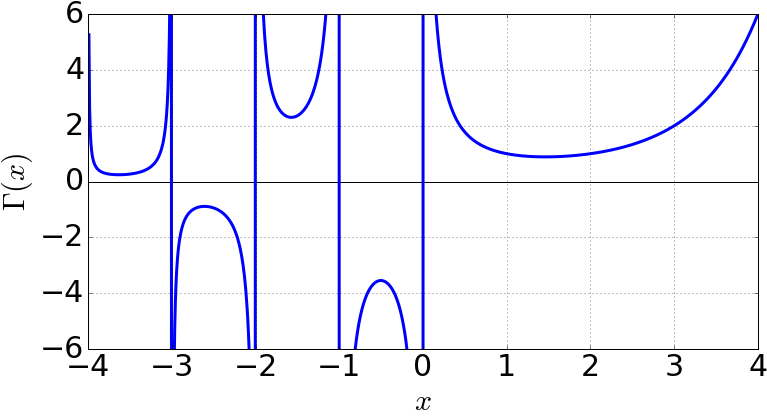
\includegraphics[width=0.5\textwidth]{Fig/Gamma}
\par\end{centering}
\caption{A Gamma f�ggv�ny\label{fig:A-Gamma-fuggveny}}

\end{figure}

\begin{shaded}%
\textbf{A Gamma-f�ggv�ny:}

\begin{equation}
\Gamma(x)=\int_{0}^{\infty}\mathrm{e}^{-t}t^{x-1}\mathrm{d}t,\quad\mathrm{Re}(x)>0,\label{eq:gamma-def}
\end{equation}
\end{shaded}

A fenti defin�ci� seg�ts�g�vel l�ssuk be hogy

\begin{shaded}%
\begin{equation}
\Gamma(x+1)=x\Gamma(x).\label{eq:gamma-plusone}
\end{equation}
\end{shaded}

\begin{eqnarray}
\Gamma(x+1) & = & \int_{0}^{\infty}\underbrace{\mbox{e}^{-t}}_{v'}\underbrace{t^{x}}_{u}\mbox{d}t\label{eq:gamma-levezet-1}\\
 & = & \underbrace{[t^{x}(-\mbox{e}^{-t})]_{0}^{\infty}}_{0}-\int_{0}^{\infty}\underbrace{-\mbox{e}^{-t}}_{v}\underbrace{xt^{x-1}}_{u'}\mbox{d}t\\
 & = & x\int_{0}^{\infty}\mbox{e}^{-t}t^{x-1}\mbox{d}t\\
 & = & x\Gamma(x)
\end{eqnarray}
ahol kihaszn�ltuk a parci�lis integr�l�s szab�ly�t

\begin{equation}
\int u(t)v'(t)\mbox{d}t=u(t)v(t)-\int u'(t)v(t)\mbox{d}t
\end{equation}
�s az al�bbi k�t ismert �sszef�gg�st

\begin{eqnarray}
\int\mbox{e}^{\alpha t}\mbox{d}t & = & \frac{\mbox{e}^{\alpha t}}{\alpha},\\
\partial_{t}t^{\alpha} & = & \alpha t^{\alpha-1}.
\end{eqnarray}
L�ssuk be a k�vetkez� k�t �sszef�gg�st is!

\begin{shaded}%
\begin{eqnarray}
\Gamma(1) & = & 1\label{eq:gamma-one}\\
\Gamma\left(\frac{1}{2}\right) & = & \sqrt{\pi}\label{eq:gamma-half}
\end{eqnarray}
\end{shaded}

\begin{eqnarray}
\Gamma(1) & = & \int_{0}^{\infty}\mbox{e}^{-t}t^{1-1}\mbox{d}t\\
 & = & \int_{0}^{\infty}\mbox{e}^{-t}\mbox{d}t\\
 & = & [-\mbox{e}^{-t}]_{0}^{\infty}=1
\end{eqnarray}
Felhaszn�lva a (\ref{eq:gamma-plusone}) �s (\ref{eq:gamma-one})
�sszef�gg�seket a $\Gamma(x)$ f�ggv�nyt tetsz�leges pozit�v eg�sz
sz�mokra meghat�rozhatjuk:

\begin{eqnarray}
\Gamma(2) & = & 1\Gamma(1)=1\\
\Gamma(3) & = & 2\Gamma(2)=2\cdot1\\
\Gamma(4) & = & 3\Gamma(3)=3\cdot2\cdot1
\end{eqnarray}

\begin{shaded}%
\begin{equation}
\Gamma(n)=(n-1)!\quad n\in\mathbb{N}\label{eq:gamma-factorial}
\end{equation}
\end{shaded}

\begin{eqnarray}
\Gamma(1/2) & = & \int_{0}^{\infty}\mbox{e}^{-t}t^{1/2-1}\mbox{d}t\\
 & = & \int_{0}^{\infty}\frac{\mbox{e}^{-t}}{t^{1/2}}\mbox{d}t
\end{eqnarray}
Hajtsuk v�gre a k�vetkez� v�ltoz� cser�t:

\begin{eqnarray}
u & = & t^{1/2},\\
\frac{\mbox{d}u}{\mbox{d}t} & = & \frac{1}{2}\frac{1}{t^{1/2}}.
\end{eqnarray}
�gy kapjuk hogy

\begin{eqnarray}
\int_{0}^{\infty}\frac{\mbox{e}^{-t}}{t^{1/2}}\mbox{d}t & = & \int_{0}^{\infty}\mbox{e}^{-u^{2}}2\mbox{d}u,\\
 & = & \int_{-\infty}^{\infty}\mbox{e}^{-u^{2}}\mbox{d}u=\sqrt{\pi}.
\end{eqnarray}
\begin{figure}[H]
\begin{centering}
\subfloat[A Stirling-formula levezet�se sor�n alkalmazott k�zel�t�s \label{fig:Stirling formula-integrand}]{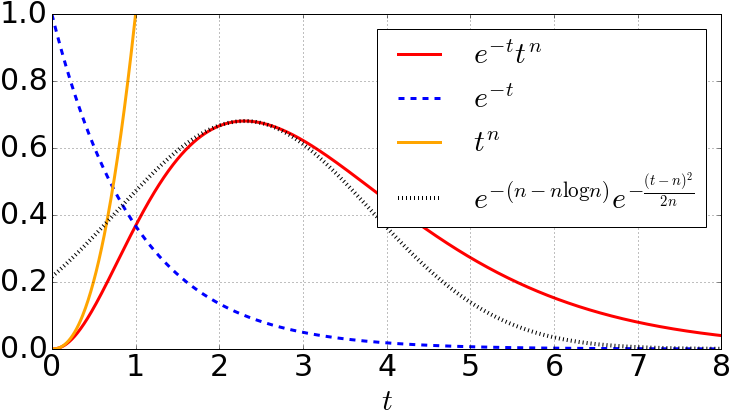
\includegraphics[width=0.4\textwidth]{Fig/Stirling}}
$\quad\quad\quad\quad$\subfloat[A Stirling-formula �s a $\Gamma$-f�ggv�ny ]{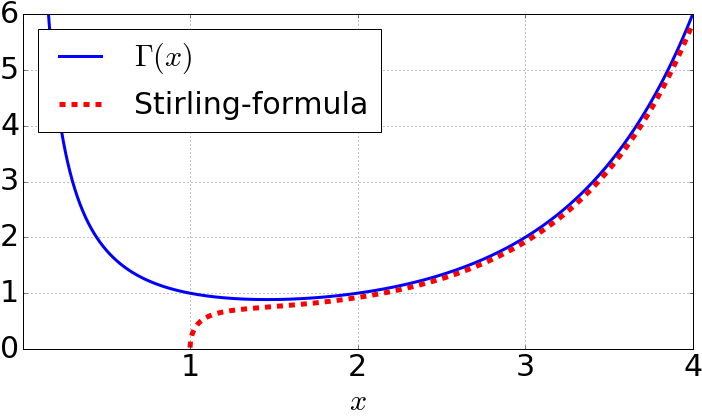
\includegraphics[width=0.4\textwidth]{Fig/Stirling-approx}

}
\par\end{centering}
\caption{Stirling k�zel�t�s}
\end{figure}

Termodinamikai hat�resetek vizsg�lata sor�n sokszor fogunk tal�lkozni
olyan esetekkel amikor a $\Gamma(n)$ f�ggv�nyt a $n\gg1$ �rt�kekre
kell ki�rt�keln�nk. 

L�ssuk be a k�vetkez� hasznos k�zel�t� formul�t:

\begin{shaded}%
\textbf{\href{https://hu.wikipedia.org/wiki/Stirling-formula}{Stirling-formula:}}
\begin{equation}
n!=n^{n}\mbox{e}^{-n}\sqrt{2\pi n}\left(1+\mathcal{O}\left(\frac{1}{n}\right)\right)\label{eq:stirling-formula}
\end{equation}
\end{shaded}
\begin{align}
n! & =\Gamma(n+1)=\int_{0}^{\infty}\mbox{e}^{-t}t^{n}\mbox{d}t\label{eq:stirling-init}\\
 & =\int_{0}^{\infty}\mbox{e}^{-t+n\ln t}\mbox{d}t\nonumber \\
 & =\int_{0}^{\infty}\mbox{e}^{-f_{n}(t)}\mbox{d}t,\nonumber \\
f_{n}(t) & =t-n\ln t.
\end{align}
Fejts�k sorba az $f_{n}(t)$ f�ggv�nyt a minimuma k�r�l!
\begin{equation}
\partial_{t}f_{n}(t)=1-\frac{n}{t},
\end{equation}
\begin{equation}
\partial_{t}f_{n}(t_{0})=0\rightarrow t_{0}=n.
\end{equation}
Elegend� elv�gezni a sorfejt�st m�sod rendig. Azaz a k�vetkez� k�zel�t�ssel
�l�nk:
\begin{equation}
f_{n}(t)\approx f_{n}(t_{0})+\partial_{t}f_{n}(t_{0})\left(t-t_{0}\right)+\frac{1}{2}\partial_{t}^{2}f_{n}(t_{0})\left(t-t_{0}\right)^{2},
\end{equation}
\begin{equation}
\partial_{t}^{2}f_{n}(t)=\frac{n}{t^{2}}\rightarrow\partial_{t}^{2}f_{n}(t_{0})=\frac{n}{n^{2}}=\frac{1}{n},
\end{equation}
\begin{equation}
f_{n}(t)\approx n-n\ln n+\underbrace{\partial_{t}f_{n}(t_{0})\left(t-t_{0}\right)}_{\text{by def}=0}+\frac{1}{2}\left(\frac{1}{n}\right)\left(t-n\right)^{2}.
\end{equation}
Vissza�rva ezt a \eqref{eq:stirling-init} kifejez�sbe:
\begin{align}
n! & =\int_{0}^{\infty}\mbox{e}^{-t}t^{n}\mbox{d}t\\
 & =\int_{0}^{\infty}\mbox{e}^{-f_{n}(t)}\mbox{d}t\nonumber \\
 & \approx\mbox{e}^{-\left(n-n\ln n\right)}\int_{0}^{\infty}\mbox{e}^{-\frac{\left(t-n\right)^{2}}{2n}}\mbox{d}t.\nonumber 
\end{align}
A kifejez�sben szerepl� integr�l als� hat�r�t kiterjeszthetj�k $-\infty$-ig
hiszen feltett�k hogy $n\gg1$:
\begin{align}
n! & \approx\mbox{e}^{-\left(n-n\ln n\right)}\int_{-\infty}^{\infty}\mbox{e}^{-\frac{\left(t-n\right)^{2}}{2n}}\mbox{d}t\\
 & =\mbox{e}^{-\left(n-n\ln n\right)}\sqrt{2\pi n}.\nonumber 
\end{align}
Ahol felhaszn�ltuk a Gauss-integr�lra vonatkoz� \eqref{eq:gauss-scaled}
azonoss�got. A kapott eredm�ny pedig nem m�s mint maga a \eqref{eq:stirling-formula}
Stirling-formula. Sokszor fogunk tal�lkozni a Stirling-formula logaritmus�val: 

\begin{shaded}%
\begin{equation}
\ln n!\approx n\ln n-n+\frac{1}{2}\ln\left(2\pi n\right)\label{eq:stirling-log}
\end{equation}
\begin{equation}
\ln\Gamma(n)\approx n\ln n-n+\mathcal{O}\left(\ln n\right)\label{eq:stirling-gamma}
\end{equation}
\end{shaded}

\section{$D$-dimenzi�s g�mb t�rfogata}

Sokszor sz�ks�g�nk lesz t�bb dimenzi�s integr�lok elv�gz�s�re. Ezen
integr�lok elv�gz�s�ben rendszerint seg�ts�g�nkre lesz az adott dimenzi�beli
g�mb t�rfogata. Vizsg�ljuk meg h�t, hogy hogyan f�gg a t�rfogat kifejez�se
a dimenzi�t�l:

\begin{center}
\begin{tabular}{|c|c|c|}
\hline 
dimenzi� & $V_{D}(r)$ & $S_{D}(r)\mathrm{d}r$\tabularnewline
\hline 
1 & $2r$ & $2\mathrm{d}r$\tabularnewline
\hline 
2 & $\pi r^{2}$ & $2\pi r\mathrm{d}r$\tabularnewline
\hline 
3 & $\frac{4}{3}\pi r^{3}$ & $4\pi r^{2}\mathrm{d}r$\tabularnewline
\hline 
$\vdots$ &  & \tabularnewline
\hline 
$D$ & $C_{D}r^{D}$ & $C_{D}Dr^{D-1}\mathrm{d}r$\tabularnewline
\hline 
\end{tabular}
\par\end{center}

Egy adott dimenzi�ban egy adott sugar� g�mb t�rfogata $V_{D}(r)$
�s a fel�lete k�z�tt az al�bbi �ltal�nos �sszef�gg�s teremt kapcsolatot:
\begin{align}
V_{D}(r) & =\int_{0}^{r}S_{D}(\varrho)\mbox{d}\varrho,\\
C_{D}r^{D} & =C_{D}D\int_{0}^{r}\varrho^{D-1}\mbox{d}\varrho
\end{align}
Hat�rozzuk meg $C_{D}$�rt�k�t! Induljunk ki $D$ darab Gauss-integr�l
szorzat�b�l: 
\begin{equation}
\left[\int_{-\infty}^{\infty}\mbox{e}^{-x^{2}}\mbox{d}x\right]^{D}=\pi^{D/2}
\end{equation}
Mivel az integrandus ``g�mb szimmetrikus'' ez�rt el�g csak a sug�r
ir�ny� integr�lra koncentr�lnunk. 

\begin{align}
\pi^{D/2} & =\int\underbrace{\mbox{e}^{-\left(x_{1}^{2}+x_{2}^{2}+\dots+x_{D}^{2}\right)}}_{e^{-r^{2}}}\overbrace{\mbox{d}x_{1}\mbox{d}x_{1}\dots\mbox{d}x_{D}}^{DC_{D}r^{D-1}\mbox{d}r}\\
 & =DC_{D}\int_{0}^{\infty}e^{-r^{2}}r^{D-1}\mbox{d}r\nonumber 
\end{align}
Alkalmazzunk egy v�ltoz� cser�t:

\begin{eqnarray}
u & = & r^{2},\\
\frac{\mathrm{d}u}{\mathrm{d}r} & = & 2r\rightarrow\mathrm{d}u=2r\mathrm{d}r.\nonumber \\
\mbox{d}r & = & u^{-\frac{1}{2}}\frac{\mbox{d}u}{2}
\end{eqnarray}
\begin{align}
\pi^{D/2} & =DC_{D}\int_{0}^{\infty}e^{-u}u^{\frac{D}{2}-1}\frac{\mbox{d}u,}{2}\\
\pi^{D/2} & =C_{D}\frac{D}{2}\Gamma\left(\frac{D}{2}\right)=C_{D}\Gamma\left(\frac{D}{2}+1\right).
\end{align}
A keresett egy�tthat� teh�t: 

\begin{shaded}%
\begin{equation}
C_{D}=\frac{\pi^{D/2}}{\Gamma\left(\frac{D}{2}+1\right)}.\label{eq:D-dim-gomb-terfogat-eggyutthat}
\end{equation}
\end{shaded}Ki�rt�kelve ezt az �sszef�gg�st vissza kapjuk a m�r ismert egy�tthat�kat:

\begin{align}
D & =1\rightarrow C_{1}=\frac{\pi^{1/2}}{\Gamma(3/2)}=\frac{\pi^{1/2}}{\frac{1}{2}\Gamma(1/2)}=2\\
D & =2\rightarrow C_{2}=\frac{\pi^{2/2}}{\Gamma\left(2\right)}=\pi\\
D & =3\rightarrow C_{3}=\frac{\pi^{3/2}}{\Gamma\left(\frac{3}{2}+1\right)}=\frac{\pi^{3/2}}{\frac{3}{2}\Gamma\left(\frac{3}{2}\right)}=\frac{\pi^{3/2}}{\frac{3}{2}\times\frac{1}{2}\Gamma\left(\frac{1}{2}\right)}=\frac{\pi}{\frac{3}{2}\times\frac{1}{2}}=\frac{4}{3}\pi
\end{align}


\section{\protect\href{https://en.wikipedia.org/wiki/Pauli_matrices}{Pauli m�trixok}
�s $\frac{1}{2}$-spin algebra}

\subsection{A $\hat{\rho}$ s�r�s�gm�trix �ltal�nos tulajdons�gai}

Kvantumos rendszerek statisztikus vizsg�lat�ban kulcs szerep jut a
$\hat{\rho}$ s�r�s�gm�trixnak:

\begin{align}
\hat{\rho} & =\sum_{\alpha}w_{\alpha}\left|\alpha\right\rangle \left\langle \alpha\right|,
\end{align}
ahol $\left|\alpha\right\rangle $ a rendszer valamely tiszta �llapot�t
jel�li �s a $w_{\alpha}>0$ val�sz�n�s�gi s�lyok �sszege egys�gnyi:
\begin{equation}
\sum_{\alpha}w_{\alpha}=1.
\end{equation}
\begin{equation}
\psi=\sum p_{\alpha}\left|\alpha\right\rangle 
\end{equation}
Ezekb�l 
\begin{align}
\hat{\rho} & =\hat{\rho}^{\dagger},\label{eq:suruseg-hermitikus}\\
\mathrm{Tr}\hat{\rho} & =1,\label{eq:suruseg-trace-1}\\
\mathrm{Tr}\hat{\rho}^{2} & \le1.\label{eq:suruseg2-trace-le-1}
\end{align}
az utols� eset�ben az egyenl�s�g tiszta �llapotokra �ll fenn, azaz
ha igaz, hogy 
\begin{equation}
\hat{\rho}=\left|\varphi\right\rangle \left\langle \varphi\right|.
\end{equation}
\textcolor{blue}{\emph{Megjegyz�s:}}\textcolor{blue}{{} A legegyszer�bb
a \ref{eq:suruseg2-trace-le-1}. egyenletb�l megkapni, hogy mennyire
tiszta az �llapot.}

\subsection{K�t �llapot� kvantum rendszerek}

A legegyszer�bb nem trivi�lis kvantum rendszer k�t �llapottal b�r.
Gondoljunk egy mag�nyos elektron spin szabads�gi fok�ra! Ebben az
esetben a k�t dimenzi�s Hilbert-teret kifesz�t� b�zisvektorok v�laszthat�ak
p�ld�ul a spin $z$ komponens�nek saj�tvektorjaik�nt:

\begin{equation}
\left|\uparrow\right\rangle =\left(\begin{array}{c}
1\\
0
\end{array}\right),\quad\left|\downarrow\right\rangle =\left(\begin{array}{c}
0\\
1
\end{array}\right).
\end{equation}
Egy �ltal�nos tiszta �llapot ezek line�r kombin�ci�jak�nt �ll el�:
\begin{equation}
\left|\varphi\right\rangle =a\left|\uparrow\right\rangle +b\left|\downarrow\right\rangle =\left(\begin{array}{c}
a\\
b
\end{array}\right).
\end{equation}
Az �llapotok norm�lts�ga megszor�tja a k�t kifejt�si egy�tthat�t:
\begin{equation}
\left\langle \varphi\right.\left|\varphi\right\rangle =1,\rightarrow aa^{*}+bb^{*}=1.
\end{equation}
Ezen a Hilbert-t�ren hat� hermitikus oper�torok, mint p�ld�ul a $\hat{\rho}$
s�r�s�gm�trix, a Pauli-m�trixok $\sigma_{x,y,z}$ �s az egys�g m�trix
$\sigma_{0}$ seg�ts�g�vel kifejthet�ek.

\begin{shaded}%
\textbf{Pauli-m�trixok:}
\begin{equation}
\sigma_{x}=\left(\begin{array}{cc}
0 & 1\\
1 & 0
\end{array}\right),\quad\sigma_{y}=\left(\begin{array}{cc}
0 & -\mathrm{i}\\
\mathrm{i} & 0
\end{array}\right),\quad\sigma_{z}=\left(\begin{array}{cc}
1 & 0\\
0 & -1
\end{array}\right)
\end{equation}

\textbf{Identit�s:}
\begin{equation}
\sigma_{0}=\left(\begin{array}{cc}
1 & 0\\
0 & 1
\end{array}\right)
\end{equation}
\end{shaded}A teljess�g ig�nye n�lk�l tekints�nk �t n�h�ny a Pauli-m�trixokra
vonatkoz� hasznos azonoss�got! A Pauli-m�trixok n�gyzete az egys�g,
illetve k�t Pauli-m�trix szorzata a harmadik m�trixszal ar�nyos (sorrendt�l
f�gg�en $\pm\mathrm{i}$ faktorral): 
\begin{equation}
\sigma_{i}\sigma_{j}=\mathrm{i}\varepsilon_{ijk}\sigma_{k}+\delta_{ij}\sigma_{0}.\label{eq:pauli-szorzat-szabaly}
\end{equation}
Vezess�k be a Pauli-m�trixokb�l alkotott $\vec{\sigma}$ vektort:
\begin{equation}
\vec{\sigma}=\left(\begin{array}{c}
\sigma_{x}\\
\sigma_{y}\\
\sigma_{z}
\end{array}\right)
\end{equation}
A \eqref{eq:pauli-szorzat-szabaly} szorzat szab�lyokb�l k�vetkezik
hogy: 
\begin{align}
\left(\vec{a}\cdot\vec{\sigma}\right)\left(\vec{b}\cdot\vec{\sigma}\right) & =a_{p}\sigma_{p}b_{q}\sigma_{q}\\
 & =\mathrm{i}\varepsilon_{pqk}a_{p}b_{q}\sigma_{k}+\delta_{pq}a_{p}b_{q}\sigma_{0}\\
 & =\left(\vec{a}\cdot\vec{b}\right)\sigma_{0}+\mathrm{i}\left(\vec{a}\times\vec{b}\right)\cdot\vec{\sigma}
\end{align}
Mivel a Pauli-m�trixok nyoma elt�nik ez�rt tetsz�leges line�r kombin�ci�ik
nyoma is elt�nik: 
\begin{equation}
\mathrm{Tr}\left(\left(\vec{a}\cdot\vec{\sigma}\right)\right)=0.
\end{equation}
Szint�n a szorzat szab�lyok �s a nyomtalans�g k�vetkezm�nye hogy
\begin{equation}
\mathrm{Tr}\left(\left(\vec{a}\cdot\vec{\sigma}\right)\sigma_{i}\right)=2a_{i}.
\end{equation}
Pauli-m�trixok line�rkombin�ci�j�nak determin�nsa az egy�tthat� vektor
hossz�nak n�gyzet�vel ar�nyos: 
\begin{equation}
\det\left(\vec{a}\cdot\vec{\sigma}\right)=-\vec{a}\cdot\vec{a}=-a^{2},
\end{equation}
ahol
\begin{equation}
a=\sqrt{a_{x}^{2}+a_{y}^{2}+a_{z}^{2}}.
\end{equation}
Vizsg�ljuk meg hogy egy �ltal�nos $2\times2$-es hermitikus m�trix
mikor lehet egy rendszer s�r�s�g m�trixa! Induljunk a leg�ltal�nosabb
alakb�l: 
\begin{align}
\hat{\rho} & =d_{0}\sigma_{0}+\vec{d}\cdot\vec{\sigma}=d_{0}\sigma_{0}+d_{x}\sigma_{x}+d_{y}\sigma_{y}+d_{z}\sigma_{z}\\
 & =\left(\begin{array}{cc}
d_{0}+d_{z} & d_{x}-\mathrm{i}d_{y}\\
d_{x}+\mathrm{i}d_{y} & d_{0}-d_{z}
\end{array}\right)
\end{align}
Mivel a Pauli-m�trixok nyoma z�rus, ez�rt $\sigma_{0}$ egy�tthat�j�t
\eqref{eq:suruseg-trace-1} egy�rtelm�en meghat�rozza: %
\begin{shaded}%
\begin{equation}
\mathrm{Tr}\hat{\rho}=1\rightarrow d_{0}=\frac{1}{2}.
\end{equation}
\end{shaded}A $\hat{\rho}^{2}$-re vonatkoz� \eqref{eq:suruseg2-trace-le-1} krit�rium
a $\vec{d}$ vektor hossz�ra r� megszor�t�st:
\begin{align}
\mathrm{Tr}\hat{\rho}^{2} & =\mathrm{Tr}\left(\left(d_{0}\sigma_{0}+\vec{d}\cdot\vec{\sigma}\right)\left(d_{0}\sigma_{0}+\vec{d}\cdot\vec{\sigma}\right)\right)\\
 & =\mathrm{Tr}\left(\left(d_{0}^{2}+d^{2}\right)\sigma_{0}\right)=2\left(d_{0}^{2}+d^{2}\right).
\end{align}
\begin{shaded}%
\begin{equation}
\mathrm{Tr}\hat{\rho}^{2}\le1\rightarrow0\le d\le\frac{1}{2}.
\end{equation}
\end{shaded}

\subsection{P�ld�k}

\subsubsection*{a) Tiszta �llapot:}

A k�t�llapot� kvantumrendszer egy tetsz�leges �llapot�t szok�s a Bloch-g�mb
$\theta$ �s $\phi$ sz�geivel param�terezni:

\begin{equation}
\left|\varphi\right\rangle =\cos\left(\frac{\theta}{2}\right)\left|\uparrow\right\rangle +\mathrm{e}^{\mathrm{i}\phi}\sin\left(\frac{\theta}{2}\right)\left|\downarrow\right\rangle .
\end{equation}
\begin{wrapfigure}{o}{0.3\columnwidth}%
\begin{centering}
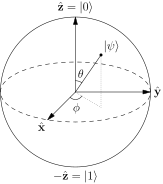
\includegraphics[width=0.2\columnwidth]{Fig/Bloch_Sphere}
\par\end{centering}
\caption{A Bloch-g�mb}
\end{wrapfigure}%
Sz�m�tsuk ki ebben a tiszta �llapotban a s�r�s�g m�trixot:
\begin{equation}
\hat{\rho}=\left|\varphi\right\rangle \left\langle \varphi\right|
\end{equation}
\begin{align}
\hat{\rho} & =\cos^{2}\left(\frac{\theta}{2}\right)\left|\uparrow\right\rangle \left\langle \uparrow\right|+\mathrm{e}^{-\mathrm{i}\phi}\frac{\sin\left(\theta\right)}{2}\left|\uparrow\right\rangle \left\langle \downarrow\right|\\
 & +\mathrm{e}^{\mathrm{i}\phi}\frac{\sin\left(\theta\right)}{2}\left|\downarrow\right\rangle \left\langle \uparrow\right|+\sin^{2}\left(\frac{\theta}{2}\right)\left|\downarrow\right\rangle \left\langle \downarrow\right|
\end{align}
\begin{eqnarray}
\hat{\rho} & = & \left(\begin{array}{cc}
\cos^{2}\left(\frac{\theta}{2}\right) & \mathrm{e}^{-\mathrm{i}\phi}\frac{\sin\left(\theta\right)}{2}\\
\mathrm{e}^{\mathrm{i}\phi}\frac{\sin\left(\theta\right)}{2} & \sin^{2}\left(\frac{\theta}{2}\right)
\end{array}\right)=\frac{1}{2}\left(\begin{array}{cc}
1+\cos\left(\theta\right) & \mathrm{e}^{-\mathrm{i}\phi}\sin\left(\theta\right)\\
\mathrm{e}^{\mathrm{i}\phi}\sin\left(\theta\right) & 1-\cos\left(\theta\right)
\end{array}\right)
\end{eqnarray}
\begin{equation}
\hat{\rho}=\frac{1}{2}\left(\sigma_{0}+\sin\left(\theta\right)\cos\left(\phi\right)\sigma_{x}+\sin\left(\theta\right)\sin\left(\phi\right)\sigma_{y}+\cos\left(\theta\right)\sigma_{z}\right)
\end{equation}
\begin{shaded}%
\begin{equation}
d=\frac{1}{2}\rightarrow\mathrm{Tr}\hat{\rho}=1,\quad\mathrm{Tr}\hat{\rho}^{2}=1
\end{equation}
\end{shaded}

\subsubsection*{b) Teljesen kevert �llapot:}

Hat�rozzuk meg a $\left|\uparrow\right\rangle $ �s $\left|\downarrow\right\rangle $
�llapotok $1/2$ val�sz�n�s�ggel vett statisztikus kever�k�nek s�r�s�g
m�trix�t: 
\begin{align}
\hat{\rho} & =\frac{\left|\uparrow\right\rangle \left\langle \uparrow\right|+\left|\downarrow\right\rangle \left\langle \downarrow\right|}{2},\\
 & =\frac{1}{2}\left(\begin{array}{cc}
1 & 0\\
0 & 1
\end{array}\right)=\frac{\sigma_{0}}{2}.
\end{align}
\begin{shaded}%
\begin{equation}
d=0\rightarrow\mathrm{Tr}\hat{\rho}=1,\quad\mathrm{Tr}\hat{\rho}^{2}=\frac{1}{2}
\end{equation}
\end{shaded}

\subsubsection*{c) R�szlegesen kevert �llapot}

Hat�rozzuk meg a $\left|\uparrow\right\rangle $ �s $\left|\downarrow\right\rangle $
�llapotok $p$ val�sz�n�s�ggel vett statisztikus kever�k�nek s�r�s�g
m�trix�t:
\begin{align}
\hat{\rho} & =p\left|\uparrow\right\rangle \left\langle \uparrow\right|+(1-p)\left|\downarrow\right\rangle \left\langle \downarrow\right|\\
 & =\left(\begin{array}{cc}
p & 0\\
0 & 1-p
\end{array}\right)=\frac{\sigma_{0}}{2}+\left(p-\frac{1}{2}\right)\sigma_{z}
\end{align}
\begin{equation}
d=\left(p-\frac{1}{2}\right)\rightarrow\mathrm{Tr}\hat{\rho}=1,\quad\mathrm{Tr}\hat{\rho}^{2}=\frac{1}{2}+2\left(p-\frac{1}{2}\right)^{2}
\end{equation}
\shadowbox{\begin{minipage}[t]{0.9\columnwidth}%
\begin{xca}
Tekints�k egy k�t �llapot� rendszer k�t ($\left|\alpha\right\rangle $
�s $\left|\beta\right\rangle $) nem ortogon�lis �llapot�b�l ($\left\langle \alpha\right.\left|\beta\right\rangle =x$)
$p$ val�sz�n�s�ggel kevert �llapotot. Hat�rozzuk meg $\mathrm{Tr}\hat{\rho}^{2}$-t
!
\end{xca}
%
\end{minipage}}

\part{�llapot sz�mol�s}

\begin{shaded}%
\textbf{�llapotok sz�ma adott $E$ energia alatt:}

\begin{eqnarray}
\text{Klasszikus rendszer: }\Omega_{0}(E) & = & \frac{1}{h^{N}}\underset{H(\mathbf{p},\mathbf{q})<E}{\int}\left(\mbox{d}p\mbox{d}q\right)^{N}\label{eq:klasszik-Omega-def}\\
\text{Kvantumos rendszer: }\Omega_{0}(E) & = & \sum_{E_{n}<E}1=\sum_{n}\Theta\left(E-E_{N}\right)\label{eq:kvanum-Omega-def}
\end{eqnarray}

\textbf{�llapotok sz�ma $E$ �s $E+\delta E$ k�z�tt:
\begin{equation}
\Omega(E,\delta E)=\Omega_{0}(E+\delta E)-\Omega_{0}(E)
\end{equation}
}

\textbf{�llapots�r�s�g:
\begin{equation}
\omega\left(E\right)=\frac{\mathrm{d}\Omega_{0}}{\mathrm{d}E}=\lim_{\delta E\rightarrow0}\frac{\Omega(E,\delta E)}{\delta E}
\end{equation}
}

\textbf{F�zis t�rfogat elem szab�ly:}

\textbf{
\begin{equation}
h=\mathrm{d}p\mathrm{d}q\label{eq:weyl-szabaly}
\end{equation}
}\end{shaded}Az al�bbiakban h�rom egyszer�en sz�m�that� rendszer �llapotainak sz�m�t
hat�rozzuk meg klasszikus �s kvantumos m�dszerekkel. 

\section{Egy darab, dobozba z�rt, egydimenzi�s r�szecske}

\subsection{Klasszikus}

A Hamilton-f�ggv�ny csak a kinetikus energi�b�l sz�rmaz� tagot tartalmazza:

\begin{equation}
H=\frac{p^{2}}{2m}.
\end{equation}
Egy adott $E$ energia alatti �llapotok a f�zis t�rben egy t�glalapot
jel�lnek ki, melynek fel�lete adja $\Omega_{0}$-t:\begin{wrapfigure}{o}{0.3\columnwidth}%
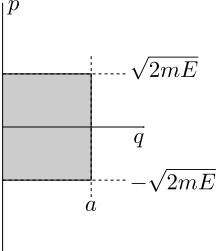
\includegraphics[width=0.2\columnwidth]{Fig/1D_doboz}

\caption{Klasszikus dobozba z�rt r�szecske f�zistere}
\end{wrapfigure}%

\begin{equation}
\Omega_{0}\left(E\right)=\underset{H<E}{\int}\frac{\mathrm{d}p\mathrm{d}q}{h}=\frac{2a}{h}\sqrt{2mE}.
\end{equation}


\subsection{Kvantumos}

A kvantummechanikai le�r�s a Schr�dinger-egyenlet megold�s�val kezd�dik.

\begin{eqnarray}
-\frac{\hbar^{2}}{2m}\partial_{x}^{2}\psi & = & E\psi,\\
\psi_{k}^{\infty}(x) & = & \mbox{e}^{\mbox{i}kx},\\
E & = & \frac{\hbar^{2}k^{2}}{2m},\\
k & = & \frac{\sqrt{2mE}}{\hbar}.
\end{eqnarray}
Itt feltett�k hogy egy v�gtelen rendszert vizsg�lunk. A v�ges rendszer
�llapotait illetve spektrum�t a v�gtelen rendszerb�l a megfelel� peremfelt�telek
kirov�s�val �s azok teljes�t�s�vel kapjuk. Vizsg�ljuk meg a k�t leggyakrabban
t�rgyalt peremfelt�telt!

\subsubsection*{a) Z�rt peremfelt�tel}

\begin{equation}
\psi\left(0\right)=\psi\left(a\right)=0.
\end{equation}
\begin{wrapfigure}{o}{0.3\columnwidth}%
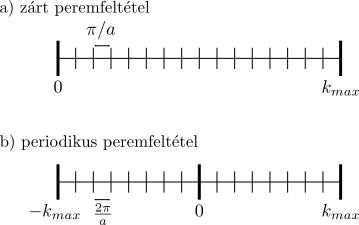
\includegraphics[width=0.3\columnwidth]{Fig/1D_doboz_q_kter}

\caption{Kvantumos dobozba z�rt r�szecske hull�msz�mt�rben}
\end{wrapfigure}%

Adott $E$ energi�n a z�rt peremfelt�telt teljes�t� hull�mf�ggv�ny
el��ll mint a $k$ �s a $-k$ hull�msz�mokhoz tatoz� hull�mf�ggv�nyek
line�rkombin�ci�ja: 
\begin{equation}
\psi_{k}^{\text{z�rt}}\left(x\right)=\frac{\psi_{k}^{\infty}\left(x\right)-\psi_{-k}^{\infty}\left(x\right)}{2\mathrm{i}}=\sin\left(kx\right)
\end{equation}
A peremfelt�tel megk�ti a $k$ hull�msz�m lehets�ges �rt�k�t:
\begin{eqnarray}
\psi(a) & = & 0\rightarrow k=\frac{n\pi}{a},\quad n=1,2,\dots n_{max},\\
 &  & k_{max}=\frac{n_{max}\pi}{a},\\
 &  & E_{max}=\frac{\hbar^{2}}{2m}\left(\frac{n_{max}\pi}{a}\right)^{2}.
\end{eqnarray}
Adott $E$energia alatt l�v� �llapotok sz�ma teh�t
\begin{equation}
\Omega_{0}\left(E\right)=\mathrm{Int}\left[\frac{a}{\pi\hbar}\sqrt{2mE}\right]=\mathrm{Int}\left[\frac{2a}{h}\sqrt{2mE}\right]
\end{equation}
ahol bevezett�k a $\mathrm{Int}\left[x\right]$ jel�l�st $x$ val�s
sz�m eg�sz r�sz�re.\begin{wrapfigure}{o}{0.3\columnwidth}%
\begin{centering}
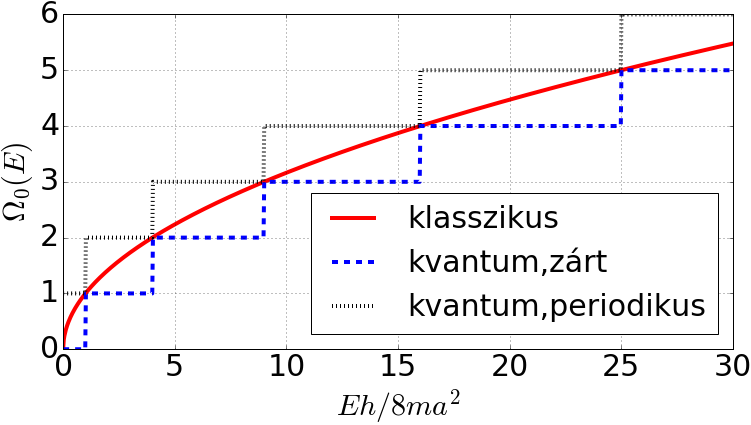
\includegraphics[width=0.3\textwidth]{Fig/1d_doboz_Omega}
\par\end{centering}
\caption{Dobozba z�rt r�szecske �llapotainak sz�ma\label{fig:1d-doboz-omega}}
\end{wrapfigure}%


\subsubsection*{b) Periodikus peremfelt�tel}

Ha periodikus peremfelt�tellel �l�nk akkor a v�gtelen rendszer s�khull�m
megold�sai megfelel� $k$ hull�msz�mok mellett m�r kiel�g�t� megold�sai
a Schr�dinger egyenletnek: 
\begin{equation}
\psi_{k}^{\text{periodikus}}\left(x\right)=\psi_{k}^{\infty}(x)=\mbox{e}^{\mbox{i}kx},
\end{equation}
\begin{eqnarray}
\psi\left(x+a\right) & = & \psi\left(x\right),\\
 &  & \rightarrow\mbox{e}^{\mbox{i}kx}=\mbox{e}^{\mbox{i}kx+\mbox{i}ka}\\
 &  & \rightarrow ka=2n\pi\\
 &  & n=-n_{max}\dots0\dots n_{max}
\end{eqnarray}
Adott $E$energia alatt l�v� �llapotok sz�ma teh�t
\begin{equation}
\Omega_{0}\left(E\right)=2\mathrm{Int}\left[\frac{a}{2\pi}\frac{\sqrt{2mE}}{\hbar}\right]+1=2\mathrm{Int}\left[\frac{a}{h}\sqrt{2mE}\right]+1
\end{equation}
Mindk�t peremfelt�tel eset�n teljes�l teh�t hogy nagy energi�kra a
klasszikus �llapotsz�m j� k�zel�t�se a kvantumos kifejez�seknek.

\newpage{}

\section{Rot�tor}

\begin{wrapfigure}{o}{0.3\columnwidth}%
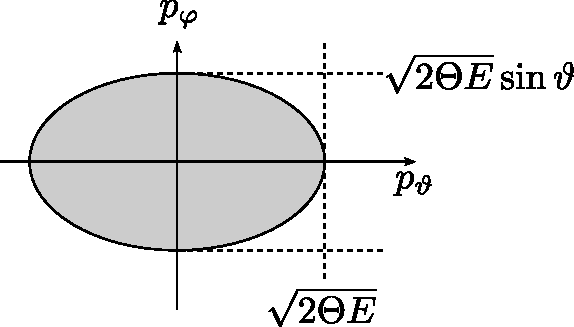
\includegraphics[width=0.3\columnwidth]{Fig/rotator_phase_space}

\caption{A rot�tor f�zister�nek impulzus altere}
\end{wrapfigure}%
A rot�tor egy egy t�rbeli t�megpont melynek $r$ t�vols�ga a koordin�ta
rendszer k�z�ppontj�t�l id�ben �lland�, azaz 
\begin{equation}
\frac{\mathrm{d}}{\mathrm{d}t}r=\dot{r}=0.
\end{equation}


\subsection{Klasszikus}

Fejezz�k ki a poz�ci� �s a sebess�g vektorokat \href{https://en.wikipedia.org/wiki/Spherical_coordinate_system}{g�mbi pol�rkoordin�ta rendszerben }

\begin{equation}
\vec{r}=\left(\begin{array}{c}
x\\
y\\
z
\end{array}\right)=r\left(\begin{array}{c}
\sin\vartheta\cos\varphi\\
\sin\vartheta\sin\varphi\\
\cos\vartheta
\end{array}\right),\quad\dot{\vec{r}}=r\left(\begin{array}{c}
\dot{\vartheta}\cos\vartheta\cos\varphi-\dot{\varphi}\sin\vartheta\sin\varphi\\
\dot{\vartheta}\cos\vartheta\sin\varphi+\dot{\varphi}\sin\vartheta\cos\varphi\\
-\dot{\vartheta}\sin\vartheta
\end{array}\right)
\end{equation}
A sebess�g n�gyzete teh�t

\begin{eqnarray}
\dot{x}^{2} & = & r^{2}\left(\dot{\vartheta}^{2}\cos^{2}\vartheta\cos^{2}\varphi+\dot{\varphi}^{2}\sin^{2}\vartheta\sin^{2}\varphi-\frac{\dot{\vartheta}\dot{\varphi}\sin\left(2\vartheta\right)\sin\left(2\varphi\right)}{2}\right),\nonumber \\
\dot{y}^{2} & = & r^{2}\left(\dot{\vartheta}^{2}\cos^{2}\vartheta\sin^{2}\varphi+\dot{\varphi}^{2}\sin^{2}\vartheta\cos^{2}\varphi+\frac{\dot{\vartheta}\dot{\varphi}\sin\left(2\vartheta\right)\sin\left(2\varphi\right)}{2}\right),\\
\dot{z}^{2} & = & r^{2}\dot{\vartheta}^{2}\sin^{2}\vartheta.\nonumber 
\end{eqnarray}
\begin{equation}
\left(\dot{x}^{2}+\dot{y}^{2}+\dot{z}^{2}\right)=r^{2}\left[\dot{\vartheta}^{2}\underbrace{\left(\cos^{2}\vartheta\cos^{2}\varphi+\cos^{2}\vartheta\sin^{2}\varphi+\sin^{2}\vartheta\right)}_{1}+\dot{\varphi}^{2}\overbrace{\left(\sin^{2}\vartheta\sin^{2}\varphi+\sin^{2}\vartheta\cos^{2}\varphi\right)}^{\sin^{2}\vartheta}\right].
\end{equation}
A kinetikus energia sz�gv�ltoz�kkal kifejezve a k�vetkez� alakot �lti
\begin{eqnarray}
E_{kin} & = & \frac{1}{2}m\left(\dot{x}^{2}+y^{2}+\dot{z}^{2}\right),\\
 & = & \frac{1}{2}mr^{2}\left[\dot{\vartheta}^{2}+\dot{\varphi}^{2}\sin^{2}\vartheta\right],\\
 & = & \frac{1}{2}\Theta\left[\dot{\vartheta}^{2}+\dot{\varphi}^{2}\sin^{2}\vartheta\right].
\end{eqnarray}
A Lagrange-f�ggv�ny szok�sos deriv�ltjaib�l a sz�gv�ltoz�khoz konjug�lt
impulzusok 
\begin{equation}
\mathcal{L}=E_{kin},\rightarrow p_{\vartheta}=\frac{\partial\mathcal{L}}{\partial\dot{\vartheta}}=\Theta\dot{\vartheta},\quad p_{\varphi}=\frac{\partial\mathcal{L}}{\partial\dot{\varphi}}=\Theta\sin^{2}\vartheta\dot{\varphi},
\end{equation}
�s a Hamilton-f�ggv�ny pedig 

\begin{equation}
H=E_{kin}=\frac{1}{2\Theta}\left(p_{\vartheta}^{2}+\frac{p_{\varphi}^{2}}{\sin^{2}\vartheta}\right).\label{eq:rotator-hamilton-klasszik}
\end{equation}
Adott $E$ energia alatti �llapotok sz�ma az impulzus alt�rben egy
ellipszis ter�let�nek sz�m�t�s�val illetve a koordin�t�kban egy g�mb
fel�let�nek sz�m�t�s�val kaphat� meg 
\begin{eqnarray}
\Omega_{0}(E) & = & \frac{1}{h^{2}}\int_{H<E}\mathrm{d}\vartheta\mathrm{d}\varphi\mathrm{d}p_{\vartheta}\mathrm{d}p_{\varphi},\\
 & = & \frac{1}{h^{2}}\pi\sqrt{2E\Theta}\sqrt{2E\Theta}\underbrace{\int_{0}^{2\pi}\int_{0}^{\pi}\sin\vartheta\mathrm{d}\vartheta\mathrm{d}\varphi}_{\text{"t�rsz�g"}=4\pi},
\end{eqnarray}
\begin{equation}
\Omega_{0}(E)=\frac{2\Theta E}{\hbar^{2}}.
\end{equation}


\subsection{Kvantumos}

A kvantumos le�r�shoz egy forg� test \href{https://en.wikipedia.org/wiki/Rigid_rotor}{Hamilton-oper�tor�b�l}
indulunk ki:

\begin{equation}
\hat{H}=\frac{\left(\hat{\vec{r}}\times\hat{\vec{p}}\right)\cdot\left(\hat{\vec{r}}\times\hat{\vec{p}}\right)}{2\Theta}=\frac{\hat{\vec{L}}^{2}}{2\Theta}.
\end{equation}
\begin{wrapfigure}{o}{0.3\columnwidth}%
\begin{centering}
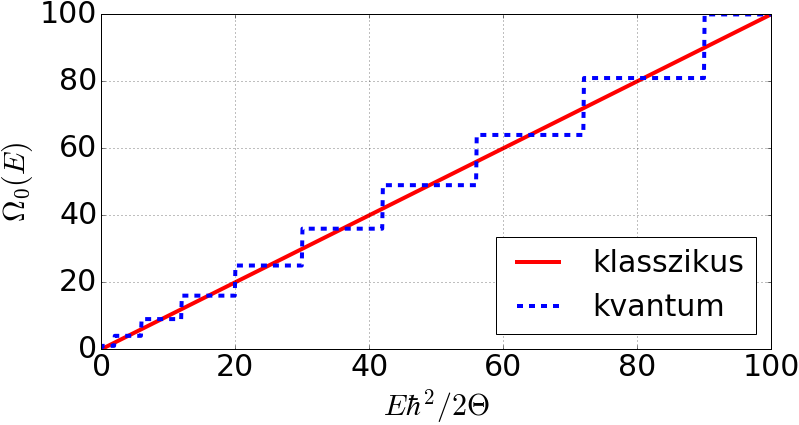
\includegraphics[width=0.3\columnwidth]{Fig/rotator_Omega}
\par\end{centering}
\caption{A klasszikus �s kvantumos rot�tor �llapotainak sz�ma}
\end{wrapfigure}%
Ennek az oper�tornak a spektruma
\begin{equation}
E_{l}=\frac{\hbar^{2}l(l+1)}{2\Theta}.\label{eq:rotator-kvantum-spektrum}
\end{equation}
Egy adott $E$ energia �s az alatta l�v� legnagyobb impulzus momentum
�rt�k $l_{max}$ kapcsolata teh�t
\begin{equation}
l_{max}(l_{max}+1)=\mathrm{Int}\left[\frac{2\Theta E}{\hbar^{2}}\right].
\end{equation}
Mivel minden $l$ �llapot $\left(2l+1\right)$-szeresen degener�lt
ez�rt az adott $E$ energia alatti �llapotok �sszege el��ll p�ratlan
sz�mok �sszegek�nt: 
\begin{equation}
\Omega_{0}(E)=\sum_{l=0}^{l_{max}}\left(2l+1\right)=(l_{max}+1)^{2}.
\end{equation}
A klasszikus kifejez�st visszakapjuk ha $l_{max}\gg1\rightarrow l_{max}(l_{max}+1)\approx(l_{max}+1)^{2}$,
ekkor
\begin{equation}
\Omega_{0}(E)\approx\frac{2\Theta E}{\hbar^{2}}.
\end{equation}


\section{Harmonikus oszcill�tor}

A harmonikus oszcill�tor (�s a hidrog�n atom ...) sok szempontb�l
az elm�leti sz�m�t�sok �llatorvosi lova. Hat�rozzuk meg az �llapotok
sz�m�t ebben az egyszer� rendszerben is.

\subsection{Klasszikus}

A Hamilton-f�ggv�ny alakj�b�l 

\begin{equation}
H=\frac{p^{2}}{2m}+\frac{1}{2}m\omega^{2}q^{2},
\end{equation}
\begin{wrapfigure}{o}{0.3\columnwidth}%
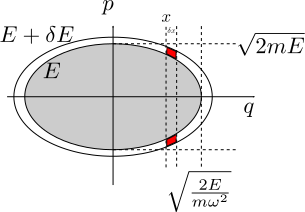
\includegraphics[width=0.3\columnwidth]{Fig/oscillator_phase_space}

\caption{Az oszcill�tor f�zistere}
\end{wrapfigure}%
j�l l�tszik hogy egy adott $E$ energia egy ellipszist hat�roz meg,
azaz az �llapotok sz�ma 
\begin{equation}
\Omega_{0}(E)=\frac{1}{h}\int_{H<E}\mathrm{d}p\mathrm{d}q=\frac{1}{h}\sqrt{2mE}\sqrt{\frac{2E}{m\omega^{2}}}\pi,
\end{equation}
\begin{equation}
\Omega_{0}(E)=\frac{E}{\hbar\omega}.\label{eq:harmonikus-oszci-omega0}
\end{equation}


\subsection{Kvantumos}

A kvantumos �llapotsz�mol�shoz induljunk ki a harmonikus oszcill�tor
spektrum�b�l:

\begin{equation}
E_{n}=\hbar\omega\left(n+\frac{1}{2}\right),\quad n=0,1,2\dots
\end{equation}

\begin{wrapfigure}{o}{0.3\columnwidth}%
\begin{centering}
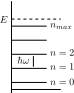
\includegraphics[height=0.2\columnwidth]{Fig/oscillator_spectrum}
\par\end{centering}
\caption{Az oszcill�tor spektruma}
\end{wrapfigure}%

Azaz egy adott $E$ energia alatt az $n$ index maxim�lis �rt�ke
\begin{equation}
n_{max}=\mathrm{Int}\left[\frac{E}{\hbar\omega}-\frac{1}{2}\right],
\end{equation}
amib�l
\begin{eqnarray}
\Omega_{0} & (E)=\mathrm{Int}\left[\frac{E}{\hbar\omega}-\frac{1}{2}\right] & +1=\mathrm{Int}\left[\frac{E}{\hbar\omega}+\frac{1}{2}\right].
\end{eqnarray}
Itt is l�tjuk hogy nagy energi�kra vagy a $\hbar\rightarrow0$ hat�resetben
a klasszikus �s a kvantumos �llapotsz�m megegyezik.

\subsection{Egy �rdekes feladat}

Mikrokanonikus sokas�got felt�telezve l�ssuk be hogy annak a val�sz�n�s�ge
hogy egy klasszikus harmonikus oszcill�tor helyzete $x$ �s $x+\delta x$
k�z�tt van, $P(x,x+\delta x)$, megegyezik az oszcill�tor ezen intervallumban
elt�lt�tt ideje, $t(x,x+\delta x)$, �s a peri�dus id�, $T_{per}=\frac{2\pi}{\omega}$,
h�nyados�val: 
\begin{equation}
P(x,x+\delta x)=\frac{t(x,x+\delta x)}{T_{per}}
\end{equation}
A k�rd�ses tartom�nyban t�lt�tt id� a tartom�ny hossz�val egyenesen
a tartom�nyon t�rt�n� �thalad�s sebess�g�vel viszont ford�tottan ar�nyos.
Az ar�nyoss�gi t�nyez� $2$ hiszen odafele �s visszafele is id�z�nk
$x$ k�zel�ben! 
\begin{equation}
t(x,x+\delta x)=2\frac{\delta x}{v(x)}.
\end{equation}
A vizsg�lt $P(x,x+\delta x)$ val�sz�n�s�g a megfelel� f�zist�r t�rfogatok
ar�ny�val kifejezve: 
\begin{equation}
P(x,x+\delta x)=\frac{2\mathrm{d}p(x)\delta x/h}{\Omega\left(E,\delta E\right)}=\frac{2\frac{\mathrm{d}p(x)}{\mathrm{d}E}\delta E\delta x/h}{\Omega\left(E,\delta E\right)}\label{eq:harmonikus-oszci-Pxpdx}
\end{equation}
Felhaszn�lva $\Omega$ defin�ci�j�t (\ref{eq:klasszik-Omega-def})
�s a harmonikus oszcill�tor �llapotainak sz�m�t (\ref{eq:harmonikus-oszci-omega0})
kapjuk, hogy 
\begin{equation}
\Omega\left(E,\delta E\right)=\frac{\mathrm{d}\Omega_{0}}{\mathrm{d}E}\delta E=\frac{2\pi}{h\omega}\delta E.
\end{equation}
Felhaszn�lva a harmonikus oszcill�tor energi�j�t 
\begin{equation}
E=\frac{p^{2}}{2m}+\frac{1}{2}m\omega^{2}x^{2}=\frac{mv^{2}}{2}+\frac{1}{2}m\omega^{2}x^{2},
\end{equation}
a$\mathrm{d}p/\mathrm{d}E$ deriv�lt (tal�n nem t�l meglep� m�don)
\begin{equation}
\frac{1}{\frac{\mathrm{d}p}{\mathrm{d}E}}=\frac{\mathrm{d}E}{\mathrm{d}p}=\frac{p}{m}=v.
\end{equation}
A fentieket visszahelyettes�tve (\ref{eq:harmonikus-oszci-Pxpdx})-be
kapjuk, hogy 
\begin{equation}
P(x,x+\delta x)=\frac{2\frac{1}{v}\delta E\delta x/h}{\frac{2\pi}{h\omega}\delta E}=2\frac{\frac{\delta x}{v}}{\frac{2\pi}{\omega}}=\frac{t(x,x+\delta x)}{T_{per}}.
\end{equation}
\href{https://en.wikipedia.org/wiki/Q.E.D.}{q.e.d} (nem kvantum elektrodinamika...)

\shadowbox{\begin{minipage}[t]{0.9\columnwidth}%
\begin{xca}
Hat�rozzuk meg a klasszikus �llapotok $\Omega_{0}$ sz�m�t adott $E$
energia alatt a k�vetkez� rendszerekre!
\end{xca}
\begin{enumerate}
\item Pattog� labda
\begin{equation}
H=\frac{p^{2}}{2m}+gx,\quad x\ge0
\end{equation}
\item Relativisztikus oszcill�tor
\begin{equation}
H=c\left|p\right|+\frac{1}{2}\alpha\omega^{2}x^{2},
\end{equation}
\item Relativisztikus pattog� labda
\begin{equation}
H=c\left|p\right|+gx,x\ge0
\end{equation}
\end{enumerate}
%
\end{minipage}}\newpage{}

\part{Termodinamikai mennyis�gek mikrokanonikus sokas�gb�l}

Ebben a fejezetben a mikrokanonikus formalizmus seg�ts�g�vel n�h�ny
alapvet� modell rendszer termodinamikai mennyis�geinek sz�rmaztat�s�t
fogjuk vizsg�lni.%
\begin{shaded}%
\textbf{Entr�pia:}

Ha a rendszer energi�ja $E$ �s $E$ �s $E+\delta E$ k�z�tt az �llapotok
sz�ma $\Omega$ akkor a rendszer entr�pi�ja:\textbf{
\begin{equation}
S=k_{\mathrm{B}}\ln\Omega(E,\delta E)
\end{equation}
}

Termodinamikai hat�resetben haszn�lhat� feltev�s:
\begin{equation}
S=k_{\mathrm{B}}\ln\Omega(E,\delta E)=k_{\mathrm{B}}\ln\omega(E)\delta E=k_{\mathrm{B}}\ln\Omega_{0}(E)\label{eq:entropia-praktice}
\end{equation}

\textbf{Fundament�lis egyenlet:}

\begin{equation}
\mathrm{d}E=T\mathrm{d}S-p\mathrm{d}V+\mu\mathrm{d}N\label{eq:mikro-fundamental}
\end{equation}

\textbf{H�m�rs�klet:}

\begin{equation}
\frac{1}{T}=\left.\frac{\partial S}{\partial E}\right|_{V,N}\label{eq:homerseklet}
\end{equation}

\textbf{Nyom�s:}
\begin{equation}
\frac{p}{T}=\left.\frac{\partial S}{\partial V}\right|_{E,N}\label{eq:nyomas}
\end{equation}

\textbf{K�miai potenci�l:}
\begin{equation}
\frac{\mu}{T}=-\left.\frac{\partial S}{\partial N}\right|_{E,V}\label{eq:kemiai-potencial}
\end{equation}

\textbf{H�kapacit�s:}
\begin{equation}
C=\left.\frac{\partial E}{\partial T}\right|_{V}\label{eq:fajho}
\end{equation}
\end{shaded}

\section{$N$ darab k�t �llapot� rendszer}

\begin{wrapfigure}{o}{0.3\columnwidth}%
\centering{}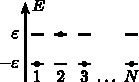
\includegraphics[height=0.1\columnwidth]{Fig/N2all_setup}\caption{$N$ darab k�t �llapot� rendszer }
\end{wrapfigure}%

Vizsg�ljunk egy olyan $N$ r�szecsk�b�l �ll� rendszert amelyben egy
adott r�szecske energi�ja vagy $\varepsilon$ vagy $-\varepsilon$.
Gondolhatunk itt p�ld�ul egy klasszikus k�t �llapot� spin rendszerre,
vagy valamilyen adatt�rol�ban klasszikus bitekre! Jel�lje $N_{+}$az
$\varepsilon$ energi�j� r�szecsk�k sz�m�t illetve $N_{-}$ a $-\varepsilon$
energi�j� r�szecsk�k sz�m�t. Term�szetesen\inputencoding{latin9}\foreignlanguage{english}{
\begin{equation}
N=N_{+}+N_{-}.
\end{equation}
}

\inputencoding{latin2}A rendszer teljes $E$ energi�ja �rtelemszer�en 

\begin{equation}
E=\left(N_{+}-N_{-}\right)\varepsilon=M\varepsilon,\quad M=-N,-N+2,\dots N
\end{equation}
Ahol bevezett�k az $M$ v�ltoz�t amire gondolhatunk �gy mint a rendszer
``m�gnesezetts�ge''. 
\begin{eqnarray}
N & = & N_{+}+N_{-},\quad N_{+}=\frac{N+M}{2}\\
M & = & N_{+}-N_{-},\quad N_{-}=\frac{N-M}{2}
\end{eqnarray}
H�ny olyan konfigur�ci� van amely energi�ja $E=M\varepsilon$? M�sf�lek�ppen
h�nyf�le m�don tudunk kiv�lasztani $N$ fels� szintb�l $N_{+}$-at
? 
\begin{equation}
\Omega\left(E,\delta E\right)=\left(\begin{array}{c}
N\\
N_{+}
\end{array}\right)=\frac{N!}{N_{+}!\left(N-N_{+}\right)!}=\frac{N!}{N_{+}!N_{-}!}
\end{equation}
Az �llapotok sz�m�nak ismeret�ben az entr�pia (\ref{eq:entropia-praktice})-nak
megfelel�en
\begin{equation}
S=k_{\mathrm{B}}\ln\Omega=k_{\mathrm{B}}\left(\ln N!-\ln N_{+}!-\ln N_{-}!\right).
\end{equation}
Termodinamikai hat�resetben $N\rightarrow\infty$, $E/N=\mathrm{const.}$
azaz $M/N=\mathrm{const.}$ Ebben a hat�resetben alkalmazhatjuk a
(\ref{eq:stirling-log}) Stirling-formul�t! Elhanyagolva a $\ln N$-es
j�rul�kokat:
\begin{equation}
\ln N!\approx N\ln N-N
\end{equation}
\begin{wrapfigure}{o}{0.3\columnwidth}%
\begin{centering}
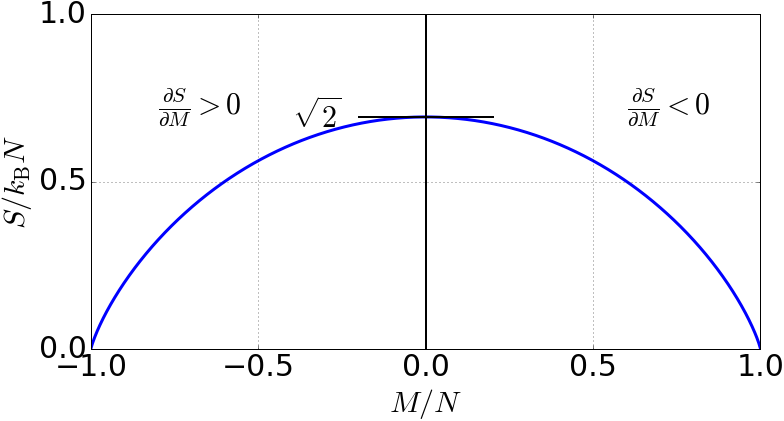
\includegraphics[width=0.3\columnwidth]{Fig/N2all_entropia}
\par\end{centering}
\centering{}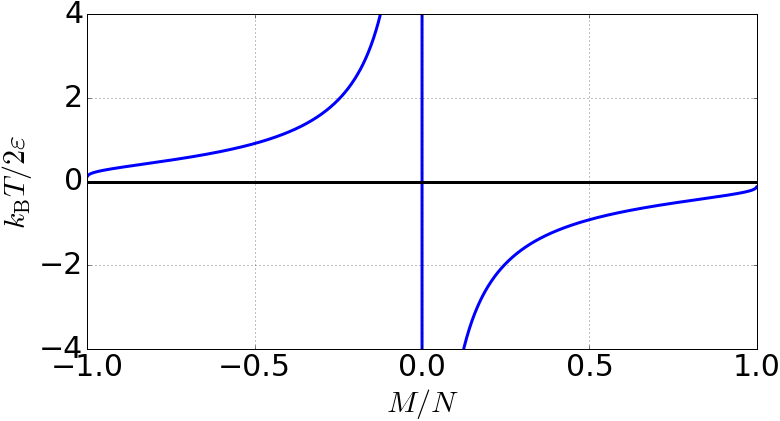
\includegraphics[clip,width=0.3\columnwidth]{Fig/N2all_homerseklet}\caption{$N$ darab k�t �llapot� rendszer entr�pi�ja �s h�m�rs�klete}
\end{wrapfigure}%
\begin{eqnarray}
\frac{S}{k_{\mathrm{B}}} & = & N\ln N-N-N_{+}\ln N_{+}+N_{+}-N_{-}\ln N_{-}+N_{-}\\
 & = & \left(N_{+}+N_{-}\right)\ln N-N_{+}\ln N_{+}-N_{-}\ln N_{-}\nonumber \\
 & = & -N_{+}\ln\frac{N_{+}}{N}-N_{-}\ln\frac{N_{-}}{N}\nonumber \\
 & = & -\frac{N+M}{2}\ln\frac{N+M}{2N}-\frac{N-M}{2}\ln\frac{N-M}{2N}\nonumber \\
S & = & -k_{\mathrm{B}}N\left[\frac{1+m}{2}\ln\frac{1+m}{2}+\frac{1-m}{2}\ln\frac{1-m}{2}\right],\label{eq:N2all-entropia}\\
m & = & \frac{M}{N}=\frac{E}{\varepsilon N}\nonumber 
\end{eqnarray}
Ha $m=0$ azaz azok az �llapotok amelyekben ugyan annyi a$+\varepsilon$
energi�j� �llapot mint a $-\varepsilon$ energi�j� �llapot akkor 
\begin{equation}
S=k_{\mathrm{B}}N\ln2=k_{\mathrm{B}}\ln2^{N}
\end{equation}
ami v�rhat� hiszen ekkor $\Omega=2^{n}$. �rdemes megjegyezni hogy
az entr�pia energia szerinti deriv�ltja csak negat�v energi�kra pozit�v
mennyis�g! Pozit�v energi�kra viszont negat�v azaz ezen a tartom�nyon
a h�m�rs�klet negat�v! Ez a rendszer teh�t termodinamikai �rtelemben
nem ``norm�l'' rendszer! Hasonl� viselked�st mutat minden olyan
rendszer melynek lehets�ges energi�i korl�tos tartom�nyra szor�tkoznak. 

Az entr�pia ismeret�ben a h�m�rs�klet 
\begin{eqnarray}
\frac{1}{T} & = & \left.\frac{\partial S}{\partial E}\right|_{V,N}=\frac{\partial S}{\partial m}\frac{\partial m}{\partial E}=\frac{1}{\varepsilon N}\frac{\partial S}{\partial m}.
\end{eqnarray}
Felhaszn�lva hogy
\begin{equation}
\frac{\partial}{\partial x}(1+px)\ln(1+px)=p\left[\ln(1+px)+1\right],
\end{equation}
\begin{eqnarray}
\frac{1}{T} & = & \frac{1}{\varepsilon N}\frac{\partial S}{\partial m}\\
 & = & -\frac{k_{\mathrm{B}}}{\varepsilon}\frac{\partial}{\partial m}\left[\frac{1+m}{2}\ln\frac{1+m}{2}+\frac{1-m}{2}\ln\frac{1-m}{2}\right]\\
 & = & -\frac{k_{\mathrm{B}}}{2\varepsilon}\frac{\partial}{\partial m}\left[\left(1+m\right)\ln\left(1+m\right)+\left(1-m\right)\ln\left(1-m\right)-2\ln2\right]\\
 & = & -\frac{k_{\mathrm{B}}}{2\varepsilon}\left[\ln\left(1+m\right)+1-\ln\left(1-m\right)-1\right]
\end{eqnarray}
 kapjuk, hogy
\begin{eqnarray}
\frac{1}{T} & = & \frac{k_{\mathrm{B}}}{2\varepsilon}\ln\frac{1-m}{1+m}.\label{eq:N2all-homerseklet}
\end{eqnarray}
A h�m�rs�klet, ahogy azt v�rjuk, intenz�v mennyis�g hiszen $E/N$
f�ggv�nye. �rdemes megjegyezni hogy az entr�pia deriv�ltja $m=\pm1$
eset�n tart $\mp\infty$-hez. Ennek megfelel�en a h�m�rs�klet mind
k�t esetben z�rushoz tart. Exponencializ�lva a fenti \ref{eq:N2all-homerseklet}
kifejez�st 
\begin{equation}
\mbox{e}^{2x}=\frac{1-m}{1+m},\,x=\frac{\varepsilon}{k_{\mathrm{B}}T}.
\end{equation}
Kifejezve $m$-et 
\begin{equation}
m=\frac{1-\mbox{e}^{2x}}{1+\mbox{e}^{2x}}=\frac{\mbox{e}^{-x}-\mbox{e}^{x}}{\mbox{e}^{-x}+\mbox{e}^{x}}=-\tanh\left(x\right),
\end{equation}
a h�m�rs�klet �s a rendszer energi�ja k�z�tt az al�bbi kapcsolatot
�llap�thatjuk meg: 
\begin{equation}
E=-\varepsilon N\tanh\left(\frac{\varepsilon}{k_{\mathrm{B}}T}\right).\label{eq:N2all-energia}
\end{equation}
Hasonl�an a pozit�v illetve negat�v energi�j� ``r�szecsk�k sz�ma'':
\begin{eqnarray}
N_{+} & = & \frac{N+M}{2}=N\frac{\mbox{e}^{-\frac{\varepsilon}{k_{\mathrm{B}}T}}}{\mbox{e}^{-\frac{\varepsilon}{k_{\mathrm{B}}T}}+\mbox{e}^{\frac{\varepsilon}{k_{\mathrm{B}}T}}},\\
N_{-} & = & \frac{N-M}{2}=N\frac{\mbox{e}^{\frac{\varepsilon}{k_{\mathrm{B}}T}}}{\mbox{e}^{-\frac{\varepsilon}{k_{\mathrm{B}}T}}+\mbox{e}^{\frac{\varepsilon}{k_{\mathrm{B}}T}}}.
\end{eqnarray}
A h�kapacit�s a (\ref{eq:fajho}) szerint 
\begin{eqnarray}
C & = & \left.\frac{\partial E}{\partial T}\right|_{V}=\frac{\partial E}{\partial x}\frac{\partial x}{\partial T}=-\frac{\varepsilon}{k_{\mathrm{B}}T^{2}}\frac{\partial E}{\partial x}\\
 & = & \frac{\varepsilon^{2}N}{k_{\mathrm{B}}T^{2}}\frac{\partial\tanh\left(x\right)}{\partial x}=k_{\mathrm{B}}N\frac{x^{2}}{\cosh^{2}x},\\
 & = & k_{\mathrm{B}}N\frac{\left(\frac{\varepsilon}{k_{\mathrm{B}}T}\right)^{2}}{\cosh^{2}\left(\frac{\varepsilon}{k_{\mathrm{B}}T}\right)}.
\end{eqnarray}
A h�kapacit�s alacsony illetve magas h�m�rs�klet� viselked�s�re a
$\cosh$ f�ggv�ny tulajdons�gaib�l k�vetkeztethet�nk. Alacsony h�m�rs�kleten,
azaz $x\rightarrow\infty$
\begin{equation}
\cosh x=\frac{\mbox{e}^{x}+\mbox{e}^{-x}}{2}\underset{x\rightarrow\infty}{=}\frac{\mbox{e}^{x}}{2},
\end{equation}
m�g magas h�m�rs�kleten azaz \inputencoding{latin9}\foreignlanguage{english}{$x\rightarrow0$}\inputencoding{latin2}
\begin{equation}
\lim_{x\rightarrow0}\cosh x=1.
\end{equation}
Ezen �sszef�gg�sek seg�ts�g�vel: \begin{wrapfigure}{o}{0.3\columnwidth}%
\centering{}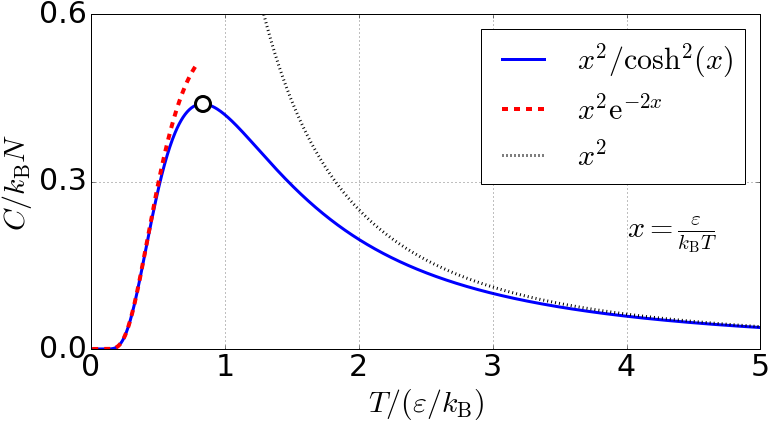
\includegraphics[width=0.3\columnwidth]{Fig/N2all_hokapacitas}\caption{$N$ darab k�t �llapot� rendszer h�kapacit�sa}
\end{wrapfigure}%
\begin{eqnarray}
T & \rightarrow & 0,x\rightarrow\infty,\quad C\rightarrow k_{\mathrm{B}}N\left(\frac{2\varepsilon}{k_{\mathrm{B}}T}\right)^{2}\mbox{e}^{-\frac{2\varepsilon}{k_{\mathrm{B}}T}},\\
T & \rightarrow & \infty,x\rightarrow0,\quad C\rightarrow\frac{N\varepsilon^{2}}{k_{\mathrm{B}}T^{2}}.
\end{eqnarray}
Amint azt az �bra is mutatja a fajh� h�m�rs�klet f�gg�se maxim�lis
egy adott h�m�rs�klet �rt�kn�l. Hat�rozzuk meg ezt a H�m�rs�klet �rt�ket!
\begin{equation}
\partial_{x}C\propto\partial_{x}\left(\frac{x^{2}}{\cosh^{2}x}\right)=\frac{2x}{\cosh^{2}x}-\frac{x^{2}2\sinh x}{\cosh^{3}x}=\frac{2x\left(1-x\tanh x\right)}{\cosh^{2}x}
\end{equation}
A deriv�lt k�t helyen v�lik z�russ� $x=0$-ban illetve $x=x_{max}$-n�l
ahol 
\begin{equation}
1-x_{max}\tanh x_{max}=0.
\end{equation}
Az egyenletet numerikusan megoldva $x_{max}\approx1.199$, $x_{max}^{-1}\approx0.8335$. 

Vizsg�ljuk meg most a rendszerb�l kiszemelt egy alrendszer statisztik�j�t.
Mi a val�sz�n�s�ge hogy az 1. rendszer a $+\varepsilon$ �llapotban
van, ha a rendszer adott $E=\varepsilon M$ energi�n van? 
\begin{equation}
P_{1}^{+}=\frac{\left(N-1\right)!}{\left(N_{+}-1\right)!N_{-}!}\frac{N_{+}!N_{-}!}{N!}=\frac{N_{+}}{N}=\frac{\mbox{e}^{-\frac{\varepsilon}{k_{\mathrm{B}}T}}}{\mbox{e}^{-\frac{\varepsilon}{k_{\mathrm{B}}T}}+\mbox{e}^{\frac{\varepsilon}{k_{\mathrm{B}}T}}}.
\end{equation}
Hasonl� megfontol�sok alapj�n annak a val�sz�n�s�ge hogy az 1. rendszer
a $-\varepsilon$ �llapotban van:
\begin{equation}
P_{1}^{-}=\frac{\mbox{e}^{\frac{\varepsilon}{k_{\mathrm{B}}T}}}{\mbox{e}^{-\frac{\varepsilon}{k_{\mathrm{B}}T}}+\mbox{e}^{\frac{\varepsilon}{k_{\mathrm{B}}T}}}.
\end{equation}
A k�t val�sz�n�s�g h�nyadosa

\begin{equation}
\frac{P_{1}^{+}}{P_{1}^{-}}=\mbox{e}^{-\frac{2\varepsilon}{k_{\mathrm{B}}T}}.
\end{equation}
Amint k�s�bb l�tni fogjuk, a kanonikus sokas�g terminol�gi�it haszn�lva
pontosan ugyan ezek a val�sz�n�s�gi s�lyok fogj�k jellemezni a rendszert.

\section{$N$ darab harmonikus oszcill�tor}

A m�sodik p�ld�ban vizsg�ljunk meg $N$ darab harmonikus oszcill�tort.
A rendszer Hamilton-oper�tora: 

\begin{equation}
\hat{H}=\sum_{i=1}^{N}\frac{\hat{p}_{i}^{2}}{2m}+\frac{1}{2}m\omega^{2}\hat{x}_{i}^{2}
\end{equation}

\begin{wrapfigure}{o}{0.3\columnwidth}%
\centering{}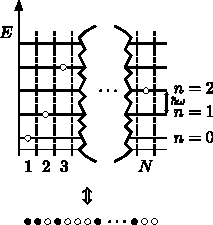
\includegraphics[width=0.3\columnwidth]{Fig/Noscillator_spectrum}\caption{$N$ oszcill�tor rendszer }
\end{wrapfigure}%
A rendszer teljes energi�ja a r�szrendszerek energi�j�nak �sszege,
azaz
\begin{equation}
E=\sum_{i=1}^{N}\hbar\omega\left(n_{i}+\frac{1}{2}\right)=\frac{1}{2}\hbar\omega N+\hbar\omega\underbrace{\sum_{i=1}^{N}n_{i}}_{M}
\end{equation}
Itt ism�t �rdemes bevezetni egy $M$ param�tert: 
\begin{equation}
E=\hbar\omega\left(\frac{1}{2}N+M\right),\quad M\Leftrightarrow E,
\end{equation}
most azonban az $M$ az �sszes gerjeszt�sek sz�ma. Figyelj�k meg hogy
az el�z� p�ld�val ellent�tben az energia (adott $N$ eset�n) nem korl�tos
fel�lr�l hiszen az egyes $n_{i}$ tetsz�leges nem negat�v eg�sz �rt�ket
felvehetnek. Az �llapotok sz�m�nak meghat�roz�s�hoz vegy�k �szre hogy
az �llapotok sz�ma adott $M$ eset�n megegyezik $N-1$ darab fekete
�s $M$ darab feh�r goly� lehets�ges permut�ci�inak sz�m�val: 
\begin{equation}
\Omega(E,\delta E)=\frac{\left(M+N-1\right)!}{M!\left(N-1\right)!}
\end{equation}
Alkalmazva a (\ref{eq:stirling-log}) Stirling-formul�t termodinamikai
hat�resetben (mindegy hogy $N$ vagy $N-1$ oszcill�tort vizsg�lunk)
kapjuk hogy az entr�pia
\begin{eqnarray}
\frac{S}{k_{\mathrm{B}}} & = & \ln\Omega(E,\delta E)\\
 & \approx & \left(M+N\right)\ln\left(M+N\right)-\left(M+N\right)-M\ln M+M-N\ln N-N\\
 & = & \left(M+N\right)\ln\left(M+N\right)-M\ln M-N\ln N.
\end{eqnarray}
\begin{wrapfigure}{o}{0.15\columnwidth}%
\begin{centering}
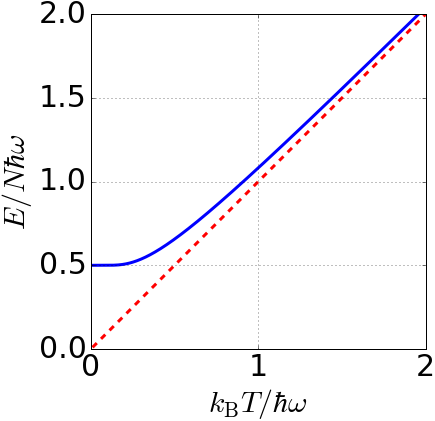
\includegraphics[width=0.15\columnwidth]{Fig/Noszcillator_energia}
\par\end{centering}
\centering{}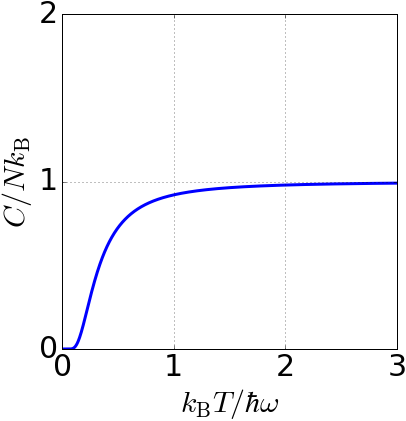
\includegraphics[width=0.15\columnwidth]{Fig/Noszcillator_fajho}\caption{$N$ oszcill�tor energi�ja �s h�kapacit�sa}
\end{wrapfigure}%

A h�m�rs�kletet (\ref{eq:homerseklet})-nek megfelel�en sz�m�tva kapjuk
hogy
\begin{eqnarray}
\frac{1}{T} & = & \left.\frac{\partial S}{\partial E}\right|_{V,N}=\left.\frac{\partial S}{\partial M}\right|_{V,N}\underbrace{\left.\frac{\partial M}{\partial E}\right|_{V,N}}_{1/\hbar\omega}=\frac{k_{\mathrm{B}}}{\hbar\omega}\left[\ln\left(M+N\right)+1-\ln M-1\right]=\frac{k_{\mathrm{B}}}{\hbar\omega}\ln\frac{M+N}{M}\\
 & = & \frac{k_{\mathrm{B}}}{\hbar\omega}\ln\frac{\frac{E}{\hbar\omega}+\frac{N}{2}}{\frac{E}{\hbar\omega}-\frac{N}{2}}=\frac{k_{\mathrm{B}}}{\hbar\omega}\ln\frac{\alpha+\frac{1}{2}}{\alpha-\frac{1}{2}},\quad\alpha=\frac{E}{\hbar\omega N}.
\end{eqnarray}
A h�m�rs�klet teh�t $E/N$ f�ggv�nye azaz, tal�n nem t�l meglep� m�don,
intenz�v mennyis�g! Exponencializ�lva ezt a kifejez�st kapjuk hogy
\begin{equation}
\frac{\alpha+\frac{1}{2}}{\alpha-\frac{1}{2}}=\mathrm{e}^{\frac{\hbar\omega}{k_{\mathrm{B}}T}}=\mathrm{e}^{x},\quad x=\frac{\hbar\omega}{k_{\mathrm{B}}T}.
\end{equation}
Amelyb�l n�mi algebra ut�n az energia a h�m�rs�klet f�gg�s�re kapjuk
hogy
\begin{equation}
\alpha=\left(\frac{1}{2}+\frac{1}{\mathrm{e}^{x}-1}\right)
\end{equation}
\begin{equation}
E=N\hbar\omega\left(\frac{1}{2}+\frac{1}{\mathrm{e}^{\frac{\hbar\omega}{k_{\mathrm{B}}T}}-1}\right).
\end{equation}
Az energia alacsony h�m�rs�kleten j� k�zel�t�ssel 
\begin{equation}
E\approx N\frac{\hbar\omega}{2}.
\end{equation}
Magas h�m�rs�kleten, azaz $x\rightarrow0$ eset�n a k�vetkez� k�zel�t�s
alkalmazhat�: 
\begin{equation}
\frac{E}{N\hbar\omega}=\frac{1}{2}+\left(\frac{1}{\mathrm{e}^{x}-1}\right)\approx\frac{1}{2}+\left(\frac{1}{1+x+\frac{x^{2}}{2}-1}\right)=\frac{1}{2}+\frac{1}{x}\left(\frac{1}{1+\frac{x}{2}}\right)\approx\frac{1}{2}+\frac{1}{x}\left(1-\frac{x}{2}\right)=\frac{1}{x},
\end{equation}
teh�t $k_{\mathrm{B}}T\gg\hbar\omega$ eset�n
\begin{equation}
E\approx Nk_{\mathrm{B}}T.
\end{equation}
A h�kapacit�s ezek ut�n 
\begin{eqnarray}
C & = & \left.\frac{\partial E}{\partial T}\right|_{V}=\frac{\partial E}{\partial x}\frac{\partial x}{\partial T}=-\frac{\hbar\omega}{k_{\mathrm{B}}T^{2}}\frac{\partial E}{\partial x}\\
 & = & -Nk_{\mathrm{B}}\left(\frac{\hbar\omega}{k_{\mathrm{B}}T}\right)^{2}\frac{\partial}{\partial x}\left(\frac{1}{2}+\frac{1}{\mathrm{e}^{x}-1}\right)\nonumber \\
 & = & -Nk_{\mathrm{B}}x^{2}\left(\frac{-1}{\left(\mathrm{e}^{x}-1\right)^{2}}\mathrm{e}^{x}\right)\nonumber \\
 & = & Nk_{\mathrm{B}}\left(\frac{x/2}{\sinh\left(x/2\right)}\right)^{2}\nonumber \\
C & = & Nk_{\mathrm{B}}\left(\frac{\frac{\hbar\omega}{2k_{\mathrm{B}}T}}{\sinh\left(\frac{\hbar\omega}{2k_{\mathrm{B}}T}\right)}\right)^{2}
\end{eqnarray}


\section{Ide�lis g�z}

Vizsg�ljunk meg most az ide�lis g�z eset�t. A Hamilton-f�ggv�ny a
szok�sos

\begin{equation}
H=\sum_{i=1}^{3N}\frac{p_{i}^{2}}{2m}
\end{equation}
alakot �lti. Adott $E$ energia alatt az �llapotok $\Omega_{0}$ sz�m�t
a \href{https://en.wikipedia.org/wiki/Gibbs_paradox}{Gibbs-paradoxon}
figyelembev�tel�vel ($N!$ a nevez�ben) az al�bbiak szerint fejezhetj�k
ki 
\begin{equation}
\Omega_{0}=\int_{H(p,q)<E}\frac{\mathrm{d}^{3N}p\mathrm{d}^{3N}q}{h^{3N}{\color{red}N!}}=\frac{V^{N}}{h^{3N}N!}\int_{\sum_{i=1}^{3N}\frac{p_{i}^{2}}{2m}<E}\mathrm{d}^{3N}p.
\end{equation}
Az impulzus t�rbeli integr�l a (\ref{eq:D-dim-gomb-terfogat-eggyutthat})
seg�ts�g�vel ki�rt�kelhet� mint egy $\sqrt{2mE}$ sugar� $3N$ dimenzi�s
g�mb t�rfogata:
\begin{equation}
\Omega_{0}=\frac{V^{N}}{h^{3N}N!}\frac{\pi^{3N/2}}{\left(\frac{3N}{2}\right)!}\left(\sqrt{2mE}\right)^{3N}=\frac{1}{N!}\frac{1}{\left(\frac{3N}{2}\right)!}\left(\frac{2\pi mEV^{\frac{2}{3}}}{h^{2}}\right)^{\frac{3}{2}N}.
\end{equation}
Az entr�pia meghat�roz�s�hoz $\Omega$ helyett (\ref{eq:entropia-praktice})
szerint termodinamikai hat�resetben $\Omega_{0}$-t is haszn�lhatjuk.
\begin{eqnarray}
S/k_{\mathrm{B}} & = & \ln\Omega_{0}\\
 & = & \frac{3}{2}N\ln\left(\frac{2\pi mEV^{\frac{2}{3}}}{h^{2}}\right)-\ln N!-\ln\left(\frac{3N}{2}\right)!\nonumber \\
\text{Stirling-formula szerint} & \approx & \frac{3}{2}N\ln\left(\frac{2\pi mEV^{\frac{2}{3}}}{h^{2}}\right)-N\ln N+N-\left(\frac{3N}{2}\right)\ln\left(\frac{3N}{2}\right)+\left(\frac{3N}{2}\right)\nonumber \\
 & = & \frac{3}{2}N\ln\left(\frac{2\pi mEV^{\frac{2}{3}}}{h^{2}}\right)-\frac{3}{2}N\ln N^{\frac{2}{3}}+N-\left(\frac{3N}{2}\right)\ln\left(\frac{3N}{2}\right)+\left(\frac{3N}{2}\right)\nonumber \\
 & = & \frac{5}{2}N+\frac{3}{2}N\ln\left(\frac{2\pi mEV^{\frac{2}{3}}}{h^{2}}\frac{1}{N^{\frac{2}{3}}}\frac{2}{3N}\right)\nonumber \\
 & = & \frac{5}{2}N+\frac{3}{2}N\ln\left(\frac{4\pi m}{3h^{2}}\left(\frac{V}{N}\right)^{\frac{2}{3}}\frac{E}{N}\right)\nonumber \\
 & = & N\left[\frac{3}{2}\ln\frac{2}{3}\frac{E}{N}+\ln\frac{V}{N}+\ln\left(\frac{\left(2\pi m\right)^{3/2}}{h^{3}}\mathrm{e}^{5/2}\right)\right]
\end{eqnarray}
Kiindulva a h�m�rs�kletet (\ref{eq:homerseklet}) �s a nyom�st (\ref{eq:nyomas})
defini�l� �sszef�gg�sekb�l megkapjuk az \href{https://hu.wikipedia.org/wiki/Ekvipart\%C3\%ADci\%C3\%B3-t\%C3\%A9tel}{ekvipartici�-t�telb�l}
ismert energia kifejez�st
\begin{equation}
\frac{1}{T}=\left.\frac{\partial S}{\partial E}\right|_{V,N}=\frac{3}{2}Nk_{\mathrm{B}}\frac{1}{E},\Rightarrow E=\frac{3}{2}Nk_{\mathrm{B}}T,\label{eq:idgaz-equipart}
\end{equation}
�s az \href{https://en.wikipedia.org/wiki/Gas_laws}{ide�lis g�z �llapotegyenlet�t}
\begin{equation}
\frac{p}{T}=\left.\frac{\partial S}{\partial V}\right|_{E,N}=\frac{Nk_{\mathrm{B}}}{V},\Rightarrow pV=Nk_{\mathrm{B}}T.
\end{equation}
A k�miai potenci�l (\ref{eq:kemiai-potencial}) alapj�n
\begin{eqnarray}
\mu & = & -T\left.\frac{\partial S}{\partial N}\right|_{E,V}=-k_{\mathrm{B}}T\left[\frac{3}{2}\ln\frac{2}{3}\frac{E}{N}+\ln\frac{V}{N}+\ln\left(\frac{\left(2\pi m\right)^{3/2}}{h^{3}}\mathrm{e}^{5/2}\right)-\frac{3}{2}-1\right],\\
 & = & -k_{\mathrm{B}}T\left[\frac{3}{2}\ln\frac{2}{3}\frac{E}{N}+\ln\frac{V}{N}+\ln\left(\frac{\left(2\pi m\right)^{3/2}}{h^{3}}\right)\right],\\
 & = & -k_{\mathrm{B}}T\left[\ln\frac{V}{N}+\frac{3}{2}\ln\left(\frac{2\pi mk_{\mathrm{B}}T}{h^{2}}\right)\right].
\end{eqnarray}
Ahogy v�rtuk a k�miai potenci�l is intenz�v mennyis�g. 

\shadowbox{\begin{minipage}[t]{0.9\columnwidth}%
\begin{xca}
Hat�rozzuk meg a h�m�rs�klet a nyom�s �s a k�miai potenci�lra vonatkoz�
�sszef�gg�seket a klasszikus relativisztikus ``foton'' g�z eset�re!
Azaz ha egy r�szecsk�re vonatkoz� Hamilton-f�ggv�ny 
\begin{equation}
H=c\left|p\right|.
\end{equation}
\end{xca}
%
\end{minipage}}

\part{�llapot�sszegek kanonikus sokas�gban}

\begin{shaded}%
\textbf{�llapot�sszeg:}

\begin{eqnarray}
\text{Klasszikus rendszer: }Z & = & \frac{1}{h^{N}}\int\left(\mbox{d}p\mbox{d}q\right)^{N}\mathrm{e}^{-\beta H(p,q)}\label{eq:klasszik-Z}\\
 & = & \int_{0}^{\infty}\omega\left(E\right)\mathrm{e}^{-\beta E}\mbox{d}E\\
\text{Kvantumos rendszer: }Z & = & \sum_{n}\mathrm{e}^{-\beta E_{n}}\label{eq:kvanum-Z}
\end{eqnarray}
\begin{equation}
\beta=\frac{1}{k_{\mathrm{B}}T}
\end{equation}

\textbf{Az $n$-edik �llapot bet�lt�s�nek val�sz�n�s�ge:}
\begin{equation}
P_{n}=\frac{\mathrm{e}^{-\beta E_{n}}}{Z}
\end{equation}

\textbf{Szabadenergia:
\begin{equation}
F=-k_{\mathrm{B}}T\ln Z\label{eq:szabad_energia_lnz}
\end{equation}
\begin{equation}
F(T,V,N)=E-TS\label{eq:szabad_energia_legendre}
\end{equation}
\begin{equation}
\mathrm{d}F=-S\mathrm{d}T-p\mathrm{d}V+\mu\mathrm{d}N\label{eq:szabad_energia_diferencialis_alak}
\end{equation}
}

\textbf{Energia (�tlagos):}

\begin{equation}
E=-\frac{\partial}{\partial\beta}\ln Z=-\frac{1}{Z}\frac{\partial Z}{\partial\beta}=\frac{\int_{0}^{\infty}\omega\left(E\right)E\mathrm{e}^{-\beta E}\mbox{d}E}{\int_{0}^{\infty}\omega\left(E\right)\mathrm{e}^{-\beta E}\mbox{d}E}\label{eq:kanonikus-energia}
\end{equation}

\textbf{Nyom�s:}
\begin{equation}
p=-\left.\frac{\partial F}{\partial V}\right|_{T,N}\label{eq:kanonikus-nyomas}
\end{equation}

\textbf{Entr�pia:}
\begin{equation}
S=-\left.\frac{\partial F}{\partial T}\right|_{V,N}\label{eq:kanonikus-entropia-derival}
\end{equation}
\end{shaded}

\section{Mikrokanonikus vs. Kanonikus formalizmus, k�t egyszer� p�lda}

\subsection{Fajh�}

Legyen egy rendszer �llapots�r�s�ge az energia hatv�nyf�ggv�nye, azaz
\begin{equation}
\omega\left(E\right)=A\left(N\right)E^{\alpha N}.
\end{equation}
Sz�m�tsuk ki mikrokanonikus �s kanonikus formalizmusban a fajh�t!

\subsubsection*{Mikrokanonikus}

Kiindulva az entr�pia sz�m�t�s�ra vonatkoz� (\ref{eq:entropia-praktice})
praktikus �sszef�gg�sb�l kapjuk hogy

\begin{equation}
S=k_{\mathrm{B}}\ln\omega\left(E\right)\delta E=k_{\mathrm{B}}\ln A\left(N\right)E^{\alpha N}\delta E=k_{\mathrm{B}}\alpha N\ln E+k_{\mathrm{B}}\ln A\left(N\right)\delta E.
\end{equation}
A h�m�rs�klet (\ref{eq:homerseklet}) alapj�n
\begin{equation}
\frac{1}{T}=\left.\frac{\partial S}{\partial E}\right|_{V,N}=\frac{k_{\mathrm{B}}\alpha N}{E}.
\end{equation}
Az energia illetve a fajh� pedig
\begin{equation}
E=k_{\mathrm{B}}\alpha NT,\rightarrow C=\frac{\partial E}{\partial T}=k_{\mathrm{B}}\alpha N.
\end{equation}


\subsubsection*{Kanonikus}

Az �llapot�sszeget (\ref{eq:klasszik-Z}) alapj�n 

\begin{equation}
Z=\int_{0}^{\infty}\omega\left(E\right)\mathrm{e}^{-\beta E}\mbox{d}E=\int_{0}^{\infty}A\left(N\right)E^{\alpha N}\mathrm{e}^{-\beta E}\mbox{d}E,
\end{equation}
egy v�ltoz� csere v�grehajt�s�val
\begin{equation}
u=\beta E,\quad\mbox{d}E=\frac{\mbox{d}u}{\beta},
\end{equation}
kapjuk hogy
\begin{eqnarray}
Z & = & \int_{0}^{\infty}A\left(N\right)\left(\frac{u}{\beta}\right)^{\alpha N}\mathrm{e}^{-u}\frac{\mbox{d}u}{\beta}=A\left(N\right)\beta^{-(\alpha N+1)}\underbrace{\int_{0}^{\infty}u^{\alpha N}\mathrm{e}^{-u}\mbox{d}u}_{\Gamma\left(\alpha N+1\right)},\\
 & = & A\left(N\right)\beta^{-(\alpha N+1)}\Gamma\left(\alpha N+1\right).
\end{eqnarray}
V�ve ezen kifejez�s logaritmus�t
\begin{equation}
\ln Z=-(\alpha N+1)\ln\beta+\ln A\left(N\right)\Gamma\left(\alpha N+1\right),
\end{equation}
az energia 
\begin{equation}
E=-\frac{\partial}{\partial\beta}\ln Z=\frac{(\alpha N+1)}{\beta}=k_{\mathrm{B}}T(\alpha N+1),
\end{equation}
�s a fajh�
\begin{equation}
C=\frac{\partial E}{\partial T}=k_{\mathrm{B}}(\alpha N+1).
\end{equation}
J�l l�tszik teh�t hogy $N\gg1$ eset�n a k�t formalizmus ugyanazt
adja.

\subsection{Nyom�s}

Legyen egy rendszer �llapots�r�s�ge az energia �s a t�rfogat hatv�nyf�ggv�nye,
azaz
\begin{equation}
\omega\left(E\right)=A\left(\frac{\alpha V}{N}\right)^{N}\left(\frac{E}{N}\right)^{fN}.
\end{equation}
Sz�m�tsuk ki mikrokanonikus �s kanonikus formalizmusban a nyom�st!

\subsubsection*{Mikrokanonikus}

Az el�z� feladathoz hasonl�an az entr�pia (\ref{eq:entropia-praktice})
alapj�n

\begin{equation}
S=k_{\mathrm{B}}\ln\omega\left(E\right)\delta E=k_{\mathrm{B}}N\ln V+k_{\mathrm{B}}\ln A\left(\frac{\alpha}{N}\right)^{N}\left(\frac{E}{N}\right)^{fN}\delta E.
\end{equation}
A nyom�s pedig (\ref{eq:nyomas}) alapj�n
\begin{equation}
\frac{p}{T}=\left.\frac{\partial S}{\partial V}\right|_{E,N}=\frac{k_{\mathrm{B}}N}{V},\rightarrow p=\frac{k_{\mathrm{B}}NT}{V}
\end{equation}


\subsection*{Kanonikus}

Az �llapot�sszeg ism�telten (\ref{eq:klasszik-Z}) szerint
\begin{eqnarray}
Z & = & \int_{0}^{\infty}\omega\left(E\right)\mathrm{e}^{-\beta E}\mbox{d}E=\int_{0}^{\infty}A\left(\frac{\alpha V}{N}\right)^{N}\left(\frac{E}{N}\right)^{fN}\mathrm{e}^{-\beta E}\mbox{d}E\\
 & = & V^{N}\times\left(\mbox{...kutty-kurutty...}\right)
\end{eqnarray}
Melyb�l a szabadenergia az (\ref{eq:szabad_energia_lnz}) �sszef�gg�sb�l
\begin{equation}
F=-k_{\mathrm{B}}T\ln Z=-k_{\mathrm{B}}TN\ln V+\dots
\end{equation}
�s a nyom�s a (\ref{eq:kanonikus-nyomas}) kifejez�sb�l 
\begin{equation}
p=-\left.\frac{\partial F}{\partial V}\right|_{T,N}=\frac{k_{\mathrm{B}}TN}{V}
\end{equation}
ad�dik.

\section{Rot�tor}

\subsection{Klasszikus}

Induljunk ki a (\ref{eq:rotator-hamilton-klasszik}) Hamilton-f�ggv�nyb�l

\begin{equation}
H=\frac{1}{2\Theta}\left(p_{\vartheta}^{2}+\frac{p_{\varphi}^{2}}{\sin^{2}\vartheta}\right).
\end{equation}
Az �llapot�sszeg klasszikus rendszerekre vonatkoz� (\ref{eq:klasszik-Z})
alakj�t felhaszn�lva kapjuk hogy 
\begin{eqnarray}
Z & = & \frac{1}{h^{2}}\int_{0}^{2\pi}\mbox{d}\varphi\int_{0}^{\pi}\mbox{d}\vartheta\underbrace{\int_{-\infty}^{\infty}\mbox{d}p_{\vartheta}\int_{-\infty}^{\infty}\mbox{d}p_{\varphi}\mathrm{e}^{-\frac{\beta}{2\Theta}\left(p_{\vartheta}^{2}+\frac{p_{\varphi}^{2}}{\sin^{2}\vartheta}\right)}}_{\text{2 db Gauss integr�l!!}},\\
 & = & \frac{1}{h^{2}}\underbrace{\int_{0}^{2\pi}\mbox{d}\varphi\int_{0}^{\pi}\mbox{d}\vartheta\sin\vartheta}_{\text{T�rsz�g! \ensuremath{4\pi}}}\sqrt{\frac{2\Theta\pi}{\beta}}\sqrt{\frac{2\Theta\pi}{\beta}},\nonumber \\
 & = & \frac{2\Theta}{\hbar^{2}\beta}.\nonumber 
\end{eqnarray}
Azaz 
\begin{equation}
\ln Z=\ln\frac{2\Theta}{\hbar^{2}}-\ln\beta,
\end{equation}
Melyb�l az energia a szok�sos (\ref{eq:kanonikus-energia}) m�don
\begin{equation}
E=-\frac{\partial}{\partial\beta}\ln Z=\frac{\partial}{\partial\beta}\ln\beta=\frac{1}{\beta}=k_{\mathrm{B}}T.
\end{equation}


\subsection{Kvantumos}

A rot�tor n�v�i (\ref{eq:rotator-kvantum-spektrum}) alapj�n adottak:
\begin{equation}
E_{l}=\frac{\hbar^{2}}{2\Theta}l(l+1).
\end{equation}
Az �llapot�sszeg az egyes n�v�k ismert $(2l+1)$-szeres degener�ci�j�t
figyelembe v�ve
\begin{equation}
Z=\sum_{l=0}^{\infty}\underbrace{\left(2l+1\right)}_{\text{degener�ci� miatt}}\mathrm{e}^{-\beta\frac{\hbar^{2}}{2\Theta}l(l+1)}.
\end{equation}
Alacsony h�m�rs�kleten $\beta\rightarrow\infty$ a legels� nem trivi�lis
j�rul�kot akkor kapjuk ha a k�t legals� energiaszintet figyelembe
vessz�k:
\begin{equation}
Z\underset{T\rightarrow0}{\approx}1+3\mathrm{e}^{-\beta\frac{\hbar^{2}}{2\Theta}2}
\end{equation}
Felhaszn�lva az $\ln$ f�ggv�ny k�zel�t�s�t az $1$k�r�l %
\begin{shaded}%
\begin{equation}
\ln\left(1+x\right)\underset{x\ll1}{\approx}x
\end{equation}
\end{shaded}kapjuk egyszer�en, hogy
\begin{equation}
\ln Z\approx3\mathrm{e}^{-\beta\frac{\hbar^{2}}{\Theta}}.
\end{equation}
Az energia �s a fajh� (\ref{eq:kanonikus-energia}) illetve (\ref{eq:fajho})
alapj�n 
\begin{equation}
E=-\frac{\partial}{\partial\beta}\ln Z=\frac{3\hbar^{2}}{\Theta}\mathrm{e}^{-\beta\frac{\hbar^{2}}{\Theta}},
\end{equation}
\begin{equation}
C=\frac{\partial E}{\partial T}=3\left(\frac{\hbar^{2}}{\Theta}\right)^{2}\frac{1}{k_{\mathrm{B}}T^{2}}\mathrm{e}^{-\frac{\hbar^{2}}{k_{\mathrm{B}}T\Theta}}.
\end{equation}
Magas h�m�rs�kleten egy durva becsl�s, hogy csak azon tagokat vessz�k
melyeknek s�lya legal�bb $1/\mathrm{e}$ �s ezeket �gy vessz�k figyelembe
hogy mindegyiknek ugyanazt a s�lyt adjuk! A feltev�s matematikailag
a legnagyobb $l$-re az al�bbi becsl�st adja 
\begin{equation}
\beta\frac{\hbar^{2}}{2\Theta}l_{max}^{2}=1
\end{equation}
Ezt felhaszn�lva kapjuk hogy 
\begin{equation}
Z=\sum_{l=0}^{l_{max}}\left(2l+1\right)=\left(l_{max}+1\right)^{2}\approx l_{max}^{2}=\frac{2\Theta}{\hbar^{2}\beta}.
\end{equation}


\section{$N$ darab k�t �llapot� rendszer n�mi degener�ci�val}

Sok rendszerben (ahogy l�ttuk a rot�torn�l is) sokszor alacsony h�m�rs�kleten
j� k�zel�t�ssel csak az els� gerjesztett �llapotig tudjuk gerjeszteni
a rendszert: 

\begin{equation}
E_{0}=-\varepsilon,\quad E_{1}=0.
\end{equation}
Az $E_{1}$n�v� $g$-szeresen degener�lt teh�t az �llapot�sszeg 
\begin{equation}
Z=\left(g+\mathrm{e}^{\beta\varepsilon}\right)^{N},
\end{equation}
melyb�l a szabadenergia �s az energia
\begin{equation}
F=-k_{\mathrm{B}}T\ln Z=-k_{\mathrm{B}}TN\ln\left(g+\mathrm{e}^{\beta\varepsilon}\right),
\end{equation}
\begin{equation}
E=-\frac{\partial}{\partial\beta}\ln Z=-N\frac{\partial}{\partial\beta}\ln\left(g+\mathrm{e}^{\beta\varepsilon}\right)=-N\varepsilon\frac{\mathrm{e}^{\beta\varepsilon}}{\left(g+\mathrm{e}^{\beta\varepsilon}\right)},
\end{equation}
Alacsony h�m�rs�kleten kapjuk egyszer�en, hogy
\begin{equation}
T\rightarrow0,\beta\rightarrow\infty,\quad E=-N\varepsilon,
\end{equation}
illetve magas h�m�rs�kleten
\begin{equation}
T\rightarrow\infty,\beta\rightarrow0,\quad E=-N\varepsilon\frac{1}{\left(g+1\right)}.
\end{equation}
Az entr�pi�t (\ref{eq:szabad_energia_legendre}) alapj�n
\begin{equation}
S=\frac{E-F}{T}=k_{\mathrm{B}}N\ln\left(g+\mathrm{e}^{\beta\varepsilon}\right)-\frac{N\varepsilon}{T}\frac{\mathrm{e}^{\beta\varepsilon}}{\left(g+\mathrm{e}^{\beta\varepsilon}\right)}.
\end{equation}
Magas h�m�rs�kleten csak az els� tag j�tszik szerepet,
\begin{equation}
T\rightarrow\infty,\beta\rightarrow0,\quad S=k_{\mathrm{B}}N\ln\left(g+1\right),
\end{equation}
azaz minden �llapot demokratikusan van bet�ltve. Alacsony h�m�rs�kleten
pedig
\begin{eqnarray}
T & \rightarrow & 0,\beta\rightarrow\infty\nonumber \\
S & \approx & k_{\mathrm{B}}N\ln\mathrm{e}^{\beta\varepsilon}\left(g\mathrm{e}^{-\beta\varepsilon}+1\right)-\frac{N\varepsilon}{T}\left(1-g\mathrm{e}^{-\beta\varepsilon}\right),\label{eq:entropia-degeneralt-2szint}\\
 & = & k_{\mathrm{B}}N\left(\beta\varepsilon+g\mathrm{e}^{-\beta\varepsilon}\right)-\frac{N\varepsilon}{T}\left(1-g\mathrm{e}^{-\beta\varepsilon}\right),\nonumber \\
 & = & g\mathrm{e}^{-\frac{\varepsilon}{k_{\mathrm{B}}T}}\left(k_{\mathrm{B}}N+\frac{N\varepsilon}{T}\right).\nonumber 
\end{eqnarray}
\shadowbox{\begin{minipage}[t]{0.9\columnwidth}%
\begin{xca}
Hat�rozzuk meg az el�z� feladatban kisz�m�tott entr�pi�t mikrokanonikus
formalizmusban is! 
\end{xca}
%
\end{minipage}}

Sz�m�tsuk ki a $C$ fajh�t $T=0$ k�rnyezet�ben $F$-en illetve $E$-n
kereszt�l! C�lszer� el�sz�r egy k�zel�t� kifejez�st keresni $\ln Z$-re:
\begin{equation}
\ln Z=N\ln\mathrm{e}^{\beta\varepsilon}\left(1+g\mathrm{e}^{-\beta\varepsilon}\right)\approx Ng\mathrm{e}^{-\beta\varepsilon}+N\beta\varepsilon.
\end{equation}
Ebb�l a szabadenergia
\begin{eqnarray}
F & = & -k_{\mathrm{B}}T\ln Z=-k_{\mathrm{B}}T\left(Ng\mathrm{e}^{-\beta\varepsilon}+N\beta\varepsilon\right),\\
 & = & -\left(k_{\mathrm{B}}TNg\mathrm{e}^{-\frac{\varepsilon}{k_{\mathrm{B}}T}}+N\varepsilon\right).\nonumber 
\end{eqnarray}
Felhaszn�lva (\ref{eq:kanonikus-entropia-derival})-t visszakapjuk
az el�z� (\ref{eq:entropia-degeneralt-2szint}) kifejez�st 
\begin{eqnarray}
S & = & -\frac{\partial F}{\partial T}=k_{\mathrm{B}}Ng\mathrm{e}^{-\frac{\varepsilon}{k_{\mathrm{B}}T}}+k_{\mathrm{B}}TNg\frac{\varepsilon}{k_{\mathrm{B}}T^{2}}\mathrm{e}^{-\frac{\varepsilon}{k_{\mathrm{B}}T}},\\
 & = & k_{\mathrm{B}}Ng\mathrm{e}^{-\frac{\varepsilon}{k_{\mathrm{B}}T}}+Ng\frac{\varepsilon}{T}\mathrm{e}^{-\frac{\varepsilon}{k_{\mathrm{B}}T}}=g\mathrm{e}^{-\frac{\varepsilon}{k_{\mathrm{B}}T}}\left(k_{\mathrm{B}}N+\frac{N\varepsilon}{T}\right).\nonumber 
\end{eqnarray}
A fajh� a l�ncszab�ly haszn�lat�val 
\begin{eqnarray}
C & = & \frac{\partial E}{\partial T}=\underbrace{\frac{\partial E}{\partial S}}_{T}\frac{\partial S}{\partial T}=T\left[g\mathrm{e}^{-\frac{\varepsilon}{k_{\mathrm{B}}T}}\frac{\varepsilon}{k_{\mathrm{B}}T^{2}}\left(k_{\mathrm{B}}N+\frac{N\varepsilon}{T}\right)-g\mathrm{e}^{-\frac{\varepsilon}{k_{\mathrm{B}}T}}\frac{N\varepsilon}{T^{2}}\right],\\
 & = & g\mathrm{e}^{-\frac{\varepsilon}{k_{\mathrm{B}}T}}\left(\frac{\varepsilon}{k_{\mathrm{B}}T}\left(k_{\mathrm{B}}N+\frac{N\varepsilon}{T}\right)-\frac{N\varepsilon}{T}\right)=g\mathrm{e}^{-\frac{\varepsilon}{k_{\mathrm{B}}T}}\left(\left(\frac{\varepsilon N}{T}+N\frac{\varepsilon^{2}}{k_{\mathrm{B}}T^{2}}\right)-\frac{N\varepsilon}{T}\right),\\
 & = & Ngk_{\mathrm{B}}\left(\frac{\varepsilon}{k_{\mathrm{B}}T}\right)^{2}\mathrm{e^{-\frac{\varepsilon}{k_{\mathrm{B}}T}}}.
\end{eqnarray}
Ha az energi�b�l indulunk ki akkor n�mileg r�videbb �ton c�lba �r�nk
\begin{equation}
E=-\frac{\partial}{\partial\beta}\ln Z=Ng\varepsilon\mathrm{e}^{-\beta\varepsilon}-N\varepsilon=N\varepsilon\left(g\mathrm{e}^{-\beta\varepsilon}-1\right)=N\varepsilon\left(g\mathrm{e}^{-\frac{\varepsilon}{k_{\mathrm{B}}T}}-1\right),
\end{equation}
\begin{equation}
C=\frac{\partial E}{\partial T}=N\varepsilon g\mathrm{e}^{-\frac{\varepsilon}{k_{\mathrm{B}}T}}\left(-\frac{\varepsilon}{k_{\mathrm{B}}}\right)\left(-\frac{1}{T^{2}}\right)=Ngk_{\mathrm{B}}\left(\frac{\varepsilon}{k_{\mathrm{B}}T}\right)^{2}\mathrm{e^{-\frac{\varepsilon}{k_{\mathrm{B}}T}}}.
\end{equation}
\shadowbox{\begin{minipage}[t]{0.9\columnwidth}%
\begin{xca}
Egy rendszer fajh�je $C=fk_{\mathrm{B}}$ hat�rozzuk meg a rendszer
�llapots�r�s�g�t!
\end{xca}
%
\end{minipage}}

\newpage{}

\part{Fizikai mennyis�gek eloszl�sai}

\begin{shaded}%
\textbf{V�rhat� �rt�kek:}

\begin{eqnarray}
\text{Klasszikus rendszer: }\left\langle A\right\rangle  & = & \frac{1}{Zh^{N}}\int\left(\mbox{d}p\mbox{d}q\right)^{N}A(p,q)\mathrm{e}^{-\beta H(p,q)}\label{eq:klasszik-varhato-ertek}\\
\text{Kvantumos rendszer: }\left\langle A\right\rangle  & = & \frac{1}{Z}\sum_{n}\left\langle n\left|\hat{A}\right|n\right\rangle \mathrm{e}^{-\beta E_{n}}\label{eq:kvanum-varhato-ertek}
\end{eqnarray}

\textbf{Deriv�ltak v�rhat� �rt�ke (\href{https://en.wikipedia.org/wiki/Hellmann\%E2\%80\%93Feynman_theorem}{Hellmann-Feynman t�tel}):}

\begin{equation}
\left\langle \frac{\partial}{\partial\lambda}H(\lambda)\right\rangle =\frac{\partial}{\partial\lambda}F(\lambda)\label{eq:hellmann-feynman-tetel}
\end{equation}

\textbf{Ekvipartici� t�tel}

Ha

\textbf{
\begin{equation}
H=\lambda_{1}x_{1}^{2}+g(x_{2},x_{3},\dots),
\end{equation}
}

akkor 

\selectlanguage{english}%
\inputencoding{latin9}\begin{equation}
\left\langle \lambda_{1}x_{1}^{2}\right\rangle =\frac{1}{2}k_{\mathrm{B}}T,\label{eq:ekviparticio-tetel}
\end{equation}

\selectlanguage{magyar}%
\inputencoding{latin2}%
�ltal�nosabban
\begin{equation}
\left\langle x_{i}\frac{\partial H}{\partial x_{j}}\right\rangle =k_{\mathrm{B}}T\delta_{ij}\label{eq:altalanos-ekviparticio-tetel}
\end{equation}
\end{shaded}

\section{K�t�llapot� rendszerek energia eloszl�sai}

\begin{equation}
Z_{1}=\mathrm{e}^{\beta\varepsilon}+\mathrm{e}^{-\beta\varepsilon}=2\cosh\beta\varepsilon
\end{equation}
\begin{equation}
Z=Z_{1}^{N}=\left(2\cosh\beta\varepsilon\right)^{N},\rightarrow\ln Z=N\ln2\cosh\beta\varepsilon\label{eq:2all-kanonikus-Z}
\end{equation}
\begin{eqnarray}
N_{+} & = & \frac{N+M}{2}=\frac{N}{2}+\frac{E}{2\varepsilon}\\
E & = & \varepsilon\left(2N_{+}-N\right)\label{eq:2allapot-kanonikus-evs-nplus}
\end{eqnarray}
\begin{equation}
\left\langle E\right\rangle =-\partial_{\beta}\ln Z=-N\varepsilon\frac{2\sinh\beta\varepsilon}{2\cosh\beta\varepsilon}=-N\varepsilon\tanh\beta\varepsilon
\end{equation}
\begin{equation}
\left\langle N_{+}\right\rangle =\frac{N}{2}\left[1-\tanh\beta\varepsilon\right]
\end{equation}
Mi a val�sz�n�s�ge hogy $n$ darab r�szecske a $+\varepsilon$ energi�j�
�llapotban van. 
\begin{equation}
P\left(N_{+}=n\right)=\frac{\left(\begin{array}{c}
N\\
n
\end{array}\right)\mathrm{e}^{-\beta E(n)}}{Z}=\frac{\left(\begin{array}{c}
N\\
n
\end{array}\right)\mathrm{e}^{-\beta\varepsilon\left(2n-N\right)}}{Z}
\end{equation}
A legval�sz�n�bb �llapotban 
\begin{equation}
\partial_{n}\ln P=0
\end{equation}
Termodinamikai hat�resetben kihaszn�lva a (\ref{eq:stirling-log})
Stirling-formul�t 
\begin{equation}
\ln\frac{N!}{n!\left(N-n\right)!}\mathrm{e}^{-\beta E(n)}\approx-\beta\varepsilon\left(2n-N\right)+N\ln N-n\ln n-\left(N-n\right)\ln\left(N-n\right)
\end{equation}
\begin{eqnarray}
\partial_{n}\ln P & = & -2\beta\varepsilon-\ln n-1+\ln\left(N-n\right)+1\\
 & = & -2\beta\varepsilon+\ln\frac{N-n}{n}
\end{eqnarray}
kapjuk teh�t hogy a legval�sz�n�bb �llapotban a pozit�v energi�s r�szecsk�k
sz�ma
\begin{equation}
n=N\frac{1}{\mathrm{e}^{2\beta\varepsilon}+1}.
\end{equation}
Vizsg�ljuk meg ennek az eloszl�snak a sz�r�s�t, azaz hat�rozzuk meg
a k�vetkez� mennyis�get
\begin{equation}
\left\langle N_{+}^{2}\right\rangle -\left\langle N_{+}\right\rangle ^{2}=?
\end{equation}
Ez a mennyis�g (\ref{eq:2allapot-kanonikus-evs-nplus}) alapj�n az
energia �s az energia n�gyzet v�rhat��rt�kkel fejezhet� ki. Az energia
v�rhat��rt�k�nek n�gyzete 
\begin{eqnarray}
\left\langle E\right\rangle  & = & 2\varepsilon\left\langle N_{+}\right\rangle -N\varepsilon,\nonumber \\
\left\langle E\right\rangle ^{2} & = & 4\varepsilon^{2}\left\langle N_{+}\right\rangle ^{2}+N^{2}\varepsilon^{2}-4\varepsilon^{2}\left\langle N_{+}\right\rangle N,
\end{eqnarray}
illetve az energia n�gyzet�nek v�rhat� �rt�ke
\begin{eqnarray}
\left\langle E^{2}\right\rangle  & = & \left\langle \left(2\varepsilon N_{+}-N\varepsilon\right)^{2}\right\rangle ,\\
 & = & \left\langle 4\varepsilon^{2}N_{+}^{2}+N^{2}\varepsilon^{2}-4\varepsilon^{2}NN_{+}\right\rangle ,\nonumber \\
 & = & 4\varepsilon^{2}\left\langle N_{+}^{2}\right\rangle +N^{2}\varepsilon^{2}-4\varepsilon^{2}\left\langle N_{+}\right\rangle N,\nonumber 
\end{eqnarray}
amib�l 
\begin{equation}
\frac{\left\langle E^{2}\right\rangle -\left\langle E\right\rangle ^{2}}{4\varepsilon^{2}}=\left\langle N_{+}^{2}\right\rangle -\left\langle N_{+}\right\rangle ^{2}.
\end{equation}
Az energia tetsz�leges hatv�ny�nak v�rhat��rt�k�t k�nny� szerrel meghat�rozhatjuk
az �llapot�sszeg $\beta$ szerinti dervi�ljaib�l, hiszen
\begin{equation}
\partial_{\beta}^{p}Z=\sum_{j}\left(-E_{j}\right)^{p}\mathrm{e}^{\beta E_{j}}
\end{equation}
teh�t 
\begin{equation}
\left\langle E^{p}\right\rangle =\frac{\left(-1\right)^{p}}{Z}\partial_{\beta}^{p}Z.
\end{equation}
A sz�munkra �rdekes sz�r�s
\begin{equation}
\left\langle E^{2}\right\rangle -\left\langle E\right\rangle ^{2}=\frac{1}{Z}\partial_{\beta}^{2}Z-\left(\partial_{\beta}\ln Z\right)^{2}.
\end{equation}
Felhaszn�lva az �llapot�sszeg (\ref{eq:2all-kanonikus-Z}) kifejez�s�t
a konkr�t probl�m�nkra a relev�ns deriv�ltak:
\begin{eqnarray}
\partial_{\beta}\left(2\cosh\beta\varepsilon\right)^{N} & = & 2N\varepsilon\left(2\cosh\beta\varepsilon\right)^{N-1}\sinh\beta\varepsilon\\
\partial_{\beta}^{2}\left(2\cosh\beta\varepsilon\right)^{N} & = & 2N\varepsilon\left[2\varepsilon\left(N-1\right)\left(2\cosh\beta\varepsilon\right)^{N-2}\sinh^{2}\beta\varepsilon+2^{N-1}\varepsilon\left(\cosh\beta\varepsilon\right)^{N}\right]\\
 & = & \varepsilon^{2}N(N-1)2^{N}\sinh^{2}\beta\varepsilon\cosh^{N-2}\beta\varepsilon+N2^{N}\varepsilon^{2}\left(\cosh\beta\varepsilon\right)^{N}\nonumber 
\end{eqnarray}
Az energia n�gyzet v�rhat� �rt�ke teh�t
\begin{equation}
\left\langle E^{2}\right\rangle =\varepsilon^{2}N(N-1)\tanh^{2}\beta\varepsilon+N\varepsilon^{2}.
\end{equation}
Az energia sz�r�sa
\begin{eqnarray}
\left\langle E^{2}\right\rangle -\left\langle E\right\rangle ^{2} & = & \varepsilon^{2}N(N-1)\tanh^{2}\beta\varepsilon+N\varepsilon^{2}-N^{2}\varepsilon^{2}\tanh^{2}\beta\varepsilon\\
 & = & \varepsilon^{2}N\left(1-\tanh^{2}\beta\varepsilon\right)=\frac{\varepsilon^{2}N}{\cosh^{2}\beta\varepsilon}.\nonumber 
\end{eqnarray}
A bet�lt�si sz�mok keresett sz�r�sa teh�t
\begin{equation}
\left\langle N_{+}^{2}\right\rangle -\left\langle N_{+}\right\rangle ^{2}=\frac{N}{4\cosh^{2}\beta\varepsilon}.
\end{equation}


\section{Rot�tor elektromos t�rben\label{sec:rotator-e-terben}}

\begin{eqnarray}
H & = & E_{kin}+E_{pot}=\frac{1}{2\Theta}\left[p_{\vartheta}^{2}+\frac{p_{\varphi}^{2}}{\sin^{2}\vartheta}\right]-\vec{\mathcal{E}}\cdot\vec{d}\\
 & = & \frac{1}{2\Theta}\left[p_{\vartheta}^{2}+\frac{p_{\varphi}^{2}}{\sin^{2}\vartheta}\right]-\mathcal{E}d\cos\vartheta\nonumber 
\end{eqnarray}
�llapot�sszeg
\begin{eqnarray}
Z & = & \frac{1}{h^{2}}\int_{0}^{2\pi}\mbox{d}\varphi\int_{0}^{\pi}\mbox{d}\vartheta\int_{-\infty}^{\infty}\mbox{d}p_{\vartheta}\int_{-\infty}^{\infty}\mbox{d}p_{\varphi}\mathrm{e}^{-\frac{\beta}{2\Theta}\left(p_{\vartheta}^{2}+\frac{p_{\varphi}^{2}}{\sin^{2}\vartheta}\right)}\mathrm{e}^{\beta\mathcal{E}d\cos\vartheta},\\
 & = & \frac{1}{h^{2}}\int_{0}^{2\pi}\mbox{d}\varphi\int_{0}^{\pi}\mbox{d}\vartheta\mathrm{e}^{\beta\mathcal{E}d\cos\vartheta}\sqrt{\frac{2\Theta\pi}{\beta}}\sqrt{\frac{2\Theta\pi}{\beta}}\sin\vartheta\nonumber \\
 & = & \frac{1}{h^{2}}\frac{2\pi\Theta2\pi}{\beta}\int_{0}^{\pi}\mbox{d}\vartheta\mathrm{e}^{\beta\mathcal{E}d\cos\vartheta}\sin\vartheta,\:\left(\text{v�ltoz�csere:}\,x=\cos\vartheta,\frac{\mathrm{d}x}{\mathrm{d}\vartheta}=-\sin\vartheta\right)\nonumber \\
 & = & \frac{\Theta}{\hbar^{2}\beta}\int_{-1}^{1}\mbox{d}x\mathrm{e}^{\beta\mathcal{E}dx}=\frac{\Theta}{\hbar^{2}\beta}\frac{\mathrm{e}^{\beta\mathcal{E}d}-\mathrm{e}^{-\beta\mathcal{E}d}}{\beta\mathcal{E}d}=\frac{2\Theta\sinh\beta\mathcal{E}d}{\hbar^{2}\beta^{2}d\mathcal{E}}\nonumber 
\end{eqnarray}
Egy $A(\vartheta,\varphi)$ mennyis�g v�rhat� �rt�ke (\ref{eq:klasszik-varhato-ertek})-nek
megfelel�en
\begin{equation}
\int\mbox{d}\varphi\mbox{d}\vartheta A(\vartheta,\varphi)\int\frac{\mbox{d}p_{\vartheta}\mbox{d}p_{\varphi}}{h^{2}}\frac{\mathrm{e}^{-\beta H}}{Z}=\int\mbox{d}\varphi\mbox{d}\vartheta A(\vartheta,\varphi)P(\vartheta,\varphi)
\end{equation}
Ahol bevezett�k a $P(\vartheta,\varphi)$ val�sz�n�s�gi s�r�s�get.
\begin{eqnarray}
P(\vartheta,\varphi) & = & \frac{1}{h^{2}Z}\int_{-\infty}^{\infty}\mbox{d}p_{\vartheta}\mbox{d}p_{\varphi}\mathrm{e}^{-\beta H}\\
 & = & \frac{\mathrm{e}^{\beta\mathcal{E}d\cos\vartheta}}{h^{2}Z}\int_{-\infty}^{\infty}\mbox{d}p_{\vartheta}\mbox{d}p_{\varphi}\mathrm{e}^{-\frac{\beta}{2\Theta}\left(p_{\vartheta}^{2}+\frac{p_{\varphi}^{2}}{\sin^{2}\vartheta}\right)}\nonumber \\
 & = & \frac{\mathrm{e}^{\beta\mathcal{E}d\cos\vartheta}}{h^{2}Z}\frac{2\Theta\pi}{\beta}\sin\vartheta\nonumber \\
 & = & \frac{\mathrm{e}^{\beta\mathcal{E}d\cos\vartheta}\frac{2\Theta\pi}{\beta}\sin\vartheta}{h^{2}\frac{2\Theta\sinh\beta\mathcal{E}d}{\hbar^{2}\beta^{2}d\mathcal{E}}}\nonumber \\
 & = & \frac{1}{4\pi}\frac{\beta d\mathcal{E}}{\sinh\beta\mathcal{E}d}\mathrm{e}^{\beta\mathcal{E}d\cos\vartheta}\sin\vartheta\nonumber 
\end{eqnarray}
Vegy�k �szre hogy $\mathcal{E}=0$ eset�n illetve magas h�m�rs�kleten
amikor $\beta=0$ 
\begin{equation}
P(\vartheta,\varphi)\mbox{d}\varphi\mbox{d}\vartheta=\frac{\sin\vartheta\mbox{d}\varphi\mbox{d}\vartheta}{4\pi}=\frac{\mbox{d}\Omega}{4\pi}
\end{equation}
azaz ahogy v�rjuk ha a rendszerben nincs kit�ntetett ir�ny, vagy a
termikus fluktu�ci�k mindent ki�tlagolnak akkor a sz�g szerinti eloszl�s
egyenletes!

Ha a rendszer tulajdons�gai f�ggetlenek $\varphi$-t�l akkor �rdemes
bevezetni a 
\begin{equation}
\bar{P}\left(\vartheta\right)=\int_{0}^{2\pi}P(\vartheta,\varphi)\mbox{d}\varphi=\frac{1}{2}\frac{\beta d\mathcal{E}}{\sinh\beta\mathcal{E}d}\mathrm{e}^{\beta\mathcal{E}d\cos\vartheta}\sin\vartheta\label{eq:ERrotator-eloszlas-theta}
\end{equation}
�tlagolt eloszl�sf�ggv�nyt. 

Hat�rozzuk meg az energia v�rhat� �rt�k�t!
\begin{eqnarray}
E & = & -\partial_{\beta}\ln Z=-\partial_{\beta}\left[\ln\frac{2\Theta}{\hbar^{2}d\mathcal{E}}+\ln\left(\sinh\beta\mathcal{E}d\right)-2\ln\beta\right]\\
 & = & \frac{2}{\beta}-\mathcal{E}d\frac{\cosh\beta\mathcal{E}d}{\sinh\beta\mathcal{E}d}=\frac{1}{\beta}-\mathcal{E}d\left[\coth\beta\mathcal{E}d-\frac{1}{\beta\mathcal{E}d}\right]\nonumber \\
 & = & k_{\mathrm{B}}T-\mathcal{E}d\mathcal{L}\left(\beta\mathcal{E}d\right)\nonumber 
\end{eqnarray}
\begin{wrapfigure}{o}{0.3\columnwidth}%
\begin{centering}
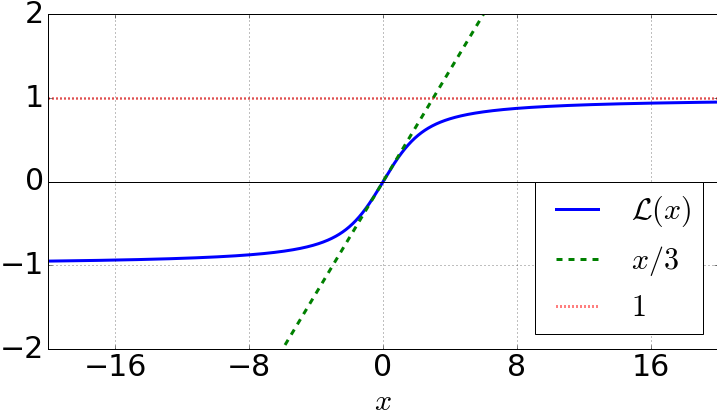
\includegraphics[width=0.3\textwidth]{Fig/Langevin}
\par\end{centering}
\caption{A Langevin-f�ggv�ny\label{fig:Langevin-fuggveny}}
\end{wrapfigure}%
\parbox[t]{0.67\columnwidth}{%
\begin{shaded}%
ahol bevezett�k a \href{https://en.wikipedia.org/wiki/Brillouin_and_Langevin_functions}{Langevin-f�ggv�nyt}:
\begin{equation}
\mathcal{L}\left(x\right)=\coth x-\frac{1}{x}
\end{equation}
\end{shaded}%
}

Hat�rozzuk meg a rendszer dip�lmomentum�nak v�rhat� �rt�k�t. A meghat�rozand�
v�rhat��rt�k 
\begin{equation}
\left\langle d_{\mathcal{E}}\right\rangle =\left\langle d\cos\vartheta\right\rangle 
\end{equation}
Induljunk ki a Hellmann\textendash Feynman-t�telb�l (\ref{eq:hellmann-feynman-tetel}):
\begin{eqnarray}
\left\langle d\cos\vartheta\right\rangle  & = & -\left\langle \partial_{\mathcal{E}}H\right\rangle =\frac{1}{\beta}\partial_{\mathcal{E}}\ln Z\\
 & = & \frac{1}{\beta}\partial_{\mathcal{E}}\left[\ln\frac{2\Theta}{\hbar^{2}\beta^{2}d}+\ln\left(\sinh\beta\mathcal{E}d\right)-\ln\mathcal{E}\right]\nonumber \\
 & = & \frac{1}{\beta}\left[\beta d\frac{\cosh\beta\mathcal{E}d}{\sinh\beta\mathcal{E}d}-\frac{1}{\mathcal{E}}\right]\nonumber \\
 & = & d\left[\frac{\cosh\beta\mathcal{E}d}{\sinh\beta\mathcal{E}d}-\frac{1}{\beta\mathcal{E}d}\right]=d\mathcal{L}\left(\beta\mathcal{E}d\right)\label{eq:ratator-eter-dipolmomentum}
\end{eqnarray}
Vegy�k �szre hogy ugyan erre a kifejez�sre jutottunk volna ha a v�rhat�
�rt�kek egyszer� defin�ci�j�t haszn�ltuk volna: 
\begin{equation}
\left\langle d\cos\vartheta\right\rangle =\frac{\int_{0}^{\pi}\mathrm{e}^{\beta\mathcal{E}d\cos\vartheta}d\cos\vartheta\sin\vartheta\mathrm{d}\vartheta}{\int_{0}^{\pi}\mathrm{e}^{\beta\mathcal{E}d\cos\vartheta}\sin\vartheta\mathrm{d}\vartheta}=d\frac{\int_{-1}^{1}\mathrm{e}^{\beta\mathcal{E}dx}x\mathrm{d}x}{\int_{-1}^{1}\mathrm{e}^{\beta\mathcal{E}dx}\mathrm{d}x}=\frac{1}{\beta}\partial_{\mathcal{E}}\ln Z.
\end{equation}


\section{F�ggetlen kvantumos m�gneses momentum k�ls� m�gneses t�rben}

\begin{equation}
\hat{H}=-\vec{M}\cdot\vec{B}=-\mu_{B}\hat{\vec{S}}\cdot\vec{B}=-\mu_{B}\hat{S_{z}}B
\end{equation}
$\hat{S_{z}}$ saj�t�rt�kei : $-j,-j+1,\dots j$ ahol a $j$ lehet
eg�sz vagy f�leg�sz sz�m. Az �llapot�sszeg 
\begin{equation}
Z=\sum_{m=-j}^{j}\mathrm{e}^{\beta\mu_{B}mB}
\end{equation}
Vegy�k �szre hogy ez egy \href{https://hu.wikipedia.org/wiki/M\%C3\%A9rtani_sorozat}{m�rtani sorozat}
es� $(2j+1)$ tagj�nak �sszege 
\begin{eqnarray}
Z & = & \mathrm{e}^{-\beta\mu_{B}Bj}\frac{\mathrm{e}^{\beta\mu_{B}B\left(2j+1\right)}-1}{\mathrm{e}^{\beta\mu_{B}B}-1},\\
 & = & \frac{\mathrm{e}^{\beta\mu_{B}B(j+1/2)}-\mathrm{e}^{-\beta\mu_{B}B(j+1/2)}}{\mathrm{e}^{\beta\mu_{B}B/2}-\mathrm{e}^{-\beta\mu_{B}B/2}},\nonumber \\
 & = & \frac{\sinh\left(\beta\mu_{B}B(j+1/2)\right)}{\sinh\left(\beta\mu_{B}B/2\right)}\nonumber 
\end{eqnarray}
Az �llapot�sszeg teh�t $\beta B$ mennyis�g f�ggv�nye. Azaz a rendszerben
jelenlev� k�t meghat�roz� energiask�la a term�lis energia �s a m�gneses
energia h�nyadosa a relev�ns param�ter. A rendszer energi�ja (\ref{eq:kanonikus-energia})
szerint
\begin{eqnarray}
E & = & -\partial_{\beta}\ln Z=-\partial_{\beta}\left[\ln\sinh\left(\beta\mu_{B}B(j+1/2)\right)-\ln\sinh\left(\beta\mu_{B}B/2\right)\right],\\
 & = & -\left[\mu_{B}B(j+1/2)\frac{\cosh\left(\beta\mu_{B}B(j+1/2)\right)}{\sinh\left(\beta\mu_{B}B(j+1/2)\right)}-\mu_{B}B/2\frac{\cosh\left(\beta\mu_{B}B/2\right)}{\sinh\left(\beta\mu_{B}B/2\right)}\right],\nonumber \\
 & = & \mu_{B}B/2\coth\left(\beta\mu_{B}B/2\right)-\mu_{B}B(j+1/2)\coth\left(\beta\mu_{B}B(j+1/2)\right).\nonumber 
\end{eqnarray}
A szabadenergia
\begin{equation}
F=-k_{\mathrm{B}}T\ln Z,
\end{equation}
melyb�l a Hellmann\textendash Feynman-t�tel (\ref{eq:hellmann-feynman-tetel})
seg�ts�g�vel megkapjuk a m�gnesezetts�get 
\begin{equation}
M=-\partial_{B}F=\frac{1}{\beta}\partial_{B}\ln Z\underset{Z=f(\beta B)}{=}-\frac{E}{B},
\end{equation}
\begin{eqnarray}
M & = & \mu_{B}(j+1/2)\coth\left(\beta\mu_{B}B(j+1/2)\right)-\mu_{B}/2\coth\left(\beta\mu_{B}B/2\right)\\
 & = & \mu_{B}j\mathcal{B}_{j}(x),\quad x=\mu_{B}\beta Bj.\nonumber 
\end{eqnarray}

\begin{wrapfigure}{o}{0.3\columnwidth}%
\begin{centering}
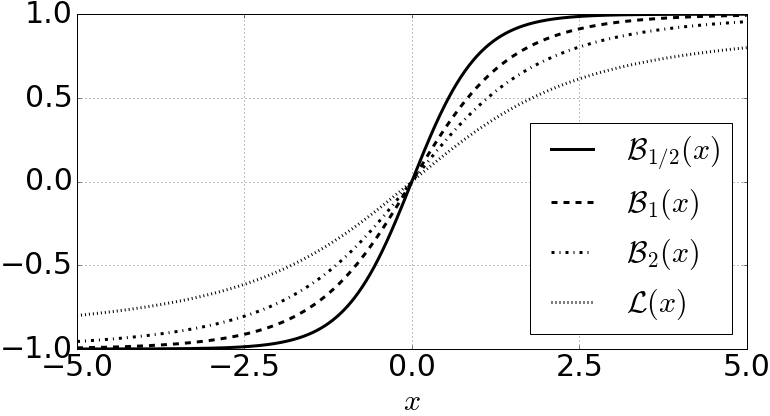
\includegraphics[width=0.3\textwidth]{Fig/Brillouin}
\par\end{centering}
\caption{A Brillouin-f�ggv�ny k�l�nb�z� $j$-kre illetve a Langevin-f�ggv�ny
\label{fig:Brillouin-fuggveny}}
\end{wrapfigure}%

\parbox[t]{0.65\columnwidth}{%
\begin{shaded}%
Ahol bevezett�k a $\mathcal{B}{}_{j}(x)$ \href{https://en.wikipedia.org/wiki/Brillouin_and_Langevin_functions}{Brillouin-f�ggv�nyt}
\begin{equation}
\mathcal{B}_{j}(x)=\frac{2j+1}{2j}\coth\left(\frac{2j+1}{2j}x\right)-\frac{1}{2j}\coth\left(\frac{x}{2j}\right)
\end{equation}
\end{shaded}%
}

Vizsg�ljuk meg a fenn kapott eredm�nyek viselked�s�t nagy m�gneses
t�r illetve alacsony h�m�rs�klet mellett azaz ha a Brillouin-f�ggv�ny
argumentuma nagy, vagyis 
\begin{eqnarray}
x & = & \mu_{B}\beta Bj\gg1.
\end{eqnarray}

A $\coth(x)$ f�ggv�ny ezen a tartom�nyon j� k�zel�t�ssel $\coth\left(x\right)\approx1.$
A m�gnesezetts�g teh�t
\begin{equation}
M\approx\mu_{B}\left[\frac{2j+1}{2}-\frac{1}{2}\right]=\mu_{B}j.
\end{equation}

Azaz ahogy v�rjuk csak a legkisebb energi�j� �lapot ad j�rul�kot.

Az ellent�tes hat�resetben azaz nagy h�m�rs�klet vagy kicsi m�gneses
t�r eset�n az vagyis 
\begin{eqnarray}
x & = & \mu_{B}\beta Bj\ll1
\end{eqnarray}
\begin{wrapfigure}{o}{0.2\columnwidth}%
\begin{centering}
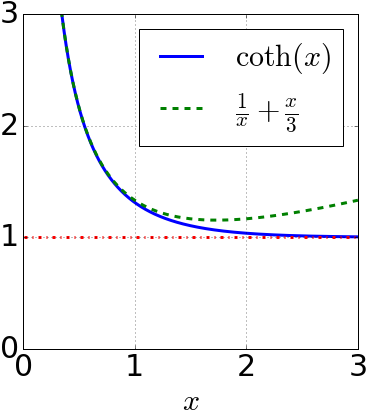
\includegraphics[width=0.15\textwidth]{Fig/coth}
\par\end{centering}
\caption{A $\coth(x)$ f�ggv�ny �s k�zel�t�sei.}
\end{wrapfigure}%

Ekkor

\begin{equation}
\coth\left(x\right)\approx\frac{1}{x}+\frac{x}{3},
\end{equation}
a Brillouin-f�ggv�ny pedig

\begin{eqnarray}
\mathcal{B}_{j}(x) & \underset{x\rightarrow0}{\approx} & \frac{2j+1}{2j}\left(\frac{2j}{\left(2j+1\right)x}+\frac{1}{3}\times\frac{2j+1}{2j}x\right)-\frac{1}{2j}\left(\frac{2j}{x}+\frac{1}{3}\frac{x}{2j}\right),\\
 & = & \frac{1}{x}+\frac{x}{3}\left(\frac{2j+1}{2j}\right)^{2}-\frac{1}{x}-\frac{x}{3}\frac{1}{\left(2j\right)^{2}},\\
 & = & \frac{x}{3}\frac{4j^{2}+4j}{\left(2j\right)^{2}}=\frac{x}{3}\frac{j+1}{j}.
\end{eqnarray}
A m�gnesezetts�g teh�t
\begin{equation}
M\approx\mu_{B}^{2}\frac{j\left(j+1\right)}{3k_{\mathrm{B}}T}B.
\end{equation}
Magas h�m�rs�kleten teh�t a \href{https://en.wikipedia.org/wiki/Curie\%E2\%80\%93Weiss_law}{Curie-t�rv�nynek}
megfelel� viselked�st kapunk
\begin{equation}
\chi=\partial_{B}M=\mu_{B}^{2}\frac{j\left(j+1\right)}{3k_{\mathrm{B}}T}.
\end{equation}

Vizsg�ljuk meg a nagy impulzusmomentum $j\gg1$ hat�resetet, ez a
klasszikus hat�reset. Vegy�k �szre hogy ekkor a Brillouin-f�ggv�ny
a Langevin-f�ggv�nyre egyszer�s�dik 
\begin{equation}
\mathcal{B}_{j}(x)\underset{j\gg1}{\approx}\coth\left(x\right)-\frac{1}{2j}\coth\left(\frac{x}{2j}\right)\approx\coth\left(x\right)-\frac{1}{x}=\mathcal{L}(x),
\end{equation}
a m�gnesezetts�g teh�t
\begin{equation}
M=\mu_{B}j\mathcal{L}(\mu_{B}\beta Bj).
\end{equation}
�rdemes �sszevetni ezt az eredm�nyt a klasszikus rot�tor vizsg�lata
sor�n sz�molt dip�l momentummal (\ref{eq:ratator-eter-dipolmomentum}),
ahol szint�n hasonl� viselked�st kaptunk.

V�g�l foglaljuk �ssze a kapott eredm�nyeket feles spin azaz $j=1/2$
eset�re:
\begin{equation}
Z=2\cosh\left(\frac{\beta\mu_{B}B}{2}\right)
\end{equation}
\begin{equation}
E=-\frac{\mu_{B}B}{2}\tanh\left(\frac{\beta\mu_{B}B}{2}\right)
\end{equation}

\begin{equation}
M=\frac{\mu_{B}}{2}\tanh\left(\frac{\beta\mu_{B}B}{2}\right)
\end{equation}


\section{2D oszcill�tor}

\begin{equation}
H=\frac{p_{x}^{2}+p_{y}^{2}}{2m}+\frac{1}{2}m\omega^{2}\left(x^{2}+y^{2}\right)=\frac{\vec{p}\cdot\vec{p}}{2m}+\frac{1}{2}m\omega^{2}\vec{r}\cdot\vec{r}
\end{equation}
Az �llapot�sszeg a klasszikus rendszerekre vonatkoz� (\ref{eq:klasszik-Z})
kifejez�sb�l
\begin{equation}
Z=\frac{1}{h^{2}}\int_{-\infty}^{\infty}\mathrm{d}\vec{p}\mathrm{d}\vec{r}\mathrm{e}^{-\beta\left[\frac{p^{2}}{2m}+\frac{1}{2}m\omega^{2}r^{2}\right]}=\frac{1}{h^{2}}\frac{2\pi m}{\beta}\frac{2\pi}{\beta m\omega^{2}}=\frac{1}{\left(\hbar\beta\omega\right)^{2}}.
\end{equation}
Mennyi a kit�r�s n�gyzet v�rhat� �rt�ke ?
\begin{equation}
\left\langle r^{2}\right\rangle =\frac{1}{Zh^{2}}\int_{-\infty}^{\infty}r^{2}\mathrm{d}\vec{p}\mathrm{d}\vec{r}\mathrm{e}^{-\beta\left[\frac{p^{2}}{2m}+\frac{1}{2}m\omega^{2}r^{2}\right]}
\end{equation}
Vegy�k �szre hogy
\begin{equation}
\partial_{\omega^{2}}Z=\frac{1}{h^{2}}\int_{-\infty}^{\infty}\left(-\frac{1}{2}\beta mr^{2}\right)\mathrm{d}\vec{p}\mathrm{d}\vec{r}\mathrm{e}^{-\beta\left[\frac{p^{2}}{2m}+\frac{1}{2}m\omega^{2}r^{2}\right]}
\end{equation}
teh�t 
\begin{equation}
-\frac{2}{m\beta}\frac{1}{Z}\partial_{\omega^{2}}Z=-\frac{2}{m\beta}\partial_{\omega^{2}}\ln Z=\left\langle r^{2}\right\rangle 
\end{equation}
azaz 
\begin{equation}
\left\langle r^{2}\right\rangle =\frac{2}{m\beta}\partial_{\omega^{2}}\ln\left(\hbar\beta\omega\right)^{2}=\frac{2}{m\beta\omega^{2}}
\end{equation}
�trendezve 
\begin{equation}
\frac{1}{2}m\omega^{2}\left\langle r^{2}\right\rangle =\left\langle E_{pot}\right\rangle =k_{\mathrm{B}}T
\end{equation}
az ekvipartici� t�tel szellem�nek megfelel�en.

Hasonl� eredm�nyre jutunk ha a Hellmann-Feynman t�telt (\ref{eq:hellmann-feynman-tetel})
alkalmazzuk:
\begin{equation}
\partial_{\omega^{2}}H=\frac{1}{2}mr^{2}
\end{equation}
\begin{equation}
\left\langle \partial_{\omega^{2}}H\right\rangle =\frac{1}{2}m\left\langle r^{2}\right\rangle =-\frac{1}{\beta}\partial_{\omega^{2}}\ln Z
\end{equation}


\section{S�kinga}

A s�kinga Lagrange f�ggv�nye, 

\begin{equation}
L=\frac{1}{2}ml^{2}\dot{\varphi}^{2}+mgl\cos\varphi-mgl.
\end{equation}
\begin{wrapfigure}{o}{0.2\columnwidth}%
\begin{centering}
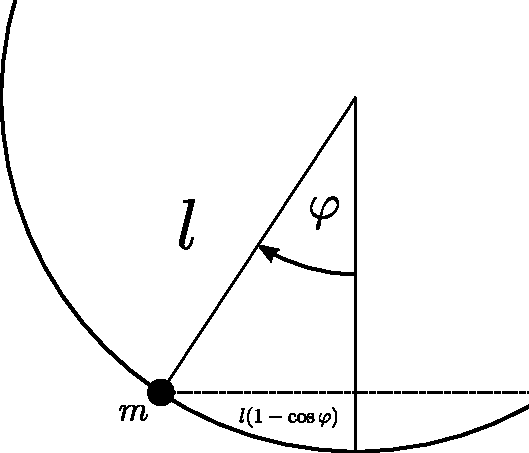
\includegraphics[width=0.2\textwidth]{Fig/sikinga}
\par\end{centering}
\caption{S�kinga}
\end{wrapfigure}%
A $\varphi$-koordin�t�hoz konjug�lt kanonikus impulzus teh�t
\begin{equation}
p_{\varphi}=\frac{\partial L}{\partial\dot{\varphi}}=ml^{2}\dot{\varphi}.
\end{equation}
A Hamilton-f�ggv�ny a k�vetkez� alakot �lti 
\begin{equation}
H=\frac{p_{\varphi}^{2}}{2ml^{2}}-mgl\cos\varphi+mgl.
\end{equation}
Az �llapot �sszeg (\ref{eq:klasszik-Z}) alapj�n
\begin{eqnarray}
Z & = & \frac{1}{h}\int_{-\pi}^{\pi}\mathrm{d}\varphi\int_{-\infty}^{\infty}\mathrm{d}p_{\varphi}\mathrm{e}^{-\beta\frac{p_{\varphi}^{2}}{2ml^{2}}}\mathrm{e}^{\beta mgl\cos\varphi}\mathrm{e}^{-\beta mgl},\\
 & = & \frac{\mathrm{e}^{-\beta mgl}}{h}\sqrt{\frac{2\pi ml^{2}}{\beta}}\int_{-\pi}^{\pi}\mathrm{d}\varphi\mathrm{e}^{\beta mgl\cos\varphi,}\nonumber \\
 & = & \frac{\mathrm{e}^{-\beta mgl}}{\hbar}\sqrt{\frac{2\pi ml^{2}}{\beta}}I_{0}\left(\beta mgl\right).\nonumber 
\end{eqnarray}
\begin{shaded}%
A sz�g szerinti integr�l egy \href{https://en.wikipedia.org/wiki/Bessel_function}{m�dos�tott Bessel-f�ggv�ny}
\begin{equation}
I_{0}\left(x\right)=\frac{1}{2\pi}\int_{-\pi}^{\pi}\mathrm{d}\varphi\mathrm{e}^{x\cos\varphi}.
\end{equation}
Hasznos k�zel�t� formul�k 
\begin{eqnarray}
I_{0}(x) & \underset{x\ll1}{\approx} & 1+\frac{x^{2}}{2}+\mathcal{O}\left(x^{4}\right)\label{eq:modositott-bessel-kicsi-x}\\
I_{0}(x) & \underset{x\gg1}{\approx} & \frac{\mathrm{e}^{x}}{\sqrt{2\pi x}}\left(1+\mathcal{O}\left(x^{-1}\right)\right)\label{eq:modositott-bessel-nagy-x}
\end{eqnarray}
\end{shaded}

Vizsg�ljuk meg a rendszer alacsony �s magas h�m�rs�klet� viselked�s�t!
Alacsony h�m�rs�kleten azaz ha $mgl\gg k_{\mathrm{B}}T$ a (\ref{eq:modositott-bessel-nagy-x})
k�zel�t�st alkalmazva
\begin{equation}
Z\approx\frac{\mathrm{e}^{-\beta mgl}}{\hbar}\sqrt{\frac{2\pi ml^{2}}{\beta}}\frac{\mathrm{e}^{\beta mgl}}{\sqrt{2\pi\beta mgl}}=\frac{1}{\hbar\beta}\sqrt{\frac{l}{g}}.
\end{equation}
Az �tlagenergia alacsony h�m�rs�kleten (\ref{eq:kanonikus-energia})-b�l
\begin{equation}
E=-\partial_{\beta}\ln Z=-\partial_{\beta}\ln\frac{1}{\beta}=k_{\mathrm{B}}T.
\end{equation}
Vegy�k �szre hogy ez az eredm�ny �sszhangban van az ekvipart�ci� t�tel
kapcs�n tanultakkal. Ebben a hat�resetben a rendszer �gy viselkedik
mint egy harmonikus oszcill�tor, a koordin�ta $\varphi$, �s hozz�rendelt
kanonikus impulzus $p_{\varphi}$, ahogy v�rjuk, $\frac{1}{2}k_{\mathrm{B}}T$-t
ad az energi�hoz. 

Magas h�m�rs�kleten \inputencoding{latin9}\foreignlanguage{english}{$mgl\ll k_{\mathrm{B}}T$}\inputencoding{latin2}
alkalmazva a m�dos�tott Bessel-f�ggv�nyek kis argumentumaira vonatkoz�
(\ref{eq:modositott-bessel-kicsi-x}) �sszef�gg�s els� j�rul�k�t (konstans
$1$) kapjuk hogy 
\begin{equation}
Z\approx\frac{\mathrm{e}^{-\beta mgl}}{\hbar}\sqrt{\frac{2\pi ml^{2}}{\beta}}.
\end{equation}
Az energia szok�s szerint: 
\begin{equation}
E=-\partial_{\beta}\ln Z=mgl+\frac{1}{2}k_{\mathrm{B}}T.
\end{equation}
Ebben a hat�resetben a koordin�ta szerinti energiaj�rul�k teh�t ki�tlagol�dik.

\section{Negyedfok� potenci�l}

Vizsg�ljuk meg a negyedfok� potenci�lba z�rt klasszikus r�szecske
�tlagos energi�j�t az �ltal�nos�tott ekvipartici� t�tel (\ref{eq:altalanos-ekviparticio-tetel})
illetve a m�r megszokott (\ref{eq:kanonikus-energia}) formula seg�ts�g�vel. 

A Hamilton-f�ggv�ny

\begin{equation}
H=\frac{p^{2}}{2m}+\frac{1}{4}\alpha x^{4}.
\end{equation}
Vegy�k �szre hogy 
\begin{eqnarray}
p\partial_{p}H & = & \frac{p^{2}}{m},\\
x\partial_{x}H & = & \alpha x^{4}.
\end{eqnarray}
Alkalmazva (\ref{eq:altalanos-ekviparticio-tetel})-t
\begin{eqnarray}
\left\langle \frac{p^{2}}{m}\right\rangle  & = & k_{\mathrm{B}}T,\\
\left\langle \alpha x^{4}\right\rangle  & = & k_{\mathrm{B}}T,
\end{eqnarray}
azaz 
\begin{equation}
\left\langle H\right\rangle =k_{\mathrm{B}}T/2+k_{\mathrm{B}}T/4=\frac{3}{4}k_{\mathrm{B}}T.
\end{equation}
Kicsit t�bb sz�mol�st ig�nyel ha az �llapot�sszegen kereszt�l v�gezz�k
el a sz�mol�st:
\begin{eqnarray}
Z & = & \frac{1}{h}\int_{-\infty}^{\infty}\mathrm{d}p\mathrm{d}x\mathrm{e}^{-\beta\left[\frac{p^{2}}{2m}+\frac{1}{4}\alpha x^{4}\right]},\\
 & = & \frac{1}{h}\sqrt{\frac{\pi2m}{\beta}}\int_{-\infty}^{\infty}\mathrm{d}x\mathrm{e}^{-\beta\frac{1}{4}\alpha x^{4}},\,u=x^{4},\mathrm{d}u=4x^{3}\mathrm{d}x,\nonumber \\
 & = & \frac{1}{h}\sqrt{\frac{\pi2m}{\beta}}2\int_{0}^{\infty}\frac{\mathrm{d}u}{4}u^{-3/4}\mathrm{e}^{-\frac{\beta\alpha}{4}u},\,s=\beta\alpha u/4,\nonumber \\
 & = & \frac{1}{h}\sqrt{\frac{\pi2m}{\beta}}\frac{1}{2}\left(\frac{4}{\beta\alpha}\right)^{1/4}\underbrace{\int_{0}^{\infty}s^{-3/4}\mathrm{e}^{-s}\mathrm{d}s}_{\Gamma\left(\frac{1}{4}\right)},\nonumber 
\end{eqnarray}
azaz
\begin{equation}
Z=\frac{1}{h}\sqrt{\frac{\pi2m}{\beta}}\frac{1}{2}\left(\frac{4}{\beta\alpha}\right)^{1/4}\Gamma\left(\frac{1}{4}\right).
\end{equation}
K�pezve ennek a kifejez�snek a logaritmus�t
\begin{equation}
\ln Z=-\frac{3}{4}\ln\beta+\dots
\end{equation}
azaz az energia
\begin{equation}
E=-\partial_{\beta}\ln Z=\frac{3}{4}k_{\mathrm{B}}T.
\end{equation}
\newpage{}

\section{Perturb�ci�sz�m�t�s}

Sokszor el�fordul hogy valamilyen ismert rendszer tulajdons�gait k�v�njuk
vizsg�lni egy kis v�ltoztat�s, vagy zavar jelenl�t�ben. Ekkor a perturb�ci�
sz�m�t�s eszk�zt�ra ny�jt sz�munkra j�l haszn�lhat� k�zel�t� kifejez�seket.
Vizsg�ljuk meg az al�bbiakban hogy �ltal�nos esetben, kanonikus eloszl�st
felt�telezve, milyen kapcsolatban van egy viszony�t�si alapul szolg�l�
rendszer �s egy t�le kicsi $\lambda V$ perturb�ci�ban k�l�nb�z� rendszer
�llapot�sszege �s a szabadenergi�ja. 

A klasszikus esetben a rendszer Hamilton-f�ggv�nye az eredeti $H_{0}$
�s a perturb�ci� $\lambda V$ �sszege:

\begin{equation}
H=H_{0}+\lambda V.
\end{equation}
A teljes rendszer $Z$ �llapot�sszege: 
\begin{equation}
Z=\int\mathrm{e}^{-\beta H}\mathrm{d}\Gamma=\int\mathrm{e}^{-\beta H_{0}}\mathrm{e}^{-\beta\lambda V}\mathrm{d}\Gamma\approx\int\mathrm{e}^{-\beta H_{0}}\left[1-\beta\lambda V\right]\mathrm{d}\Gamma=Z_{0}\left(1-\beta\lambda\left\langle V\right\rangle _{0}\right),
\end{equation}
ahol haszn�ltuk a mennyis�gek �tlagaira vonatkoz� (\ref{eq:klasszik-varhato-ertek})
klasszikus kifejez�st.

Kvantumos esetben a $\lambda\hat{V}$ oper�tor hat�s�ra a perturb�ci�
sz�m�t�s els� rendj�ben az �llapotok $E_{n}^{0}$ energi�ja az

\begin{equation}
E_{n}=E_{n}^{0}+\lambda\left\langle n\right|\hat{V}\left|n\right\rangle ,
\end{equation}
szerint m�dosul. (Itt feltett�k hogy az esetleges degener�lt alterekben
egy megfelel� unit�r transzform�ci�t elv�gezve a perturb�ci� oper�tora
diagon�lis. ) A pertub�lt rendszer �llapot�sszege teh�t 
\begin{equation}
Z=\sum_{n}\mathrm{e}^{-\beta E_{n}}=\sum_{n}\mathrm{e}^{-\beta E_{n}^{0}}\mathrm{e}^{-\beta\lambda\left\langle n\right|\hat{V}\left|n\right\rangle }\approx\sum_{n}\mathrm{e}^{-\beta E_{n}^{0}}\left[1-\beta\lambda\left\langle n\right|\hat{V}\left|n\right\rangle \right]=Z_{0}\left(1-\beta\lambda\left\langle V\right\rangle _{0}\right).
\end{equation}
Ahol az �tlagok (\ref{eq:kvanum-varhato-ertek}) kvantumos kifejez�s�t
haszn�ltuk. A szabadenergia teh�t mind a k�t esetben 

\begin{equation}
F=-k_{\mathrm{B}}T\ln Z\approx-k_{\mathrm{B}}T\ln Z_{0}-k_{\mathrm{B}}T\ln\left(1-\beta\lambda\left\langle V\right\rangle _{0}\right).
\end{equation}
Kihaszn�lva hogy 
\begin{equation}
\ln(1-x)\underset{x\ll1}{\approx}-x
\end{equation}
kapjuk a szabadenergia megv�ltoz�s�t els� rendben %
\begin{shaded}%
\begin{equation}
F\approx F_{0}+\lambda\left\langle V\right\rangle _{0}.\label{eq:kanonikus-perturbacio-szabad-energia}
\end{equation}
\end{shaded} A deriv�ltakra vonatkoz� (\ref{eq:hellmann-feynman-tetel}) Hellmann-Feynman-t�tel
seg�ts�g�vel hasonl� eredm�nyre jutunk 
\begin{equation}
\partial_{\lambda}H=V\rightarrow\left\langle \partial_{\lambda}H\right\rangle =\left\langle V\right\rangle =\partial_{\lambda}F,
\end{equation}
\begin{equation}
F=F|_{\lambda=0}+\left.\frac{\partial F}{\partial\lambda}\right|_{\lambda=0}\lambda=F_{0}+\lambda\left\langle V\right\rangle _{0}.
\end{equation}
Az energia v�rhat� �rt�ke
\begin{eqnarray}
E & = & -\partial_{\beta}\ln Z=-\partial_{\beta}\left[\ln Z_{0}\left(1-\beta\lambda\left\langle V\right\rangle _{0}\right)\right]\approx-\partial_{\beta}\left[\ln Z_{0}-\beta\lambda\left\langle V\right\rangle _{0}\right],\\
 & = & E_{0}+\partial_{\beta}\left[\beta\lambda\left\langle V\right\rangle _{0}\right]=E_{0}+\lambda\left\langle V\right\rangle _{0}+\beta\lambda\partial_{\beta}\left\langle V\right\rangle _{0}.
\end{eqnarray}
A $\beta$ szerinti deriv�lt a perturb�latlan rendszer eloszl�sa szerinti
�tlagokkal kifejezhet� 
\begin{equation}
\partial_{\beta}\left\langle V\right\rangle _{0}=\partial_{\beta}\frac{\int V\mathrm{e}^{-\beta H_{0}}\mathrm{d}\Gamma}{\int\mathrm{e}^{-\beta H_{0}}\mathrm{d}\Gamma}=\frac{\left(\int\mathrm{e}^{-\beta H_{0}}\mathrm{d}\Gamma\right)\left(\int V\left[-H_{0}\right]\mathrm{e}^{-\beta H_{0}}\mathrm{d}\Gamma\right)-\left(\int V\mathrm{e}^{-\beta H_{0}}\mathrm{d}\Gamma\right)\left(\int\left[-H_{0}\right]\mathrm{e}^{-\beta H_{0}}\mathrm{d}\Gamma\right)}{\left(\int\mathrm{e}^{-\beta H_{0}}\mathrm{d}\Gamma\right)^{2}}=\left\langle V\right\rangle _{0}\left\langle H_{0}\right\rangle _{0}-\left\langle VH_{0}\right\rangle _{0}
\end{equation}
ahol a t�rtf�ggv�ny deriv�ltj�ra vonatkoz� ismert
\begin{equation}
\left(\frac{f}{g}\right)^{'}=\frac{f'g-fg'}{g^{2}}
\end{equation}
szab�lyt alkalmaztuk. Az energia v�rhat� �rt�ke teh�t a perturb�ci�
sz�m�t�s els� rendj�ben%
\begin{shaded}%
\begin{equation}
E=\left\langle H\right\rangle _{0}+\beta\lambda\left(\left\langle V\right\rangle _{0}\left\langle H_{0}\right\rangle _{0}-\left\langle VH_{0}\right\rangle _{0}\right)\label{eq:kanonikus-perturbacio-energia-atlag}
\end{equation}
\end{shaded}

\section{Anharmonikus oszcill�tor}

Az el�z� fejezetben t�rgyalt perturb�ci�sz�m�t�s m�dszereit alkalmazzuk
az anharmonikus inga eset�re! Vizsg�ljuk az al�bbi Hamilton-f�ggv�nyt 

\begin{equation}
H=\underbrace{\frac{p^{2}}{2m}+\frac{1}{2}m\omega^{2}x^{2}}_{H_{0}}+\lambda x^{4}.
\end{equation}
A perturb�latlan rendszer �llapot�sszege a szok�sos harmonikus oszcill�tor
�llapot�sszeg: 
\begin{equation}
Z_{0}=\frac{1}{\hbar\beta\omega}.
\end{equation}
A negyedfok� potenci�l v�rhat��rt�ke a perturb�latlan rendszer eloszl�sa
szerint
\begin{eqnarray}
\left\langle x^{4}\right\rangle _{0} & = & \frac{\int x^{4}\mathrm{e}^{-\beta H_{0}}\mathrm{d}x}{\int\mathrm{e}^{-\beta H_{0}}\mathrm{d}x}\underset{u=\frac{\beta m\omega^{2}}{2}}{=}\frac{\int x^{4}\mathrm{e}^{-ux^{2}}\mathrm{d}x}{\int\mathrm{e}^{-ux^{2}}\mathrm{d}x}=\frac{\partial_{u}^{2}\sqrt{\pi/u}}{\sqrt{\pi/u}}=\frac{\sqrt{\pi}\partial_{u}^{2}u^{-1/2}}{\sqrt{\pi/u}}=\frac{1}{2}\times\frac{3}{2}\frac{u^{-5/2}}{u^{-1/2}}=\frac{3}{4}\frac{1}{u^{2}},\\
 & = & \frac{3}{\left(\beta m\omega^{2}\right)^{2}}.
\end{eqnarray}
Az energia teh�t
\begin{eqnarray}
E & = & -\partial_{\beta}\ln Z\approx-\partial_{\beta}\left(\ln Z_{0}-\beta\lambda\left\langle x^{4}\right\rangle _{0}\right)=-\partial_{\beta}\left(\ln Z_{0}-\beta\lambda\frac{3}{\left(\beta m\omega^{2}\right)^{2}}\right)\\
 & = & k_{\mathrm{B}}T-\frac{3\lambda}{m^{2}\omega^{4}}\left(k_{\mathrm{B}}T\right)^{2}.
\end{eqnarray}
A h�kapacit�s pedig
\begin{equation}
C=k_{\mathrm{B}}-\frac{6\lambda}{m^{2}\omega^{4}}k_{\mathrm{B}}^{2}T.
\end{equation}


\section{Ide�lis g�z forg� hengerben}

Az al�bbiakban egy olyan rendszert fogunk vizsg�lni melyet c�lszer�
nem inerci�lis rendszerben le�rni. A vizsg�land� rendszer egy $L$
hossz�s�g� �s $R$ sugar� tengelye k�r�l $\omega$ sz�gsebess�ggel
forg� henger alak� tart�lyba z�rt ide�lis g�z. 

Jel�lj�k a labor rendszerben egyetlen r�szecske koordin�t�it $\vec{r}$'-al.
Ezen r�szecske Lagrange-f�ggv�nye a szok�sos

\begin{equation}
L=\frac{1}{2}m\left(\dot{\vec{r}}'\right)^{2}
\end{equation}
alakot �lti. A hengerrel egy�tt forg� koordin�ta rendszerben ez az
\begin{equation}
L=\frac{1}{2}m\left(\dot{\vec{r}}+\vec{\omega}\times\vec{r}\right)^{2}
\end{equation}
kifejez�sre m�dosul. Az $\vec{r}$ koordin�t�hoz kanonikusan konjug�lt
impulzus
\begin{equation}
\vec{p}=\frac{\partial L}{\partial\dot{\vec{r}}}=m\left(\dot{\vec{r}}+\vec{\omega}\times\vec{r}\right),
\end{equation}
azaz
\begin{equation}
\dot{\vec{r}}=\vec{p}/m-\vec{\omega}\times\vec{r}.
\end{equation}
A Hamilton-f�ggv�nyt a Lagrange-f�ggv�ny Legendre-transzform�ci�j�b�l
hat�rozzuk meg:
\begin{eqnarray}
H & = & \dot{\vec{r}}\cdot\vec{p}-L,\\
 & = & \vec{p}\cdot\left(\vec{p}/m-\vec{\omega}\times\vec{r}\right)-\frac{1}{2}m\left(\vec{p}/m\right)^{2},\\
 & = & \frac{\left(\vec{p}-m\vec{\omega}\times\vec{r}\right)^{2}}{2m}-\frac{1}{2}m\left(\vec{\omega}\times\vec{r}\right)^{2}.
\end{eqnarray}
Vegy�k �szre hogy a Coriolis-er��rt felel�s $\vec{\omega}\times\vec{r}$
tag a kifejez�s els� r�sz�ben a statisztikus �llapot�sszegbe nem ad
j�rul�kot hiszen az az impulzus integr�l orig�j�t tologatja csak!
A kifejez�s m�sodik r�sze pedig egy harmonikus potenci�l, a centrifug�lis
er��rt felel�s tag mely a henger pal�stj�hoz igyekszik szor�tani a
r�szecsk�t. Az $\vec{r}$ �s $\vec{\omega}$ vektorokat vegy�k fel
az

\begin{equation}
\vec{\omega}=\left(\begin{array}{c}
0\\
0\\
\omega
\end{array}\right),\,\vec{r}=\left(\begin{array}{c}
x\\
y\\
z
\end{array}\right),
\end{equation}
alakban ahol az $x,y$ �s $z$ koordin�t�kra a henger a k�vetkez�
megszor�t�sokat r�ja ki:
\begin{equation}
x^{2}+y^{2}<R^{2},\ z\in[0,L].
\end{equation}
A Hamilton-f�ggv�ny teh�t 
\begin{equation}
H=\sum_{i}\frac{p_{i}^{2}}{2m}-\frac{1}{2}m\omega^{2}r_{2D,i}^{2},\,r_{2D,i}^{2}=x_{i}^{2}+y_{i}^{2}.
\end{equation}
Az �llapot�sszeg pedig
\begin{equation}
Z=\frac{Z_{1}^{N}}{N!},\ Z_{1}=\frac{1}{h^{3}}\int\mathrm{d}^{3}p\int_{\text{henger}}\mathrm{d}^{3}r\mathrm{e}^{-\beta\left[\frac{p^{2}}{2m}-\frac{1}{2}m\omega^{2}r_{2D}^{2}\right]}.\label{eq:forgo-allapot-osszeg}
\end{equation}
Egy r�szecske j�rul�ka
\begin{eqnarray}
Z_{1} & = & \frac{1}{h^{3}}\left(\frac{\pi2m}{\beta}\right)^{3/2}L2\pi\int_{0}^{R}\mathrm{d}r_{2D}r_{2D}\mathrm{e}^{\beta\frac{1}{2}m\omega^{2}r_{2D}^{2}},\\
u & = & \frac{\beta m\omega^{2}r_{2D}^{2}}{2},\ \frac{\mathrm{d}u}{\beta m\omega^{2}r_{2D}}=\mathrm{d}r_{2D},\\
Z_{1} & = & \frac{1}{h^{3}}\left(\frac{\pi2m}{\beta}\right)^{3/2}\frac{L2\pi}{\beta m\omega^{2}}\int_{0}^{\frac{\beta m\omega^{2}R^{2}}{2}}\mathrm{d}u\mathrm{e}^{u},\\
 & = & \frac{1}{h^{3}}\left(\frac{\pi2m}{\beta}\right)^{3/2}\frac{L2\pi}{\beta m\omega^{2}}\left[\mathrm{e}^{\frac{\beta m\omega^{2}R^{2}}{2}}-1\right].
\end{eqnarray}
Az energia v�rhat� �rt�ke:
\begin{eqnarray}
E & = & -\partial_{\beta}\ln Z=-\partial_{\beta}N\left[\ln\left(\mathrm{e}^{\frac{\beta m\omega^{2}R^{2}}{2}}-1\right)-\frac{5}{2}\ln\beta\right],\\
 & = & \frac{5}{2}Nk_{\mathrm{B}}T-N\frac{m\omega^{2}R^{2}}{2}\frac{\mathrm{e}^{\frac{\beta m\omega^{2}R^{2}}{2}}}{\mathrm{e}^{\frac{\beta m\omega^{2}R^{2}}{2}}-1}.\label{eq:fogo-gaz-energia}
\end{eqnarray}
Veteked� energia sk�l�k: $k_{\mathrm{B}}T$ �s $\frac{\beta m\omega^{2}R^{2}}{2}$.
Ha $\frac{m\omega^{2}R^{2}}{2}\ll k_{\mathrm{B}}T$ lass� forg�s vagy
nagy h�m�rs�klet eset�n, alkalmazva az ismert
\begin{equation}
\mathrm{e}^{x}\underset{x\approx0}{\approx}1+x
\end{equation}
k�zel�t�st az energia v�rhat��rt�ke az 
\begin{eqnarray}
E & \approx & \frac{5}{2}Nk_{\mathrm{B}}T-N\frac{m\omega^{2}R^{2}}{2}\frac{1+\frac{\beta m\omega^{2}R^{2}}{2}}{\frac{\beta m\omega^{2}R^{2}}{2}}\\
 & = & \frac{5}{2}Nk_{\mathrm{B}}T-Nk_{\mathrm{B}}T\left[1+\frac{\beta m\omega^{2}R^{2}}{2}\right]\nonumber \\
 & = & \frac{3}{2}Nk_{\mathrm{B}}T-N\frac{m\omega^{2}R^{2}}{2}\nonumber 
\end{eqnarray}
kifejez�ssel becs�lhet�. 

Ha $\frac{m\omega^{2}R^{2}}{2}\gg k_{\mathrm{B}}T$ azaz gyors forg�s
illetve kicsi h�m�rs�klet akkor a (\ref{eq:fogo-gaz-energia}) k�pletben
az els� tagot elhanyagolhatjuk �s a m�sodik tag pedig az 
\begin{equation}
E\approx-N\frac{m\omega^{2}R^{2}}{2}
\end{equation}
alakra egyszer�s�dik. Azaz minden r�szecske a henger pal�stj�ra simul!

Vizsg�ljuk meg a rendszerben uralkod� nyom�sviszonyokat. Ehhez el�sz�r
hat�rozzuk meg a szabad energi�t termodinamikai hat�resetben a Stirling-formula
(\ref{eq:stirling-log}) seg�ts�g�vel kapjuk hogy 
\begin{equation}
F=-k_{\mathrm{B}}T\ln Z\approx-k_{\mathrm{B}}TN\ln Z_{1}+Nk_{\mathrm{B}}T\left(\ln N-1\right).
\end{equation}
A tet�lapra hat� er�
\begin{equation}
-\partial_{L}F=-\partial_{L}\left[-k_{\mathrm{B}}TN\ln L\right]=\frac{k_{\mathrm{B}}TN}{L}\label{eq:forgo-tetolap-ero}
\end{equation}
A pal�stra hat� nyom�s $p_{\text{pal�st}}$ a szabadenergia sug�r
szerinti deriv�ltj�val hozhat� kapcsolatba: 
\begin{eqnarray}
p_{\text{pal�st}}2R\pi L=-\partial_{R}F & = & -\partial_{R}\left[-k_{\mathrm{B}}TN\ln\left(\mathrm{e}^{\frac{\beta m\omega^{2}R^{2}}{2}}-1\right)\right]=Nm\omega^{2}R\frac{\mathrm{e}^{\frac{\beta m\omega^{2}R^{2}}{2}}}{\mathrm{e}^{\frac{\beta m\omega^{2}R^{2}}{2}}-1}\\
p_{\text{pal�st}} & = & \frac{Nm\omega^{2}}{2\pi L}\frac{\mathrm{e}^{\frac{\beta m\omega^{2}R^{2}}{2}}}{\mathrm{e}^{\frac{\beta m\omega^{2}R^{2}}{2}}-1}.\label{eq:forgo-palast-nyomas}
\end{eqnarray}
A r�szecsk�k radi�lis s�r�s�geloszl�sa a (\ref{eq:forgo-allapot-osszeg})-ben
szerepl� integr�lok r�szleges elv�gz�s�b�l 
\begin{eqnarray}
n(r) & = & N\frac{\mathrm{e}^{\beta\frac{1}{2}m\omega^{2}r_{2D}^{2}}}{\int_{\text{henger}}\mathrm{d}^{3}r\mathrm{e}^{\beta\frac{1}{2}m\omega^{2}r_{2D}^{2}}}=\frac{N\mathrm{e}^{\beta\frac{1}{2}m\omega^{2}r_{2D}^{2}}}{2\pi L\int_{0}^{R}\mathrm{d}r_{2D}r_{2D}\mathrm{e}^{\beta\frac{1}{2}m\omega^{2}r_{2D}^{2}}}\\
 & = & \frac{N}{2\pi L}\frac{\beta m\omega^{2}\mathrm{e}^{\beta\frac{1}{2}m\omega^{2}r_{2D}^{2}}}{\left(\mathrm{e}^{\frac{\beta m\omega^{2}R^{2}}{2}}-1\right)}.\nonumber 
\end{eqnarray}
�sszevetve ezt a kifejez�s a pal�stot �r� nyom�s (\ref{eq:forgo-palast-nyomas})
kifejez�s�vel kapjuk hogy 
\begin{equation}
p(r)=n(r)k_{\mathrm{B}}T.
\end{equation}
Felintegr�lva a nyom�st a henger tet�lapj�ra 
\begin{equation}
2\pi k_{\mathrm{B}}T\int_{0}^{R}\mathrm{dr}rn(r)=\frac{Nk_{\mathrm{B}}T}{L}
\end{equation}
nem meglep� m�don, visszakapjuk a tet�lapra hat� er� (\ref{eq:forgo-tetolap-ero})
kifejez�s�t.

\section{S�lyos dugatty�}

Vizsg�ljunk egy s�lyos dugatty�szelep �ltal kord�ban tartott ide�lis
g�zt! A g�zr�szecsk�inek s�lya a szelep s�ly�hoz k�pest elhanyagolhat�
ez�rt tekints�nk el a neh�zs�gi er�nek a g�z r�szecsk�kre gyakorolt
hat�s�t�l! Hat�rozzuk meg a rendszer energi�j�t illetve a dugatty�
poz�ci�j�nak v�rhat� �rt�k�t!

A rendszer Hamilton-f�ggv�nye:

\begin{equation}
H=\frac{P^{2}}{2M}+MgX+\sum_{i}\frac{p_{i}^{2}}{2m},
\end{equation}
A koordin�t�k az al�bbi hat�rok k�z�tt v�ltozhatnak
\begin{equation}
0<x_{i}<X,\,0<y_{i,}z_{i}<L,\ L^{2}=A.
\end{equation}
Az �llapot�sszeg teh�t
\begin{eqnarray}
Z & = & \frac{1}{h^{3N}N!}\frac{1}{h}\int\mathrm{e}^{-\beta H}\left(\prod_{i}\mathrm{d}\vec{p}_{i}\mathrm{d}\vec{r}_{i}\right)\mathrm{d}P\mathrm{d}X,\nonumber \\
 & = & \frac{1}{h^{3N}N!}A^{N}\left(\sqrt{\frac{2m\pi}{\beta}}\right)^{3N}\left(\sqrt{\frac{2M\pi}{\beta}}\right)\int_{0}^{\infty}X^{N}\mathrm{e}^{-\beta MgX}\mathrm{d}X.
\end{eqnarray}
V�grehajtva az
\begin{equation}
u=\beta MgX,\,\frac{\mathrm{d}u}{\mathrm{d}X}=\beta Mg
\end{equation}
v�ltoz� cser�t kapjuk, hogy 
\begin{eqnarray}
Z & = & \frac{1}{h^{3N}N!}A^{N}\left(\sqrt{\frac{2m\pi}{\beta}}\right)^{3N}\left(\sqrt{\frac{2M\pi}{\beta}}\right)\int_{0}^{\infty}\left(\frac{u}{\beta Mg}\right)^{N}\mathrm{e}^{-u}\frac{\mathrm{d}u}{\beta Mg},\\
 & = & \frac{1}{h^{3N}N!}A^{N}\left(\sqrt{\frac{2m\pi}{\beta}}\right)^{3N}\left(\sqrt{\frac{2M\pi}{\beta}}\right)\frac{\Gamma\left(N+1\right)}{\left(\beta Mg\right)^{N+1}},\nonumber \\
 & = & \frac{1}{h^{3N}}A^{N}\left(\sqrt{2m\pi}\right)^{3N}\sqrt{2M\pi}\frac{1}{\left(Mg\right)^{N+1}}\beta^{-(N+1+3N/2+1/2)}.\nonumber 
\end{eqnarray}
Ebb�l az �tlagos energia:
\begin{equation}
E=-\partial_{\beta}\ln Z=(N+1+3N/2+1/2)k_{\mathrm{B}}T\underset{N\gg1}{\approx}\frac{5N}{2}k_{\mathrm{B}}T\label{eq:nehez-dugattyu-energia}
\end{equation}
Kapjuk teh�t hogy az �lland� nyom�son az ide�lis g�z h�kapacit�sa
nagyobb mint �lland� t�rfogaton:
\begin{equation}
C_{p}=C_{V}+Nk_{\mathrm{B}}
\end{equation}
A dugatty� �tlagos helyzet�t$\left\langle X\right\rangle $ h�romf�le
m�don fogjuk meghat�rozni. El�sz�r is az ide�lis g�zt�rv�nyb�l egy
durv�nak t�n� de intelligens becsl�s alapj�n kapjuk hogy:

\begin{eqnarray}
pV & = & Nk_{\mathrm{B}}T\\
\frac{Mg}{A}A\left\langle X\right\rangle  & = & Nk_{\mathrm{B}}T\\
\left\langle X\right\rangle  & = & \frac{Nk_{\mathrm{B}}T}{Mg}
\end{eqnarray}

Az ekvipart�ci� t�tel (\ref{eq:ekviparticio-tetel}) �s a fent sz�molt
�tlagos energia (\ref{eq:nehez-dugattyu-energia}) seg�ts�g�vel kapjuk
hogy: 
\begin{equation}
E=\underbrace{\left\langle \frac{p^{2}}{2M}\right\rangle }_{\frac{1}{2}k_{\mathrm{B}}T}+Mg\left\langle X\right\rangle +\underbrace{\left\langle \sum_{i}\frac{p_{i}^{2}}{2m}\right\rangle }_{\frac{3}{2}Nk_{\mathrm{B}}T}=(N+1+3N/2+1/2)k_{\mathrm{B}}T
\end{equation}
azaz
\begin{equation}
\left\langle X\right\rangle =\frac{(N+1)k_{\mathrm{B}}T}{Mg}.
\end{equation}

Hasonl� eredm�nyre jutunk ha az �tlag �rt�k�t direkt m�don sz�m�tjuk:
\begin{equation}
\left\langle X\right\rangle =\frac{\int X\mathrm{e}^{-\beta H}\mathrm{d}\Gamma}{\int\mathrm{e}^{-\beta H}\mathrm{d}\Gamma}=-\frac{1}{\beta M}\frac{1}{Z}\frac{\partial}{\partial g}\int\mathrm{e}^{-\beta H}\mathrm{d}\Gamma=-\frac{1}{\beta M}\partial_{g}\ln Z=\frac{1}{M}\partial_{g}F
\end{equation}
\begin{equation}
\ln Z=-\left(N+1\right)\ln g+\dots
\end{equation}
\begin{equation}
\left\langle X\right\rangle =\frac{(N+1)k_{\mathrm{B}}T}{Mg}.
\end{equation}




\part{Nagykanonikus �s egy�b sokas�gok}

\begin{shaded}%
\textbf{Nagykanonikus �llapot�sszeg:}

\begin{eqnarray}
\mathcal{Z} & = & \sum_{N=0}^{\infty}\sum_{n}\mathrm{e}^{-\beta E_{n}(N)-\alpha N}\label{eq:nagykan-Z}\\
\mathcal{Z} & = & \sum_{N=0}^{\infty}\int\mathrm{d}\Gamma\mathrm{e}^{-\beta H(p,q,N)-\alpha N}
\end{eqnarray}
\begin{equation}
\alpha=-\frac{\mu}{k_{\mathrm{B}}T}
\end{equation}

\textbf{Nagykanonikus potenci�l:
\begin{equation}
\Phi(T,V,\mu)=-k_{\mathrm{B}}T\ln\mathcal{Z}\label{eq:nagykan-potencial-Z}
\end{equation}
\begin{eqnarray}
\Phi(T,V,\mu) & = & E-TS-\mu N\label{eq:nagykan-potencial}\\
 & = & -pV\label{eq:nagykan-gibbs-duhem}
\end{eqnarray}
\begin{equation}
\mathrm{d}\Phi=-S\mathrm{d}T-p\mathrm{d}V-N\mathrm{d}\mu\label{eq:nagykan-potencial-diff}
\end{equation}
}

\textbf{R�szecskesz�m (�tlagos):
\begin{eqnarray}
\left\langle N\right\rangle  & = & -\partial_{\alpha}\left.\mathcal{\ln}\mathcal{Z}\right|_{V,\beta}\label{eq:nagykan-reszecskeszam}\\
\left\langle \Delta N^{2}\right\rangle  & = & -\partial_{\alpha}\left.\left\langle N\right\rangle \right|_{V,\beta}\label{eq:nagykan-reszecskeszam-szoras}
\end{eqnarray}
}\end{shaded}

\section{�ri�s abszorbens molekula ide�lis g�zban}

Vizsg�ljunk egy �ri�s abszorbens molekula �s egy adott $p$ nyom�s�
�s $T$ h�m�rs�klet� ide�lis g�z k�lcs�nhat�s�t. A molekula legfeljebb
k�t atomot tud megk�tni a g�zmolekul�kb�l. Ha egy atom van megk�tve
a molekul�n akkor a k�t�si energia $-u$ ha k�t atom van megk�tve
a molekul�n akkor a k�t�si energia $-2v$.

Hat�rozzuk meg hogy �tlagosan h�ny r�szecske van a molekul�ra k�tve
az ide�lis g�z nyom�s�nak �s h�m�rs�klet�nek f�ggv�ny�ben. Vizsg�ljuk
a $p\rightarrow0$ �s $p\rightarrow\infty$ hat�reseteket!

Hat�rozzuk meg el�sz�r is a g�z molekula nagykanonikus �llapot�sszeg�t!
Az \ref{tab:orias-molekula-terkep}. t�bl�zat seg�ts�g�vel az �llapot�sszeg

\begin{table}[H]
\begin{centering}
\begin{tabular}{|c|c|c|c|}
\hline 
energia & $0$ & $-u$ & $-2v$\tabularnewline
\hline 
r�szecskesz�m & $0$ & $1$ & $2$\tabularnewline
\hline 
degener�ci� & $0$ & $2$ & $1$\tabularnewline
\hline 
\end{tabular}
\par\end{centering}
\caption{Abszorbens molekula energia-r�szecskesz�m-degener�ci� t�rk�pe\label{tab:orias-molekula-terkep}}
\end{table}
 
\begin{equation}
\mathcal{Z}_{mol}=\overbrace{1}^{N=0}+\underbrace{2\mathrm{e}^{-\beta\left(-u-\mu\right)}}_{N=1}+\overbrace{\mathrm{e}^{-\beta\left(-2v-\mu2\right)}}^{N=2}
\end{equation}
Melyb�l a nagykanonikus potenci�l (\ref{eq:nagykan-potencial-Z})
seg�ts�g�vel 
\begin{equation}
\Phi=-k_{\mathrm{B}}T\ln\mathcal{Z}_{mol},
\end{equation}
az �tlagos abszorbe�lt g�zmolekul�k sz�m�ra (\ref{eq:nagykan-reszecskeszam})
alapj�n kapjuk, hogy
\begin{equation}
\left\langle N_{\text{absz}}\right\rangle =-\partial_{\mu}\Phi=\frac{2\mathrm{e}^{\beta\left(u+\mu\right)}+2\mathrm{e}^{2\beta\left(v+\mu\right)}}{1+2\mathrm{e}^{\beta\left(u+\mu\right)}+\mathrm{e}^{2\beta\left(v+\mu\right)}}.\label{eq:orias-molekula-absz-atom-szam}
\end{equation}
A $\mu$ k�miai potenci�lt itt a k�rnyezet, azaz az ide�lis g�z hat�rozza
meg (intenz�v param�terek egyenl�s�ge egyens�lyban)! Vegy�k �szre
hogy a relev�ns meghat�rozand� param�ter $\mathrm{e}^{\beta\mu}$.
Vegy�k �szre, hogy azonos r�szecsk�kb�l �ll� rendszer nagykanonikus
�llapot�sszege $\mathcal{Z}$ �s egy alrendszer kanonikus �llapot�sszege
$Z_{1}$ k�z�tt fenn�ll az al�bbi egyszer� �sszef�gg�s: %
\begin{shaded}%
\begin{equation}
\mathcal{Z}=\sum_{N=0}^{\infty}\frac{1}{N!}Z_{1}^{N}\mathrm{e}^{\beta\mu N}=\mathrm{e}^{\left(Z_{1}\mathrm{e}^{\beta\mu}\right)},
\end{equation}
\end{shaded} ahol az exponenci�lis f�ggv�ny Taylor-sor�t felismerve �rt�kelt�k
ki az �sszegz�st. Ide�lis g�z eset�n teh�t kapjuk hogy
\begin{equation}
\mathcal{Z}_{\text{id.g�z}}=\mathrm{e}^{\left(Z_{1}\mathrm{e}^{\beta\mu}\right)},
\end{equation}
ahol 
\begin{equation}
Z_{1}=\frac{1}{h^{3}}\int\mathrm{d}^{3}p\mathrm{d}^{3}r\mathrm{e}^{-\beta\frac{p^{2}}{2m}}=V\left(\frac{2\pi m}{\beta h}\right)^{3/2}.
\end{equation}
egy g�z atom kanonikus �llapot�sszege. A g�zf�zisban l�v� atomok �tlagos
sz�ma teh�t (\ref{eq:nagykan-reszecskeszam}) seg�ts�g�vel
\begin{eqnarray}
\left\langle N_{\text{id.g�z}}\right\rangle  & = & -\partial_{\alpha}\ln\mathcal{Z}_{\text{id.g�z}}=\frac{1}{\beta}\partial_{\mu}\ln\mathcal{Z}_{\text{id.g�z}}=-\partial_{\mu}\ln\Phi_{\text{id.g�z}}\\
 & = & \frac{1}{\beta}\partial_{\mu}\left(Z_{1}\mathrm{e}^{\beta\mu}\right)=Z_{1}\mathrm{e}^{\beta\mu}\nonumber 
\end{eqnarray}
Kapjuk teh�t, hogy
\begin{equation}
\mathrm{e}^{\beta\mu}=\frac{\left\langle N_{\text{id.g�z}}\right\rangle }{Z_{1}}=\frac{\left\langle N_{\text{id.g�z}}\right\rangle }{V}\left(\frac{2\pi m}{\beta h^{2}}\right)^{-3/2}.\label{eq:nagykan-expbetamu-vs-NZ1}
\end{equation}
kihaszn�lva az ide�lis g�z �llapotegyenlet�t
\begin{equation}
pV=\frac{\left\langle N_{\text{id.g�z}}\right\rangle }{\beta},
\end{equation}
kapjuk, hogy 
\begin{equation}
\mathrm{e}^{\beta\mu}=p\beta\left(\frac{2\pi m}{\beta h^{2}}\right)^{-3/2}.
\end{equation}
Ezt a kifejez�st visszahelyettes�tve (\ref{eq:orias-molekula-absz-atom-szam})
megkapjuk hogy a k�rnyezet nyom�s�t�l �s h�m�rs�klet�t�l f�gg�en h�ny
atom van a molekul�hoz k�tve. Vizsg�ljuk most meg nagy �s kis nyom�s
hat�resetekben hogy alakul ez a kifejez�s! 

Kis nyom�son $p\rightarrow0$, azaz $\mathrm{e}^{\beta\mu}\rightarrow0$
a nevez�ben elhanyagolhatjuk az $1$-es melletti tagokat a sz�ml�l�ban
pedig az \textbf{$\mathrm{e}^{2\beta\mu}$}-s tagokat 
\begin{equation}
\lim_{p\rightarrow0}\left\langle N_{\text{absz}}\right\rangle =\lim_{p\rightarrow0}\frac{2\mathrm{e}^{\beta\left(u+\mu\right)}+2\mathrm{e}^{2\beta\left(v+\mu\right)}}{1+2\mathrm{e}^{\beta\left(u+\mu\right)}+\mathrm{e}^{2\beta\left(v+\mu\right)}}\approx2\mathrm{e}^{\frac{u}{k_{\mathrm{B}}T}}\frac{p}{k_{\mathrm{B}}T}\left(\frac{2\pi mk_{\mathrm{B}}T}{h}\right)^{-3/2}.
\end{equation}
Nagy nyom�son $p\rightarrow\infty$, azaz $\mathrm{e}^{\beta\mu}\rightarrow\infty$
\begin{equation}
\lim_{p\rightarrow\infty}\left\langle N_{\text{absz}}\right\rangle =\lim_{x\rightarrow\infty}\frac{2x+2x^{2}}{1+2x+x^{2}}=2,
\end{equation}
teh�t mindenki be van t�ltve.

\shadowbox{\begin{minipage}[t]{0.9\columnwidth}%
\begin{xca}
Vezess�k le (\ref{eq:nagykan-expbetamu-vs-NZ1})-t kanonikus formalizmusban.
\end{xca}
%
\end{minipage}}

\newpage{}

\section{Tapad�s fal� b�gre}

Vizsg�ljuk meg kanonikus �s nagykanonikus formalizmusban egy tapad�s
fal� ed�nybe helyezett ide�lis g�z az ed�ny fal�hoz k�t�tt atomjainak
sz�m�t! Az ed�ny fal�nak $B$ sz�m� k�t�si helye van melyekre tapadva
a g�z egy r�szecsk�je $-\varepsilon$ k�t�si energi�val b�r. Tegy�k
fel hogy a g�z r�szecsk�inek sz�ma $N$ sokkal nagyobb mint a k�t�si
helyek sz�ma, azaz ahol sz�ks�ges, �lhet�nk a $B\ll N$ feltev�ssel.

\uline{Kanonikus}

A teljes rendszer (k�t�tt �s k�tetlen atomok) �llapot�sszege

\begin{equation}
Z=\sum_{n=0}^{B}\overbrace{\left(\begin{array}{c}
B\\
n
\end{array}\right)\mathrm{e}^{\beta\varepsilon n}}^{\mbox{k�t�tt}}\underbrace{\frac{Z_{1}^{N-n}}{\left(N-n\right)!}}_{\mbox{nem k�t�tt}}.
\end{equation}
\emph{Megjegyz�s: }A kombinatorikai faktor �t�r�sa 
\begin{eqnarray}
\left(\begin{array}{c}
B\\
n
\end{array}\right)\frac{1}{\left(N-n\right)!} & = & \left(\begin{array}{c}
B\\
n
\end{array}\right)\frac{1}{\left(N-n\right)!}\frac{n!}{n!}\frac{N!}{N!}\\
 & = & \underbrace{\frac{1}{N!}}_{\mbox{Gibbs}}\times\underbrace{\left(\begin{array}{c}
N\\
n
\end{array}\right)}_{\mbox{atomok kiv�laszt�s}}\times\underbrace{n!}_{\mbox{k�t�si konfigur�ci�k sz�ma}}\times\underbrace{\left(\begin{array}{c}
B\\
n
\end{array}\right)}_{\mbox{k�t�si hely kiv�laszt�sa}}
\end{eqnarray}
egy m�sik megk�zel�t�sb�l vil�g�t r� az �llapot �sszeg strukt�r�j�ra.

A k�t�tt r�szecsk�k sz�m�nak direkt meghat�roz�sa a kanonikus �tlagok
(\ref{eq:klasszik-varhato-ertek}) defin�ci�ja alapj�n 
\begin{equation}
\left\langle n\right\rangle =\frac{\sum_{n=0}^{B}n\left(\begin{array}{c}
B\\
n
\end{array}\right)\mathrm{e}^{\beta\varepsilon n}\frac{Z_{1}^{N-n}}{\left(N-n\right)!}}{\sum_{n=0}^{B}\left(\begin{array}{c}
B\\
n
\end{array}\right)\mathrm{e}^{\beta\varepsilon n}\frac{Z_{1}^{N-n}}{\left(N-n\right)!}}=\frac{\sum_{n=0}^{B}n\left(\begin{array}{c}
B\\
n
\end{array}\right)\mathrm{e}^{\beta\varepsilon n}\frac{Z_{1}^{N-n}}{\left(N-n\right)!}{\color{red}N!}}{\sum_{n=0}^{B}\left(\begin{array}{c}
B\\
n
\end{array}\right)\mathrm{e}^{\beta\varepsilon n}\frac{Z_{1}^{N-n}}{\left(N-n\right)!}{\color{red}N!}}.
\end{equation}
Kihaszn�lva hogy $N\gg B$ azaz $N\gg n$: 
\begin{equation}
\frac{N!}{(N-n)!}=N(N-1)\dots(N-n+1)\underset{n\ll N}{\approx}N^{n},
\end{equation}
A k�t�tt r�szecsk�k sz�ma
\begin{eqnarray}
\left\langle n\right\rangle  & = & \frac{\sum_{n=0}^{B}n\left(\begin{array}{c}
B\\
n
\end{array}\right)\left(\frac{N\mathrm{e}^{\beta\varepsilon}}{Z_{1}}\right)^{n}}{\sum_{n=0}^{B}\left(\begin{array}{c}
B\\
n
\end{array}\right)\left(\frac{N\mathrm{e}^{\beta\varepsilon}}{Z_{1}}\right)^{n}}=\frac{\sum_{n=0}^{B}n\left(\begin{array}{c}
B\\
n
\end{array}\right)\left(\frac{N\mathrm{e}^{\beta\varepsilon}}{Z_{1}}\right)^{n}}{\left[1+\left(\frac{N\mathrm{e}^{\beta\varepsilon}}{Z_{1}}\right)\right]^{B}}\\
 & = & \frac{{\color{red}\sum_{n=1}^{B}}\frac{B!}{{\color{red}\left(n-1\right)!}(B-n)!}\left(\frac{N\mathrm{e}^{\beta\varepsilon}}{Z_{1}}\right)^{n}}{\left[1+\left(\frac{N\mathrm{e}^{\beta\varepsilon}}{Z_{1}}\right)\right]^{B}}=\frac{\frac{N\mathrm{e}^{\beta\varepsilon}}{Z_{1}}B\sum_{n=1}^{B}\frac{{\color{red}\left(B-1\right)!}}{(n-1)!(B-n)!}\left(\frac{N\mathrm{e}^{\beta\varepsilon}}{Z_{1}}\right)^{{\color{red}n-1}}}{\left[1+\left(\frac{N\mathrm{e}^{\beta\varepsilon}}{Z_{1}}\right)\right]^{B}}\\
 & = & \frac{\frac{N\mathrm{e}^{\beta\varepsilon}}{Z_{1}}B\left[1+\left(\frac{N\mathrm{e}^{\beta\varepsilon}}{Z_{1}}\right)\right]^{B-1}}{\left[1+\left(\frac{N\mathrm{e}^{\beta\varepsilon}}{Z_{1}}\right)\right]^{B}}=\frac{\frac{N}{Z_{1}}\mathrm{e}^{\beta\varepsilon}B}{1+\frac{N}{Z_{1}}\mathrm{e}^{\beta\varepsilon}}.\label{eq:bogre-kan-reszecskeszam}
\end{eqnarray}

\uline{Nagykanonikus}

A k�t�tt atomok nagykanonikus �llapot�sszege (\ref{eq:nagykan-Z})
szerint

\begin{equation}
\mathcal{Z}_{\text{k�t�tt}}=\sum_{n=0}^{B}\left(\begin{array}{c}
B\\
n
\end{array}\right)\mathrm{e}^{-\beta\left(-\varepsilon-\mu\right)n}=\left[1+\mathrm{e}^{\beta\left(\varepsilon+\mu\right)}\right]^{B}.
\end{equation}
A nagykanonikus termodinamikai potenci�l
\begin{equation}
\Phi=-\frac{\ln\mathcal{Z}_{\text{k�t�tt}}}{\beta}
\end{equation}
k�miai potenci�l szerinti deriv�ltja (\ref{eq:nagykan-reszecskeszam})
adja meg a k�t�tt r�szecsk�k v�rhat� �rt�k�t:
\begin{eqnarray}
\left\langle n\right\rangle  & = & -\partial\mu\Phi,\\
 & = & \frac{1}{\beta}\partial_{\mu}B\ln\left[1+\mathrm{e}^{\beta\left(\varepsilon+\mu\right)}\right],\nonumber \\
 & = & B\frac{\mathrm{e}^{\beta\left(\varepsilon+\mu\right)}}{1+\mathrm{e}^{\beta\left(\varepsilon+\mu\right)}}.\label{eq:bogre-nagykan-reszecskeszam}
\end{eqnarray}
Az el�z� feladatban l�ttuk hogy a $\mu$ k�miai potenci�l kifejezhet�
a g�z f�zisban lev� r�szecsk�k sz�m�val �s a egy g�zr�szecske kanonikus
�llapot�sszeg�vel (\ref{eq:nagykan-expbetamu-vs-NZ1}), azaz: 
\begin{equation}
\mathrm{e}^{\beta\mu}=\frac{N}{Z_{1}}=p\beta\left(\frac{2\pi m}{\beta h}\right)^{-3/2}.
\end{equation}
\emph{Megjegyz�s: }Itt is t�maszkodunk a termodinamikai hat�reseteben
�rv�nyes $N\gg n$ k�zel�t�sre!

Kapjuk teh�t, a v�rakoz�sainknak megfelel�en, hogy (\ref{eq:bogre-nagykan-reszecskeszam})
�s (\ref{eq:bogre-kan-reszecskeszam}) megegyeznek!

\section{F�lig�tereszt� tart�ly}

Vizsg�ljunk egy $V$ t�rfogat� vegyes g�zt f�lig �tereszt� tart�lyban,
$A$ t�pus� atomok �tmennek $B$ t�pus�ak nem. A k�rnyezetben $A$
atomok vannak $T$ h�m�rs�kleten �s $p_{0}$ nyom�son. �tlagosan mennyi
$A$ atom van a tart�lyban �s mekkora nyom�st k�pviselnek?

\uline{Vegyes sokas�ggal}

Tekinthet�nk a tart�lyra mint az $A$ atomok szempontj�b�l nagykanonikus,
a $B$ atomok szempontj�b�l kanonikus eloszl�s szerint viselked� rendszerre.
Ekkor bevezethetj�k a ,,vegyes'' �llapot�sszeget:

\begin{equation}
\mathbb{Z}=\frac{1}{N_{B}!}Z_{1B}^{N_{B}}\mathrm{e}^{\left(Z_{1A}\mathrm{e}^{\beta\mu_{A}}\right)}
\end{equation}
Ahol egy $A$ illetve \textbf{$B$} r�szecske �llapot �sszege, a szok�sos
\begin{equation}
Z_{1A/B}=V\left(\frac{2\pi m_{A/B}}{\beta h}\right)^{3/2}=Vz_{A/B},
\end{equation}
alakot �lti. A ,,vegyes'' termodinamikai potenci�l, a kanonikus
�s a nagykanonikussal anal�g m�don:
\begin{equation}
\mathbb{F}(T,V,N_{B},\mu_{A})=-k_{\mathrm{B}}T\ln\mathbb{Z}
\end{equation}
\begin{equation}
\mathrm{d}\mathbb{F}=-S\mathrm{d}T-p\mathrm{d}V+\mu_{B}\mathrm{d}N_{B}-N_{A}\mathrm{d}\mu_{A}
\end{equation}
A relev�ns fizikai mennyis�gek v�rhat� �rt�kei a megfelel� param�ter
szerinti deriv�ltakkal �ll�that�ak el�:
\begin{equation}
\left\langle N_{A}\right\rangle =-\partial_{\mu_{A}}\mathbb{F},\,\mu_{B}=\partial_{N_{B}}\mathbb{F},
\end{equation}
\begin{equation}
p=-\partial_{V}\mathbb{F}.
\end{equation}
Az $A$ r�szecsk�k sz�m�nak v�rhat� �rt�ke a tart�lyban teh�t
\begin{eqnarray}
\left\langle N_{A}\right\rangle  & = & \frac{1}{\beta}\partial_{\mu_{A}}\ln\frac{1}{N_{B}!}Z_{1B}^{N_{B}}\mathrm{e}^{\left(Z_{1A}\mathrm{e}^{\beta\mu_{A}}\right)}=\frac{1}{\beta}\partial_{\mu_{A}}\left(Z_{1A}\mathrm{e}^{\beta\mu_{A}}\right),\\
 & = & Z_{1A}\mathrm{e}^{\beta\mu_{A}},\\
 & = & Vz_{A}\mathrm{e}^{\beta\mu_{A}}.\label{eq:kevert-nagykan-A}
\end{eqnarray}
A tart�lyban uralkod� nyom�s
\begin{eqnarray}
p & = & -\partial_{V}\mathbb{F}=\frac{1}{\beta}\partial_{V}\ln\left(V\right)^{N_{B}}\mathrm{e}^{\left(\left(z_{A}V\right)\mathrm{e}^{\beta\mu_{A}}\right)}=\frac{1}{\beta}\partial_{V}\left[\ln\left(V\right)^{N_{B}}+\left(\left(z_{A}V\right)\mathrm{e}^{\beta\mu_{A}}\right)\right]\label{eq:vegyes-tartaly-teljes-nyomas}\\
 & = & \frac{1}{\beta}\frac{N_{B}}{V}+\frac{1}{\beta}\mathrm{e}^{\beta\mu_{A}}z_{A}=\frac{1}{\beta}\frac{N_{B}}{V}+\frac{1}{\beta}\mathrm{e}^{\beta\mu_{A}}\frac{Z_{1A}}{V}=\frac{N_{B}+\left\langle N_{A}\right\rangle }{\beta V}.\nonumber 
\end{eqnarray}
A k�rnyezetben az $A$ atomok ide�lis g�zt alkotnak teh�t �rv�nyes
r�juk az ide�lis g�zokra vonatkoz� �llapotegyenlet 
\begin{equation}
\frac{\left\langle N_{k}\right\rangle }{V_{k}}=\beta p_{0},
\end{equation}
illetve a nagykanonikus sokas�gokra jellemz� (\ref{eq:kevert-nagykan-A})
�sszef�gg�s is:
\begin{equation}
\frac{\left\langle N_{k}\right\rangle }{V_{k}}=z_{A}\mathrm{e}^{\beta\mu_{A}}
\end{equation}
Kapjuk teh�t hogy az $A$ atomok s�r�s�ge a teljes rendszerre vonatkoz�an
homog�n, a tart�lyon k�v�l �s bel�l egyar�nt megegyezik.
\begin{equation}
\frac{\left\langle N_{A}\right\rangle }{V}=\beta p_{0}.
\end{equation}
�ssze vetve ez (\ref{eq:vegyes-tartaly-teljes-nyomas})-el kapjuk
hogy a tart�lyban uralkod� nyom�s, a parci�lis nyom�sok t�rv�ny�nek
megfelel�en
\begin{equation}
p=\frac{N_{B}k_{\mathrm{B}}T}{V}+p_{0}.\label{eq:vegyes-parcialis-nyomas}
\end{equation}

\uline{A k�miai potenci�l egyens�ly�b�l}

Az $A$ atomok egyens�lyi eloszl�s�t a r�juk vonatkoz� k�miai potenci�lok
azonoss�g�b�l is megkaphatjuk. El�sz�r is vegy�k �szre hogy a tart�lyban
a k�t komponens� ide�lis g�z �llapotegyenlete egyszer�en 
\begin{equation}
pV=\left(\left\langle N_{A}\right\rangle +N_{B}\right)k_{\mathrm{B}}T.
\end{equation}
Mivel 
\begin{equation}
\mu_{A}^{benn}=\mu_{A}^{kinn}=\mu_{A},\,\beta^{benn}=\beta^{kinn},
\end{equation}
\begin{equation}
\beta p_{0}=\frac{\left\langle N_{k}\right\rangle }{V_{k}}=z_{A}\mathrm{e}^{\beta\mu_{A}}=\frac{\left\langle N_{A}\right\rangle }{V}
\end{equation}
vissza helyettes�tve ezt a tart�ly g�zt�rv�ny�be vissza kapjuk (\ref{eq:vegyes-parcialis-nyomas})-t.



\part{Gyakorl� p�ld�k - I }

$\ $
\begin{xca}
Vizsg�ljunk feles spin� r�szecsk�k inkoherens szuperpoz�ci�j�t! Legyen
$t=0$-ban a rendszer az $\hat{S}_{z}=\frac{\hbar}{2}\hat{\sigma}_{z}$
oper�tor $+\frac{\hbar}{2}$ saj�t�rt�k� �llapot�nak �s a $\hat{S}_{x}=\frac{\hbar}{2}\hat{\sigma}_{x}$
oper�tor $-\frac{\hbar}{2}$ saj�t�rt�k� �llapot�nak $60\%$-$40\%$
kever�ke. Hasson a rendszerre $T$ ideig egy $y$ ir�ny� m�gneses
t�r azaz a Hamilton-oper�tor $\hat{H}=\mu\frac{\hbar}{2}B\hat{\sigma}_{y}$.
Sz�m�tsuk ki
\end{xca}
\begin{enumerate}
\item $t=0$-ban $\hat{S}_{z}$ saj�tb�zis�ban a s�r�s�gm�trixot
\item $t=T$-ben $\hat{S}_{z}$ saj�tb�zis�ban a s�r�s�gm�trixot
\item $t=T$-ben$\left\langle \hat{S}_{z}\right\rangle $-t
\end{enumerate}
\emph{�tmutat�s}: Hasznos lehet a Pauli-m�trixokra vonatkoz�
\begin{equation}
\mathrm{e}^{\mathrm{i}\alpha\vec{n}\cdot\vec{\sigma}}=\sigma_{0}\cos\alpha+\mathrm{i}\vec{n}\cdot\vec{\sigma}\sin\alpha,
\end{equation}
ahol $\vec{n}$ egy egys�g hossz�s�g� vektor.
\begin{xca}
Egy pont r�szecske k�t dimenzi�s mozg�st v�gez. A rendszer Hamilton-oper�tora
\begin{eqnarray}
H & = & \frac{p_{x}^{2}+p_{y}^{2}}{2m}+U(x,y),\\
U(x,y) & = & A(x^{2}-xy+3y^{2})^{2}.
\end{eqnarray}
Hat�rozzuk meg a potenci�lis energia v�rhat� �rt�k�t ha a r�szecske
egy v�ges h�m�rs�klet� h�tart�llyal van kapcsolatban!\emph{ }
\end{xca}
\emph{�tmutat�s: }Vegy�k �szre hogy a potenci�l a koordin�t�k \href{https://en.wikipedia.org/wiki/Homogeneous_function}{homog�n}
f�ggv�nye!
\begin{xca}
L�ssuk be Von Leeuwen t�tel�t: klasszikus fizik�ban nincs diam�gness�g!
\end{xca}
Legyen egy $N$ t�lt�tt r�szecsk�b�l �ll� rendszer Hamilton-oper�tora
m�gneses t�r n�lk�l $H(\vec{r}_{1},\vec{p}_{1},\vec{r}_{2},\vec{p}_{2},\dots,\vec{r}_{N},\vec{p}_{N})$
mely a $\vec{B}=\vec{\nabla}\times\vec{A}$ t�r hat�s�ra $H(\vec{r}_{1},\vec{p}_{1}-e_{1}\vec{A}_{1},\vec{r}_{2},\vec{p}_{2}-e_{2}\vec{A}_{2},\dots,\vec{r}_{N},\vec{p}_{N}-e_{N}\vec{A}_{N})$
alakot �lti ahol �rtelem szer�en $e_{i}$ az $i-$edik r�szecske t�lt�se
�s $\vec{A}_{i}$ a vektor potenci�l �rt�ke az $i-$edik r�szecske
hely�n, $\vec{A}_{i}=\vec{A}(\vec{r}_{i})$. Hat�rozzuk meg a rendszer
$M$ m�gnesezetts�g�t
\begin{equation}
M=\left\langle -\partial_{B}H\right\rangle =k_{\mathrm{B}}T\partial_{B}\ln Z.
\end{equation}

\begin{xca}
Vizsg�ljunk $N$ darab k�t atomos molekula ide�lis g�z�t $V$ t�rfogaton
�s $T$ h�m�rs�kleten. Egy molekula Hamilton-oper�tora legyen
\begin{equation}
H=\frac{p_{1}^{2}+p_{2}^{2}}{2m}+\frac{1}{2}K(\vec{r}_{1}-\vec{r}_{2})^{2}
\end{equation}
Hat�rozzuk meg a
\end{xca}
\begin{enumerate}
\item szabad energi�t
\item a fajh�t
\item a molekul�k m�ret�re jellemz� $\left\langle (\vec{r}_{1}-\vec{r}_{2})^{2}\right\rangle $
v�rhat� �rt�ket
\end{enumerate}
\begin{xca}
�tlagosan milyen magass�gban helyezkedik el egy relativisztikus pattog�
labda ha $T$h�m�rs�klet� h�f�rd�vel van kapcsolatban?
\end{xca}


\part{Ide�lis kvantumg�zok}

\section{Kvantumg�zok nagykanonikus vizsg�lata}

\subsection*{Az �llapots�r�s�g}

Hat�rozzuk meg az �llapotok sz�m�t $\Omega_{0}(E)$ egy adott $E$energia
alatt egy $d$ dimenzi�s rendszerre ha a diszperzi�s rel�ci�	
\begin{equation}
\varepsilon(\vec{k})=\alpha\left|\hbar\vec{k}\right|^{\nu}
\end{equation}
alak�. 
\begin{equation}
\Omega_{0}(E)=\sum_{\vec{k},\varepsilon(\vec{k})<E}1=g\frac{L^{d}}{\left(2\pi\right)^{d}}\int_{\varepsilon(\vec{k})<E}\mathrm{d}^{d}k
\end{equation}
Itt $g$ az a szabads�gi fokok esetleges degener�ci�j�nak felel meg.
P�ld�ul $1/2$ -es spin eset�n $g=2$. A kisz�m�tand� integr�l nem
m�s mint egy $d$ dimenzi�s g�mb t�rfogata melynek a sugara $\frac{\left(E/\alpha\right)^{1/\nu}}{\hbar}$!
\begin{equation}
\Omega_{0}(E)=g\frac{L^{d}}{\left(2\pi\right)^{d}}\frac{\pi^{d/2}}{\Gamma\left(d/2+1\right)}\frac{\left(E/\alpha\right)^{d/\nu}}{\hbar^{d}}
\end{equation}
Az �llapot s�r�s�g %
\begin{shaded}%
\begin{equation}
\varrho(E)=\partial_{E}\Omega_{0}(E)=g\frac{L^{d}}{h^{d}}\frac{\pi^{d/2}}{\Gamma\left(d/2+1\right)\alpha^{d/\nu}}\frac{d}{\nu}E^{\frac{d}{\nu}-1}=AE^{\frac{d}{\nu}-1}\label{eq:altalanos-idgaz-allapotsuruseg}
\end{equation}
\end{shaded}Hat�rozzuk meg az �ltal�nos diszperzi�s rel�ci�val rendelkez� kvantumg�zban
a r�szecsk�k sz�m�t �s az energia v�rhat� �rt�k�t! Vegy�k el�sz�r
�szre hogy a kvantumos eloszl�s f�ggv�nyeket fel�rhatjuk m�rtani sor
alakj�ban: %
\begin{shaded}%
\begin{equation}
\frac{1}{\mathrm{e}^{\beta\left(E-\mu\right)}\pm1}=\mathrm{e}^{-\beta\left(E-\mu\right)}\frac{1}{1\pm\mathrm{e}^{-\beta\left(E-\mu\right)}}=\mathrm{e}^{-\beta\left(E-\mu\right)}\sum_{l=0}\left(\mp1\right)^{l}\mathrm{e}^{-\beta l\left(E-\mu\right)}.\label{eq:q_eloszlas_mertani}
\end{equation}
\end{shaded}A r�szecsk�k sz�ma
\begin{eqnarray}
N & = & \int_{0}^{\infty}\frac{\varrho\left(E\right)}{\mathrm{e}^{\beta\left(E-\mu\right)}\pm1}\mathrm{d}E=A\int_{0}^{\infty}E^{\frac{d}{\nu}-1}\mathrm{e}^{-\beta\left(E-\mu\right)}\sum_{l=0}\left(\mp1\right)^{l}\mathrm{e}^{-\beta l\left(E-\mu\right)}\mathrm{d}E,\\
 & = & A\sum_{l=0}\left(\mp1\right)^{l}\mathrm{e}^{\beta\mu(l+1)}\int_{0}^{\infty}E^{\frac{d}{\nu}-1}\mathrm{e}^{-\beta E(l+1)}\mathrm{d}E,\ u=\beta E(l+1),\ \mathrm{d}E=\frac{\mathrm{d}u}{\beta(l+1)},\label{eq:altalanos-id-qgaz-reszcskeszam}\\
 & = & A\sum_{l=0}\left(\mp1\right)^{l}\mathrm{e}^{\beta\mu(l+1)}\left(\frac{1}{\beta(l+1)}\right)^{\frac{d}{\nu}}\underbrace{\int_{0}^{\infty}u^{\frac{d}{\nu}-1}\mathrm{e}^{-u}\mathrm{d}u}_{\Gamma\left(\frac{d}{\nu}\right)},\nonumber \\
 & = & A\Gamma\left(\frac{d}{\nu}\right)\frac{\mathrm{e}^{\beta\mu}}{\beta^{\frac{d}{\nu}}}\sum_{l=0}\left(\mp1\right)^{l}\frac{\mathrm{e}^{\beta\mu l}}{\left(l+1\right)^{\frac{d}{\nu}}}\approx A\Gamma\left(\frac{d}{\nu}\right)\frac{\mathrm{e}^{\beta\mu}}{\beta^{\frac{d}{\nu}}}\left(1\mp\frac{\mathrm{e}^{\beta\mu}}{2^{\frac{d}{\nu}}}\dots\right).\nonumber 
\end{eqnarray}
Az energia v�rhat� �rt�k�nek kisz�m�t�sa a r�szecsk�k sz�m�nak kisz�m�t�s�val
anal�g m�don t�rt�nik. Vegy�k �szre hogy ha a fenti kifejez�sben elv�gezz�k
a $\frac{d}{\nu}\rightarrow\frac{d}{\nu}+1$ helyettes�t�st akkor
�pp az energia v�rhat��rt�k�t kapjuk:
\begin{eqnarray}
\left\langle E\right\rangle  & = & \int_{0}^{\infty}E\frac{\varrho\left(E\right)}{\mathrm{e}^{\beta\left(E-\mu\right)}\pm1}\mathrm{d}E\label{eq:atalanos-id-qgaz-energia}\\
 & = & A\Gamma\left(\frac{d}{\nu}+1\right)\frac{\mathrm{e}^{\beta\mu}}{\beta^{\frac{d}{\nu}+1}}\sum_{l=0}\left(\mp1\right)^{l}\frac{\mathrm{e}^{\beta\mu l}}{\left(l+1\right)^{\frac{d}{\nu}+1}}\approx A\Gamma\left(\frac{d}{\nu}+1\right)\frac{\mathrm{e}^{\beta\mu}}{\beta^{\frac{d}{\nu}+1}}\left(1\mp\frac{\mathrm{e}^{\beta\mu}}{2^{\frac{d}{\nu}+1}}\pm\dots\right)\nonumber 
\end{eqnarray}
Az egy r�szecsk�re jut� energia teh�t
\begin{eqnarray}
\frac{\left\langle E\right\rangle }{N} & = & \frac{\frac{A\Gamma\left(\frac{d}{\nu}+1\right)\mathrm{e}^{\beta\mu}}{\beta^{\frac{d}{\nu}+1}}\left(1\mp\frac{\mathrm{e}^{\beta\mu}}{2^{\frac{d}{\nu}+1}}\pm\dots\right)}{\frac{A\Gamma\left(\frac{d}{\nu}\right)\mathrm{e}^{\beta\mu}}{\beta^{\frac{d}{\nu}}}\left(1\mp\frac{\mathrm{e}^{\beta\mu}}{2^{\frac{d}{\nu}}}\pm\dots\right)},\\
 & \approx & \frac{d}{\nu}k_{\mathrm{B}}T\left(1\pm\frac{\mathrm{e}^{\beta\mu}}{2^{\frac{d}{\nu}+1}}\dots\right).
\end{eqnarray}
azaz a nem relativisztikus �s az ultrarelativisztikus g�zok eset�n
a k�vetkez� kvantum korrekci�kat kapjuk
\begin{eqnarray}
\mbox{\mbox{nem relativisztikus}:\quad}d & = & 3,\ \nu=2\rightarrow\frac{\left\langle E\right\rangle }{N}=\frac{3}{2}k_{\mathrm{B}}T\left(1\pm\frac{\mathrm{e}^{\beta\mu}}{2^{\frac{5}{2}}}\dots\right)\\
\mbox{\mbox{ultrarelativisztikus}:\quad}d & = & 3,\ \nu=1\rightarrow\frac{\left\langle E\right\rangle }{N}=3k_{\mathrm{B}}T\left(1\pm\frac{\mathrm{e}^{\beta\mu}}{2^{4}}\dots\right)
\end{eqnarray}
Hat�rozzuk meg most a fenn t�rgyalt �ltal�nos�tott ide�lis kvantumg�z
nagykanonikus �llapot�sszeg�t �s a nagykanonikus potenci�lt!
\begin{equation}
\mathcal{Z}=\sum_{\{n_{i}\}}\mathrm{e}^{-\sum_{i}\beta\left(\varepsilon_{i}-\mu\right)n_{i}}=\prod_{i}\sum_{n_{i}=0}\mathrm{e}^{-\beta\left(\varepsilon_{i}-\mu\right)n_{i}}
\end{equation}
\begin{eqnarray}
\mbox{fermion:}\,\mathcal{Z} & = & \prod_{i}\left(1+\mathrm{e}^{-\beta\left(\varepsilon_{i}-\mu\right)}\right)\\
\mbox{bozon:}\,\mathcal{Z} & = & \prod_{i}\left(1-\mathrm{e}^{-\beta\left(\varepsilon_{i}-\mu\right)}\right)^{-1}
\end{eqnarray}
a nagykanonikus potenci�l teh�t:
\begin{equation}
\Phi=-pV=-k_{\mathrm{B}}T\ln\mathcal{Z}
\end{equation}
\begin{shaded}%
\begin{eqnarray}
\Phi & = & \mp k_{\mathrm{B}}T\sum_{i}\ln\left[1\pm\mathrm{e}^{-\beta\left(\varepsilon_{i}-\mu\right)}\right]\\
 & = & \mp k_{\mathrm{B}}T\int_{0}^{\infty}\varrho(\varepsilon)\ln\left[1\pm\mathrm{e}^{-\beta\left(\varepsilon-\mu\right)}\right]\mathrm{d}\varepsilon
\end{eqnarray}
\end{shaded} a kor�bban t�rgyalt (\ref{eq:altalanos-idgaz-allapotsuruseg}) �ltal�nos
�llapots�r�s�get felhaszn�lva 
\begin{eqnarray}
\Phi & = & \mp k_{\mathrm{B}}TA\int_{0}^{\infty}\varepsilon^{\frac{d}{\nu}-1}\ln\left(1\pm\mathrm{e}^{-\beta\left(\varepsilon-\mu\right)}\right)\mathrm{d}\varepsilon\\
 & = & \mp k_{\mathrm{B}}TA\left\{ \underbrace{\left[\frac{\varepsilon^{\frac{d}{\nu}}}{\frac{d}{\nu}}\ln\left(1\pm\mathrm{e}^{-\beta\left(\varepsilon-\mu\right)}\right)\right]_{0}^{\infty}}_{=0}\pm\beta\frac{\nu}{d}\int_{0}^{\infty}\frac{\varepsilon^{\frac{d}{\nu}}\mathrm{e}^{-\beta\left(\varepsilon-\mu\right)}}{1\pm\mathrm{e}^{-\beta\left(\varepsilon-\mu\right)}}\mathrm{d}\varepsilon\right\} \\
 & =- & \frac{\nu}{d}\int_{0}^{\infty}\frac{A\varepsilon^{\frac{d}{\nu}}\mathrm{e}^{-\beta\left(\varepsilon-\mu\right)}}{1\pm\mathrm{e}^{-\beta\left(\varepsilon-\mu\right)}}\mathrm{d}\varepsilon
\end{eqnarray}
ahol a m�sodik l�p�sben a parci�lis integr�l�s $\int u'v=uv-\int uv'$
ismert szab�ly�t alkalmaztuk. �sszevetve ezt a kifejez�st az energi�nak
(\ref{eq:atalanos-id-qgaz-energia})-ban sz�molt �tlag�val kapjuk,
hogy %
\begin{shaded}%
\begin{equation}
pV=\frac{\nu}{d}\left\langle E\right\rangle .\label{eq:qgaz-pv_nu_per_d}
\end{equation}
\end{shaded}azaz 
\begin{eqnarray}
\mbox{\mbox{nem relativisztikus}:}d & = & 3,\ \nu=2\rightarrow pV=\frac{2}{3}\left\langle E\right\rangle \\
\mbox{\mbox{ultrarelativisztikus}:}d & = & 3,\ \nu=1\rightarrow pV=\frac{1}{3}\left\langle E\right\rangle 
\end{eqnarray}


\section{Ide�lis Fermi-g�z}

Fermi-rendszereket jellemz� bet�lt�ssz�m eloszl�s a Fermi-Dirac eloszl�s:

\begin{equation}
\left\langle n\right\rangle =f(\varepsilon)=\frac{1}{\mathrm{e}^{\beta\left(\varepsilon-\mu\right)}+1}
\end{equation}
\begin{wrapfigure}{o}{0.2\columnwidth}%
\begin{centering}
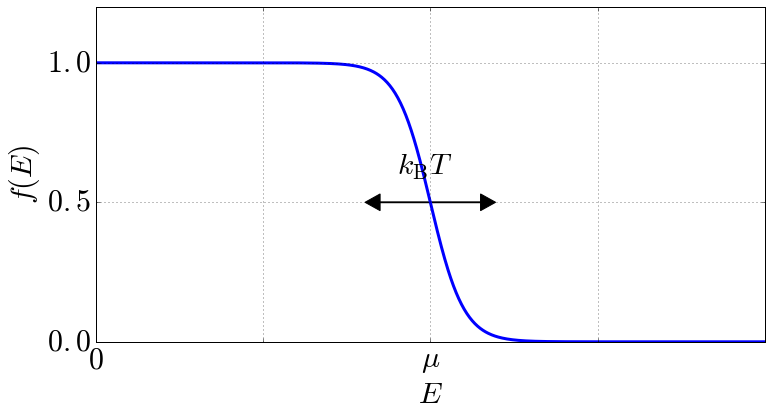
\includegraphics[width=0.2\textwidth]{Fig/fermi_eloszlas}
\par\end{centering}
\caption{Fermi-Dirac eloszl�s}
\end{wrapfigure}%


\subsection*{Z�rus h�m�rs�klet}

Hat�rozzuk meg egy h�rom dimenzi�s Fermi-g�z r�szecsk�inek �s energi�j�nak
�tlag�t ha a rendszer z�rus h�m�rs�kleten van. Tegy�k fel hogy a diszperzi�s
rel�ci� 
\begin{equation}
\varepsilon(\vec{k})=\frac{\left|\hbar\vec{k}\right|^{2}}{2m},
\end{equation}
alak� teh�t az �llapots�r�s�g 
\begin{equation}
\varrho\left(E\right)=(2s+1)V2\pi\left(\frac{2m}{h^{2}}\right)^{3/2}\sqrt{E}=\alpha V\sqrt{E}.
\end{equation}
A r�szecsk�k sz�m�nak v�rhat� �rt�ke z�rus h�m�rs�kleten teh�t 
\begin{eqnarray}
N & = & \int_{0}^{\infty}\frac{\varrho\left(E\right)}{\mathrm{e}^{\beta\left(E-\mu\right)}+1}\mathrm{d}E\underset{T\rightarrow0}{=}\int_{0}^{\mu}\varrho\left(E\right)\mathrm{d}E,\\
 & = & \alpha V\int_{0}^{\mu}\sqrt{E}\mathrm{d}E=\alpha V\frac{2}{3}\mu^{3/2},\nonumber 
\end{eqnarray}
azaz a k�miai potenci�l: 
\begin{equation}
\mu=\left(\frac{3}{2}\frac{N}{V}\frac{1}{\alpha}\right)^{2/3}.
\end{equation}
Hasonl� meggondol�sokb�l az energia v�rhat� �rt�ke
\begin{eqnarray}
\left\langle E\right\rangle  & = & \int_{0}^{\infty}\frac{E\varrho\left(E\right)}{\mathrm{e}^{\beta\left(E-\mu\right)}+1}\mathrm{d}E\underset{T\rightarrow0}{=}\int_{0}^{\mu}E\varrho\left(E\right)\mathrm{d}E\\
 & = & \alpha V\int_{0}^{\mu}E^{3/2}\mathrm{d}E=\alpha V\frac{2}{5}\mu^{5/2}.\nonumber 
\end{eqnarray}
Felhaszn�lva a fenti k�t �sszef�gg�st az energi�ra �s a k�miai potenci�lra
�s a (\ref{eq:qgaz-pv_nu_per_d}) �llapotegyenletet kapjuk hogy 
\begin{equation}
p=\frac{2}{3}\frac{\left\langle E\right\rangle }{V}=\frac{2}{3}\times\frac{2}{5}\alpha\left(\frac{3}{2}\frac{N}{V}\frac{1}{\alpha}\right)^{5/3}.
\end{equation}
\newpage{}

\subsection*{V�ges h�m�rs�klet k�t dimenzi�ban}

V�ges h�m�rs�kleten �ltal�ban nem tudjuk elv�gezni azokat az integr�lokat
melyekben a Fermi-f�ggv�ny szerepel. Ha viszont k�t dimenzi�s nem
relativisztikus rendszert vizsg�lunk akkor a r�szecsk�k sz�m�t z�rt
alakra tudjuk hozni!

Vegy�k �szre hogy k�t dimenzi�ban $d=2$ egy nem relativisztikus rendszer
�llapots�r�s�ge nem f�gg az energi�t�l!
\begin{equation}
\varrho_{2D}\left(E\right)=2D.
\end{equation}
Ekkor a r�szecsk�k sz�ma
\begin{eqnarray}
N & = & \int_{0}^{\infty}\frac{\varrho\left(E\right)}{\mathrm{e}^{\beta\left(E-\mu\right)}+1}\mathrm{d}E\\
 & = & 2D\int_{0}^{\infty}\frac{1}{\mathrm{e}^{\beta\left(E-\mu\right)}+1}\mathrm{d}E,\ x=\mathrm{e}^{\beta\left(E-\mu\right)},\ \mathrm{d}E=\frac{\mathrm{d}x}{\beta x}\nonumber \\
 & = & \frac{2D}{\beta}\int_{\mathrm{e}^{-\beta\mu}}^{\infty}\frac{1}{x}\frac{1}{x+1}\mathrm{d}x=\frac{2D}{\beta}\left[\int_{\mathrm{e}^{-\beta\mu}}^{\infty}\frac{1}{x}-\frac{1}{x+1}\mathrm{d}x\right]\nonumber \\
 & = & \frac{2D}{\beta}\left[\ln\frac{x}{x+1}\right]_{\mathrm{e}^{-\beta\mu}}^{\infty}=\frac{2D}{\beta}\ln\left(1+\mathrm{e}^{\beta\mu}\right)\nonumber 
\end{eqnarray}
kapjuk teh�t, hogy
\begin{equation}
\mathrm{e}^{\beta\mu}=\mathrm{e}^{\frac{\beta N}{2D}}-1,
\end{equation}
melyb�l a k�miai potenci�l kifejezhet� a h�m�rs�klet f�ggv�ny�ben
\begin{equation}
\mu=\frac{\ln\left(\mathrm{e}^{\frac{\beta N}{2D}}-1\right)}{\beta}.
\end{equation}
Az energia v�rhat��rt�k�t m�r nem tudjuk z�rt alakra hozni. A felmer�l�
integr�l
\begin{equation}
F_{j}(x)=\frac{1}{\Gamma\left(j+1\right)}\int_{0}^{\infty}\frac{t^{j}}{\mathrm{e}^{t-x}+1}\mathrm{d}t
\end{equation}
alak� melyet \href{https://en.wikipedia.org/wiki/Complete_Fermi\%E2\%80\%93Dirac_integral}{Fermi-Dirac integr�lnak}
h�vnak.

L�ttuk hogy a kvantumos eloszl�sf�ggv�nyeket �rtelmezhetj�k m�rtani
�sszegk�nt (\ref{eq:q_eloszlas_mertani}).
\begin{equation}
\frac{1}{\mathrm{e}^{\beta\left(E-\mu\right)}+1}=\mathrm{e}^{-\beta\left(E-\mu\right)}\sum_{l=0}\left(-1\right)^{l}\mathrm{e}^{-\beta l\left(E-\mu\right)}.
\end{equation}
Hat�rozzuk meg az fent vizsg�lt k�tdimenzi�s rendszer r�szecskesz�m�t
�s energia v�rhat� �rt�k�t magas h�m�rs�kleten, azaz amikor a m�rtani
sor helyett csak az els� k�t tagot vessz�k figyelembe!
\begin{equation}
N=2D\int_{0}^{\infty}\frac{1}{\mathrm{e}^{\beta\left(E-\mu\right)}+1}\mathrm{d}E\approx2D\int_{0}^{\infty}\mathrm{e}^{-\beta\left(E-\mu\right)}\left[1-\mathrm{e}^{-\beta\left(E-\mu\right)}+\dots\right]\mathrm{d}E=\frac{2D}{\beta}\mathrm{e}^{\beta\mu}\left[1-\frac{\mathrm{e}^{\beta\mu}}{2}+\dots\right]
\end{equation}
Ebb�l megtartva az els� k�t tagot ($l=0,1$)
\begin{equation}
\frac{N\beta}{2D}\left(1+\frac{\mathrm{e}^{\beta\mu}}{2}+\dots\right)=\mathrm{e}^{\beta\mu}
\end{equation}
Az energia hasonl�an
\begin{equation}
\left\langle E\right\rangle \approx2D\int_{0}^{\infty}E\mathrm{e}^{-\beta\left(E-\mu\right)}\left[1-\mathrm{e}^{-\beta\left(E-\mu\right)}+\dots\right]\mathrm{d}E=\frac{2D}{\beta^{2}}\mathrm{e}^{\beta\mu}\left[1-\frac{\mathrm{e}^{\beta\mu}}{4}+\dots\right]
\end{equation}
Vezet� rendben vissza �rva $\mathrm{e}^{\beta\mu}\approx\frac{N\beta}{2D}$-t:
\begin{equation}
\left\langle E\right\rangle \approx\frac{N}{\beta}\left[1-\frac{N\beta}{8D}+\dots\right]
\end{equation}
Vegy�k �szre hogy mivel $D\propto V$ (azaz extenz�v mennyis�g) a
z�r�jelben megjelen� tag intenz�v!

\subsection*{Kvantumkorrekci�k magas h�m�rs�kleten a h�rom dimenzi�s ultrarelativisztikus
Fermi-g�zban}

\begin{equation}
E(\vec{k})=c\left|\hbar\vec{k}\right|,\ d=3,\nu=1\label{eq:ultrarel-idgaz-disprel}
\end{equation}
\begin{equation}
\varrho(E)=g\frac{4\pi V}{\left(hc\right)^{3}}E^{2}=AE^{2}\label{eq:ultrarel-idgaz-allapotsuruseg}
\end{equation}
A r�szecsk�k $N$ sz�ma �s az energia $E$ v�rhat� �rt�ke az (\ref{eq:altalanos-id-qgaz-reszcskeszam})
�s (\ref{eq:atalanos-id-qgaz-energia}) alapj�n 
\begin{equation}
N=\int_{0}^{\infty}\frac{\varrho\left(E\right)}{\mathrm{e}^{\beta\left(E-\mu\right)}+1}\mathrm{d}E\approx A\Gamma\left(3\right)\frac{\mathrm{e}^{\beta\mu}}{\beta^{3}}\left(1-\frac{\mathrm{e}^{\beta\mu}}{2^{3}}+\dots\right)=g\frac{4\pi V}{\left(hc\right)^{3}}\frac{\mathrm{e}^{\beta\mu}2}{\beta^{3}}\left(1-\frac{\mathrm{e}^{\beta\mu}}{8}+\dots\right),\label{eq:ultrarel-id-qgaz-N}
\end{equation}
illetve 
\begin{equation}
\left\langle E\right\rangle =\int_{0}^{\infty}\frac{E\varrho\left(E\right)}{\mathrm{e}^{\beta\left(E-\mu\right)}+1}\mathrm{d}E\approx g\frac{4\pi V}{\left(hc\right)^{3}}\frac{\mathrm{e}^{\beta\mu}6}{\beta^{4}}\left(1-\frac{\mathrm{e}^{\beta\mu}}{2^{4}}+\dots\right).\label{eq:ultrarel-id-qgaz-E}
\end{equation}
Az egy r�szecsk�re jut� �tlagos energia
\begin{equation}
\frac{\left\langle E\right\rangle }{N}=\frac{\frac{3}{\beta}\left(1-\frac{\mathrm{e}^{\beta\mu}}{2^{4}}+\dots\right)}{\left(1-\frac{\mathrm{e}^{\beta\mu}}{8}+\dots\right)}\approx\frac{3}{\beta}\left(1+\frac{\mathrm{e}^{\beta\mu}}{2^{4}}\dots\right)\label{eq:ultrarel-id-qgaz-EpN}
\end{equation}
Vezet� rendben $\mathrm{e}{}^{\beta\mu}$-t kifejezve (\ref{eq:ultrarel-id-qgaz-N})-b�l
kapjuk hogy
\begin{equation}
\mathrm{e}^{\beta\mu}\approx\frac{N}{V}\frac{\left(\beta hc\right)^{3}}{g8\pi},\label{eq:ultrarel-id-qgaz-expbetamu}
\end{equation}
Vissza helyettes�tve (\ref{eq:ultrarel-id-qgaz-EpN})-be 
\begin{equation}
\frac{\left\langle E\right\rangle }{N}\approx\frac{3}{\beta}\left(1+\frac{N}{V}\frac{\left(\beta hc\right)^{3}}{128g\pi}\dots\right).\label{eq:ultrarel-id-qgaz-EpN-munelkul}
\end{equation}
�rdemes a klasszikus esetb�l kapott eredm�nnyel �sszehasonl�tani:
\begin{equation}
\left\langle E\right\rangle =3Nk_{\mathrm{B}}T.
\end{equation}
A (\ref{eq:qgaz-pv_nu_per_d}) kifejez�s szerint az ide�lis kvantumg�z
energi�ja kifejezhet� a nyom�s �s a t�rfogat szorzat�val 
\begin{equation}
pV=\frac{1}{3}\left\langle E\right\rangle .
\end{equation}
Kapjuk teh�t hogy az ultrarelativisztikus ide�lis g�z �llapotegyenlete
magas h�m�rs�kleten: 
\begin{equation}
pV=Nk_{\mathrm{B}}T\left(1+\frac{N}{V}\frac{\left(\beta hc\right)^{3}}{128g\pi}\dots\right)\label{ultrarel-idqgaz-allapotegyenlet}
\end{equation}
Hat�rozzuk most meg az entr�pia kvantumos korrekci�it magas h�m�rs�kleten!
C�lszer� a Gibbs-Duhem-rel�ci�t seg�ts�g�l h�vni
\begin{equation}
E=TS-pV+\mu N
\end{equation}
\begin{equation}
S=\frac{N}{T}\left(\frac{4}{3}\frac{E}{N}-\mu\right)\label{eq:ultrarel-id-q-gaz-Gibbs-Duuhem-S}
\end{equation}
Sz�ks�g�nk lesz teh�t a k�miai potenci�l magas h�m�rs�klet� k�zel�t�s�re
is! Induljunk ki (\ref{eq:ultrarel-id-qgaz-N})-b�l! Kihaszn�lva hogy
$\mathrm{e}^{\beta\mu}$ kicsi kapjuk hogy
\begin{equation}
\mathrm{e}^{\beta\mu}\approx N\frac{\left(hc\right)^{3}\beta^{3}}{g8\pi V}\left(1+\frac{\mathrm{e}^{\beta\mu}}{8}+\dots\right)
\end{equation}
a jobboldalon $\mathrm{e}^{\beta\mu}$-t a vezet�rendj�vel helyettes�tve
(\ref{eq:ultrarel-id-qgaz-expbetamu})
\begin{eqnarray}
\mathrm{e}^{\beta\mu} & \approx & N\frac{\left(hc\right)^{3}\beta^{3}}{g8\pi V}\left(1+\frac{N\left(hc\right)^{3}\beta^{3}}{g64\pi V}+\dots\right)\\
\mu & \approx & \frac{1}{\beta}\ln\left(\frac{N\left(hc\right)^{3}\beta^{3}}{g8\pi V}\right)+\frac{N\left(hc\right)^{3}\beta^{2}}{g64\pi V}
\end{eqnarray}
visszahelyettes�tve (\ref{eq:ultrarel-id-qgaz-EpN})-t �s a fenti
kifejez�st (\ref{eq:ultrarel-id-q-gaz-Gibbs-Duuhem-S})-be kapjuk
hogy 
\begin{eqnarray}
S & = & \frac{N}{T}\left(\frac{4}{\beta}\left(1+\frac{N}{V}\frac{\left(\beta hc\right)^{3}}{128g\pi}\right)-\frac{1}{\beta}\ln\left(\frac{N\left(hc\right)^{3}\beta^{3}}{g8\pi V}\right)-\frac{N\left(hc\right)^{3}\beta^{2}}{g64\pi V}\right)\nonumber \\
S & = & \frac{N}{T}\left(\frac{4}{\beta}-\frac{1}{\beta}\ln\left(\frac{N\left(hc\right)^{3}\beta^{3}}{g8\pi V}\right)+\left(4\frac{N}{V}\frac{\left(hc\right)^{3}\beta^{2}}{128g\pi}\right)-\frac{N\left(hc\right)^{3}\beta^{2}}{g64\pi V}\right)\nonumber \\
S & = & \frac{N}{T}\left(\frac{4}{\beta}-\frac{1}{\beta}\ln\left(\frac{N\left(hc\right)^{3}\beta^{3}}{g8\pi V}\right)+\left(\frac{N}{V}\frac{\left(hc\right)^{3}\beta^{2}}{64g\pi}\right)\right)\nonumber \\
S & = & Nk_{\mathrm{B}}\left(4-\ln\left(\frac{1}{8\pi}\frac{N}{gV}\left(\frac{hc}{k_{\mathrm{B}}T}\right)^{3}\right)+\frac{1}{64\pi}\frac{N}{gV}\left(\frac{hc}{k_{\mathrm{B}}T}\right)^{3}\right)
\end{eqnarray}
A fenti kifejez�s els� k�t tagja megegyezik a klasszikus ultrarelativisztikus
ide�lis g�z entr�pi�j�val. 

Hat�rozzunk meg v�g�l k�t m�rhet� mennyis�g, az �lland� t�rfogaton
$C_{V}$ m�rt fajh� illetve a $\kappa_{T}$ izoterm kompresszibilit�s
magash�m�rs�klet� viselked�s�t is! Kezdj�k $C_{V}$-vel! Kiindulva
(\ref{eq:ultrarel-id-qgaz-EpN-munelkul})-b�l kapjuk hogy 
\begin{eqnarray}
C_{V} & = & \left.\partial_{T}E\right|_{V}=\\
 & =\partial_{T} & 3N\left(k_{\mathrm{B}}T\right)\left(1+\frac{N}{V}\frac{\left(hc\right)^{3}}{128g\pi\left(k_{\mathrm{B}}T\right)^{3}}\dots\right)\nonumber \\
 & = & 3k_{\mathrm{B}}N\left(1-\frac{N}{V}\frac{1}{64g\pi}\left(\frac{hc}{k_{\mathrm{B}}T}\right)^{3}\right)\nonumber 
\end{eqnarray}
A kompresszibilit�s 
\begin{equation}
\kappa_{T}=-\frac{1}{V}\left.\partial_{p}V\right|_{T,N}
\end{equation}
meghat�roz�s�hoz induljunk ki az (\ref{ultrarel-idqgaz-allapotegyenlet})
�llapot egyenletb�l.
\begin{eqnarray}
V & = & \frac{Nk_{\mathrm{B}}T}{p}\left(1+\frac{N}{V}\frac{\left(\beta hc\right)^{3}}{128g\pi}\dots\right)\\
 & \approx & \frac{Nk_{\mathrm{B}}T}{p}\left(1+\frac{p}{k_{\mathrm{B}}T}\frac{\left(\beta hc\right)^{3}}{128g\pi}\dots\right)\\
 & = & \frac{Nk_{\mathrm{B}}T}{p}+N\frac{\left(\beta hc\right)^{3}}{128g\pi}
\end{eqnarray}
ahol $\frac{N}{V}$-t ism�t az els� rendbeli �rt�k�vel k�zel�tett�k
a m�sodik tagban.
\begin{eqnarray}
-\frac{1}{V}\partial_{p}V & = & -\frac{1}{V}\left(-\frac{Nk_{\mathrm{B}}T}{p^{2}}\right)\\
 & = & \frac{p}{Nk_{\mathrm{B}}T}\left(1-\frac{p}{k_{\mathrm{B}}T}\frac{\left(\beta hc\right)^{3}}{128g\pi}\dots\right)\frac{Nk_{\mathrm{B}}T}{p^{2}}\\
\kappa_{T} & = & \frac{1}{p}\left(1-\frac{p}{k_{\mathrm{B}}T}\frac{\left(\beta hc\right)^{3}}{128g\pi}\dots\right)
\end{eqnarray}

\begin{xca}
Hat�rozzuk meg az �lland� nyom�son vett fajh� magash�m�rs�klet� kvantum
korrekci�it ultrarelativisztikus Fermi-g�z eset�ben.
\end{xca}
$\ $
\begin{xca}
Hat�rozzuk meg az ultrarelativsztikus Bose-g�z magas h�m�rs�klet�
korrekci�it! Vizsg�ljuk meg a Fermi-g�z t�rgyal�s�n�l kisz�molt mennyis�geket! 
\end{xca}

\subsection*{Alacsony h�m�rs�klet� ultrarelativisztikus Fermi-g�z}

\begin{shaded}%
\textbf{Sommerfeld sorfejt�s:}
\begin{equation}
\int_{0}^{\infty}\varphi(E)f(E)\mathrm{d}E\approx\int_{0}^{\mu}\varphi(E)\mathrm{d}E+\frac{\pi^{2}}{6}\left(k_{\mathrm{B}}T\right)^{2}\varphi'(\mu)+\dots
\end{equation}
\end{shaded}
\begin{equation}
\varrho(E)=g\frac{4\pi V}{\left(hc\right)^{3}}E^{2}=AE^{2}
\end{equation}
Hat�rozzuk meg el�sz�r az energia �s a r�szecskesz�m �rt�k�t z�rus
h�m�rs�kleten!
\begin{equation}
N=\int_{0}^{\mu}\varrho\left(E\right)\mathrm{d}E=g\frac{4\pi V}{3\left(hc\right)^{3}}\mu^{3}
\end{equation}
A k�miai potenci�l teh�t z�rus h�m�rs�kleten
\begin{equation}
\mu_{0}=\left(\frac{N3}{g4\pi V}\right)^{1/3}\left(hc\right).
\end{equation}
Az energia 
\begin{eqnarray}
\left\langle E\right\rangle  & = & \int_{0}^{\mu}E\varrho\left(E\right)\mathrm{d}E=g\frac{\pi V}{\left(hc\right)^{3}}\mu^{4}\\
 & = & g\pi Vhc\left(\frac{N3}{g4\pi V}\right)^{4/3}\nonumber 
\end{eqnarray}
Hat�rozzuk most meg az alacsony h�m�rs�klet� viselked�st!
\begin{eqnarray}
N & = & \int_{0}^{\infty}\varrho\left(E\right)f(E)\mathrm{d}E=\int_{0}^{\mu}\varrho\left(E\right)\mathrm{d}E+\frac{\pi^{2}}{6}\left(k_{\mathrm{B}}T\right)^{2}\varrho'\left(\mu\right)+\dots\\
 & = & g\frac{4\pi V}{3\left(hc\right)^{3}}\mu^{3}+\frac{\pi^{2}}{6}\left(k_{\mathrm{B}}T\right)^{2}g\frac{8\pi V}{\left(hc\right)^{3}}\mu\nonumber \\
 & = & g\frac{4\pi V}{\left(hc\right)^{3}}\left(\frac{\mu^{3}}{3}+\frac{\pi^{2}}{3}\left(k_{\mathrm{B}}T\right)^{2}\mu\right)\nonumber 
\end{eqnarray}
ebb�l 
\begin{eqnarray}
\frac{N\left(hc\right)^{3}3}{g4\pi V} & = & \mu^{3}+\pi^{2}\left(k_{\mathrm{B}}T\right)^{2}\mu\\
\mu_{0}^{3} & = & \mu^{3}+\pi^{2}\left(k_{\mathrm{B}}T\right)^{2}\mu\\
 & \approx & \mu^{3}\left(1+\pi^{2}\left(\frac{k_{\mathrm{B}}T}{\mu_{0}}\right)^{2}\right)
\end{eqnarray}
A k�miai potenci�l els� v�ges h�m�rs�klet� korrekci�ja teh�t 
\begin{equation}
\mu\approx\mu_{0}\left(1-\frac{\pi^{2}}{3}\left(\frac{k_{\mathrm{B}}T}{\mu_{0}}\right)^{2}\right).\label{eq:ultrarel-id-qgaz-BS-kempot}
\end{equation}
Az energia v�rhat� �rt�ke
\begin{eqnarray}
\left\langle E\right\rangle  & = & \int_{0}^{\infty}E\varrho\left(E\right)f(E)\mathrm{d}E=\int_{0}^{\mu}E\varrho\left(E\right)\mathrm{d}E+\frac{\pi^{2}}{6}\left(k_{\mathrm{B}}T\right)^{2}\left(E\varrho\right)'\left(\mu\right)\\
 & = & g\frac{4\pi V}{\left(hc\right)^{3}}\left(\frac{\mu^{4}}{4}+\frac{\pi^{2}}{6}\left(k_{\mathrm{B}}T\right)^{2}3\mu^{2}+\dots\right)
\end{eqnarray}
Egy r�szecsk�re jut� energia
\begin{eqnarray}
\frac{\left\langle E\right\rangle }{N} & = & \frac{\left(\frac{\mu^{4}}{4}+\frac{\pi^{2}}{6}\left(k_{\mathrm{B}}T\right)^{2}3\mu^{2}+\dots\right)}{\left(\frac{\mu^{3}}{3}+\frac{\pi^{2}}{6}\left(k_{\mathrm{B}}T\right)^{2}2\mu+\dots\right)}\\
 & = & \frac{\frac{\mu^{4}}{4}\left(1+2\pi^{2}\left(\frac{k_{\mathrm{B}}T}{\mu}\right)^{2}+\dots\right)}{\frac{\mu^{3}}{3}\left(1+\pi^{2}\left(\frac{k_{\mathrm{B}}T}{\mu}\right)^{2}+\dots\right)}\nonumber \\
 & \approx & \frac{3}{4}\mu\left(1+\pi^{2}\left(\frac{k_{\mathrm{B}}T}{\mu_{0}}\right)^{2}+\dots\right)\nonumber \\
 & \approx & \frac{3}{4}\mu_{0}\left(1-\frac{\pi^{2}}{3}\left(\frac{k_{\mathrm{B}}T}{\mu_{0}}\right)^{2}\right)\left(1+\pi^{2}\left(\frac{k_{\mathrm{B}}T}{\mu_{0}}\right)^{2}+\dots\right)\nonumber \\
\frac{\left\langle E\right\rangle }{N} & \approx & \frac{3}{4}\mu_{0}\left(1+\frac{2}{3}\pi^{2}\left(\frac{k_{\mathrm{B}}T}{\mu_{0}}\right)^{2}\right)
\end{eqnarray}
Ennek ismeret�ben �s felhaszn�lva az (\ref{eq:qgaz-pv_nu_per_d})
�sszef�gg�st, az �llapot egyenletre vonatkoz� alacsony h�m�rs�klet�
korrekci�k meghat�rozhat�ak:
\begin{equation}
pV=\frac{1}{3}\left\langle E\right\rangle =\frac{1}{4}\mu_{0}N\left(1+\frac{2}{3}\pi^{2}\left(\frac{k_{\mathrm{B}}T}{\mu_{0}}\right)^{2}\right)
\end{equation}
A fajh� pedig 
\begin{equation}
C_{V}=\partial_{T}\left\langle E\right\rangle =\pi^{2}k_{\mathrm{B}}N\left(\frac{k_{\mathrm{B}}T}{\mu_{0}}\right).
\end{equation}


\subsection*{Milyen h�m�rs�kleten t�nik el a k�miai potenci�l?}

Hat�rozzuk meg azt a kritikus h�m�rs�kletet ahol egy ide�lis nem reativisztikus
Fermi-g�z k�miai potenci�lja elt�nik!
\begin{equation}
\varrho(E)=\alpha V\sqrt{E}.
\end{equation}
Keress�k teh�t azt a $T_{1}$ h�m�rs�kletet ahol 
\begin{equation}
N=\int_{0}^{\infty}\frac{\varrho\left(E\right)}{\mathrm{e}^{\beta_{1}E}+1}\mathrm{d}E=\int_{0}^{\infty}\frac{\alpha V\sqrt{E}}{\mathrm{e}^{\beta_{1}E}+1}\mathrm{d}E.
\end{equation}
Legyen 
\begin{eqnarray}
\beta_{1}E & = & x^{2},\ \sqrt{E\beta_{1}}=x,\\
\beta_{1}\mathrm{d}E & = & 2x\mathrm{d}x,
\end{eqnarray}
ekkor
\begin{eqnarray}
N & = & \frac{\alpha V}{\sqrt{\beta_{1}}}\int_{0}^{\infty}\frac{x}{\mathrm{e}^{x^{2}}+1}\frac{2x\mathrm{d}x}{\beta_{1}},\\
 & = & 2\alpha V\left(k_{\mathrm{B}}T_{1}\right)^{3/2}\int_{0}^{\infty}\frac{x^{2}}{\mathrm{e}^{x^{2}}+1}\mathrm{d}x.\label{eq:fermion-zerus-mu-N}
\end{eqnarray}
Term�szetesen z�rus h�m�rs�kleten a k�miai potenci�l v�ges �s ekkor
\begin{equation}
N=\int_{0}^{\mu}\alpha V\sqrt{E}\mathrm{d}E=\frac{\alpha2V}{3}\mu^{3/2}=\frac{\alpha2V}{3}\left(k_{\mathrm{B}}T_{F}\right)^{3/2}.\label{eq:fermion-zerus-T-N}
\end{equation}
A (\ref{eq:fermion-zerus-mu-N}) �s (\ref{eq:fermion-zerus-T-N})
kifejez�sek h�nyados�b�l kapjuk teh�t hogy
\begin{eqnarray}
1 & = & \frac{2\alpha V\left(k_{\mathrm{B}}T_{1}\right)^{3/2}}{\frac{\alpha2V}{3}\left(k_{\mathrm{B}}T_{F}\right)^{3/2}}\int_{0}^{\infty}\frac{x^{2}}{\mathrm{e}^{x^{2}}+1}\mathrm{d}x,\\
1 & = & \frac{1}{3}\left(\frac{T_{1}}{T_{F}}\right)\underbrace{\int_{0}^{\infty}\frac{x^{2}}{\mathrm{e}^{x^{2}}+1}\mathrm{d}x}_{\approx0.339}\rightarrow\left(\frac{T_{F}}{T_{1}}\right)\approx1.01139.
\end{eqnarray}


\section{Ide�lis Bose-g�z}

\subsection*{Foton g�z r�szecskesz�ma}

\begin{wrapfigure}{o}{0.3\columnwidth}%
\begin{centering}
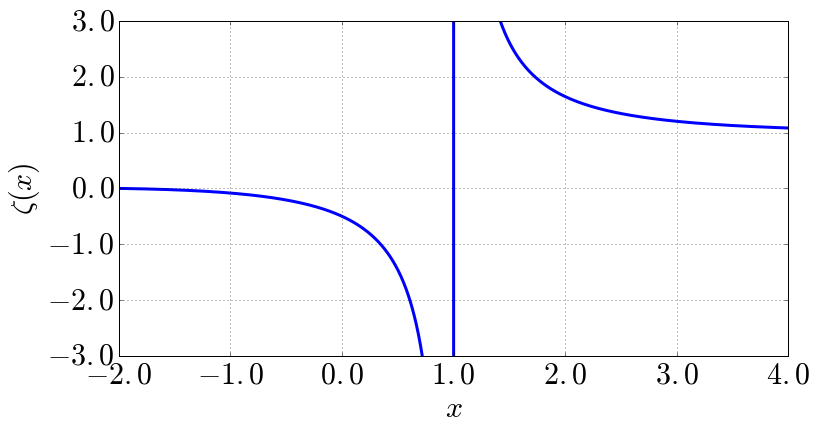
\includegraphics[width=0.3\textwidth]{Fig/zeta}
\par\end{centering}
\caption{Riemann-f�le $\zeta-$f�ggv�ny}
\end{wrapfigure}%

Hat�rozzuk meg egy $T$ h�m�rs�klet� �regben l�v� fotonok $N$ sz�m�t!
A foton g�zra tekinthet�nk �gy mint egy utrarelativisztikus kvantum
g�zra melyet $\mu=0$ k�miai potenci�llal rendelkez� Bose-Einstein-statisztik�t
k�vet� r�szecsk�k alkotnak, melynek a polariz�ci�b�l sz�rmaz� degener�ci�foka
$g=2$ ! A diszperzi�s rel�ci� teh�t ism�t (\ref{eq:ultrarel-idgaz-disprel})
m�g az �llapots�r�s�get �jfent (\ref{eq:ultrarel-idgaz-allapotsuruseg})
adja: 
\begin{equation}
E(\vec{k})=c\left|h\vec{k}\right|,
\end{equation}
\begin{equation}
\varrho(E)=g\frac{4\pi V}{\left(hc\right)^{3}}E^{2}=AE^{2}.
\end{equation}
Az �ltal�nos ide�lis Bose-g�z r�szecskesz�m v�rhat��rt�ke (\ref{eq:altalanos-id-qgaz-reszcskeszam})
szerint 
\begin{equation}
\left\langle N\right\rangle =A\Gamma\left(\frac{d}{\nu}\right)\frac{\mathrm{e}^{\beta\mu}}{\beta^{\frac{d}{\nu}}}\sum_{l=0}\frac{\mathrm{e}^{\beta\mu l}}{\left(l+1\right)^{\frac{d}{\nu}}}\label{eq:altalanos-bose-gaz-reszecskeszam}
\end{equation}
A mi eset�nkben $d=3,\ \nu=1$ �s $\mu=0$ teh�t a r�szecskesz�m v�rhat��rt�k
az 
\begin{equation}
\left\langle N\right\rangle =A\frac{\Gamma\left(3\right)}{\beta^{3}}\sum_{l=1}^{\infty}\frac{1}{l^{3}}
\end{equation}
alakot �lti. Az �sszegben felismerhetj�k a Riemann-f�le $\zeta(z)$-f�ggv�nyt.

\begin{wraptable}{r}{0.2\columnwidth}%
\begin{centering}
\begin{tabular}{|c|c|}
\hline 
$z$ & $\zeta(z)$\tabularnewline
\hline 
\hline 
$-1$ & $-\frac{1}{12}$\tabularnewline
\hline 
$0$ & $-\frac{1}{2}$\tabularnewline
\hline 
$1$ & $\infty$\tabularnewline
\hline 
$2$ & $\frac{\pi^{2}}{6}$\tabularnewline
\hline 
$3$ & $1.202$\tabularnewline
\hline 
$4$ & $\frac{\pi^{4}}{90}$\tabularnewline
\hline 
$3/2$ & $2.612$\tabularnewline
\hline 
$5/2$ & $1.314$\tabularnewline
\hline 
\end{tabular}
\par\end{centering}
\caption{Riemann-f�le $\zeta$-f�ggv�ny n�h�ny �rt�ke}
\end{wraptable}%
\parbox[t]{0.7\columnwidth}{%
\begin{shaded}%
\textbf{\href{https://hu.wikipedia.org/wiki/Riemann-f\%C3\%A9le_z\%C3\%A9ta-f\%C3\%BCggv\%C3\%A9ny}{Riemann-Zeta-f�ggv�ny}}
\begin{eqnarray}
\zeta\left(z\right) & = & \sum_{n=1}^{\infty}\frac{1}{n^{z}}\\
 & = & \frac{1}{\Gamma\left(z\right)}\int_{0}^{\infty}\frac{x^{z-1}}{\mathrm{e}^{x}-1}\mathrm{d}x
\end{eqnarray}
\end{shaded}%
}

A $\zeta$-f�ggv�ny seg�ts�g�vel a r�szecskesz�m v�rhat� �rt�ke teh�t:

\begin{eqnarray}
\left\langle N\right\rangle  & = & 2\frac{4\pi V}{\left(hc\right)^{3}}\frac{\Gamma\left(3\right)\zeta\left(3\right)}{\beta^{3}}=\frac{16\pi V}{\left(hc\beta\right)^{3}}\zeta\left(3\right)\\
 & = & V\frac{2\zeta\left(3\right)}{\pi^{2}}\left(\frac{k_{\mathrm{B}}T}{\hbar c}\right)^{3}
\end{eqnarray}

\newpage{}

\subsection*{A k�miai potenci�l viselked�se a kritikus h�m�rs�klet k�zel�ben}

Tudjuk hogy a kondenz�ci�s h�m�rs�klet alatt a $\mu$ k�miai potenci�l
�rt�ke z�rus. Vizsg�ljuk meg hogy mik�nt viselkedik a k�miai potenci�l
a kritikus h�m�rs�klet felett de ahhoz k�zeli h�m�rs�kleten! A vizsg�l�d�s
sor�n sz�ks�g�nk lesz a Bose-Einstein integr�lok n�h�ny tulajdons�g�ra.
Foglaljuk az al�bbiakban �ssze ezeket. 

\begin{shaded}%
\textbf{Bose-Einstein- �s Fermi-Dirac-integr�lok:}
\begin{equation}
F^{\pm}\left(s,\alpha\right)=\frac{1}{\Gamma\left(s\right)}\int_{0}^{\infty}\frac{x^{s-1}\mathrm{d}x}{\mathrm{e}^{x+\alpha}\pm1}\begin{cases}
+: & \mbox{Fermi-Dirac}\\
-: & \mbox{Bose-Einstein},\ \mbox{Re}(s)>1,\alpha>0
\end{cases}
\end{equation}
Deriv�ltak $\alpha$-szerint:
\begin{equation}
\frac{\partial^{n}F^{\pm}\left(s,\alpha\right)}{\partial\alpha^{n}}=\left(-1\right)^{n}F^{\pm}\left(s-n,\alpha\right)
\end{equation}
\href{http://journals.aps.org/pr/pdf/10.1103/PhysRev.83.678}{Bose-Einstein-integr�lok k�zel�t�se}:
\begin{equation}
F^{-}\left(s,\alpha\right)\approx\zeta\left(s\right)+\Gamma\left(1-s\right)\alpha^{s-1}\dots,\mbox{ha \ensuremath{s} nem pozit�v eg�sz �s \ensuremath{\alpha\ll}}1
\end{equation}
\end{shaded}

Vizsg�ljuk meg most a h�rom dimenzi�s nem relativisztikus Bose-g�z
k�miai potenci�lj�nak viselked�s�t a kritikus h�m�rs�klet k�zel�ben.
A Bose-g�z r�szecskesz�ma �ltal�nos esetben az al�bbiak szerint fejezhet�
ki a fenn defini�lt Bose-Einstein integr�lokkal
\begin{eqnarray}
N & = & \int_{0}^{\infty}\frac{\varrho\left(E\right)\mathrm{d}E}{\mathrm{e}^{\beta\left(E-\mu\right)}-1}=A\int_{0}^{\infty}\frac{E^{\frac{d}{\nu}-1}\mathrm{d}E}{\mathrm{e}^{\beta\left(E-\mu\right)}-1},\ E=\frac{x}{\beta},\ \frac{\mathrm{d}E}{\mathrm{d}x}=\frac{1}{\beta},\ \alpha=-\beta\mu\\
 & = & A\int_{0}^{\infty}\frac{\left(\frac{x}{\beta}\right)^{\frac{d}{\nu}-1}\frac{\mathrm{d}x}{\beta}}{\mathrm{e}^{x+\alpha}-1}=\frac{A}{\beta^{d/\nu}}\int_{0}^{\infty}\frac{x^{\frac{d}{\nu}-1}\mathrm{d}x}{\mathrm{e}^{x+\alpha}-1}\nonumber \\
 & = & \frac{A}{\beta^{d/\nu}}\Gamma\left(\frac{d}{\nu}\right)F^{-}\left(\frac{d}{\nu},\alpha\right)\nonumber 
\end{eqnarray}
Eset�nkben $d=3,\nu=2$. Vegy�k a r�szecskesz�m kifejez�sek h�nyados�t
$T_{c}$-n �s kicsivel $T_{c}$ felett! Bevezetve a $\beta_{c}=\frac{1}{k_{\mathrm{B}}T_{c}}$
jel�l�st 
\begin{eqnarray}
1 & = & \frac{\frac{A}{\beta^{\frac{3}{2}}}\Gamma\left(\frac{3}{2}\right)F^{-}\left(\frac{3}{2},\alpha\right)}{\frac{A}{\beta_{c}^{\frac{3}{2}}}\Gamma\left(\frac{3}{2}\right)F^{-}\left(\frac{3}{2},0\right)}\\
\left(\frac{T_{c}}{T}\right)^{\frac{3}{2}} & = & \frac{F^{-}\left(\frac{3}{2},\alpha\right)}{F^{-}\left(\frac{3}{2},0\right)}\approx\frac{\zeta\left(\frac{3}{2}\right)+\Gamma\left(-\frac{1}{2}\right)\alpha_{c}^{\frac{1}{2}}}{\zeta\left(\frac{3}{2}\right)}\\
\left(\frac{T_{c}}{T}\right) & = & \left(1-\frac{2\sqrt{\pi}}{\zeta\left(\frac{3}{2}\right)}\alpha_{c}^{\frac{1}{2}}\right)^{\frac{2}{3}}\approx1-\frac{4}{3}\frac{\sqrt{\pi}}{\zeta\left(\frac{3}{2}\right)}\alpha_{c}^{\frac{1}{2}}
\end{eqnarray}
Ahol kihaszn�ltuk hogy $\Gamma(-1/2)=-2\sqrt{\pi}$ �s bevezett�k
$\alpha_{c}=-\beta_{c}\mu$-t. Kifejezve a fenti kifejez�sb�l $\mu$-t
kapjuk hogy 
\begin{equation}
\mu=-k_{\mathrm{B}}T_{c}\left[\frac{3\zeta\left(\frac{3}{2}\right)}{4\sqrt{\pi}}\left(1-\frac{T_{c}}{T}\right)\right]^{2}\approx-k_{\mathrm{B}}T_{c}\left[\frac{3\zeta\left(\frac{3}{2}\right)}{4\sqrt{\pi}}\right]^{2}\left(\frac{T}{T_{c}}-1\right)^{2}
\end{equation}
ahol felhaszn�ltuk az $1-1/x\approx x-1$ k�zel�t�st mely $x\approx1$
eset�n igaz. Kapjuk teh�t hogy a k�miai potenci�l $T_{c}$ felett
kvadratikusan cs�kken!

\subsection*{Alacsony dimenzi�s Bose-g�z nem kondenz�l}

A h�rom dimenzi�s nem relativisztikus Bose-g�z eset�n a r�szecskesz�m
z�rus k�miai potenci�l eset�n egy v�ges �rt�khez tart. Az ebb�l ad�d�
koncepcion�lis paradoxon magyar�zata hogy egy kritikus h�m�rs�klet
alatt a r�szecsk�k jelent�s h�nyada a z�rus impulzus� �llapotba kondenz�l. 

Vizsg�ljuk meg az $N(\mu)$ kifejez�s viselked�s�t �ltal�nosabb esetben!
Kor�bban (\ref{eq:altalanos-bose-gaz-reszecskeszam}) l�ttuk hogy
�ltal�nos Bose-g�z eset�n a r�szecskesz�m 

\begin{equation}
N=A\Gamma\left(\frac{d}{\nu}\right)\frac{\mathrm{e}^{\beta\mu}}{\beta^{\frac{d}{\nu}}}\sum_{l=0}\frac{\mathrm{e}^{\beta\mu l}}{\left(l+1\right)^{\frac{d}{\nu}}}
\end{equation}
alakot �lti. A kondenz�ci�hoz sz�ks�ges �ltal�nos felt�tel teh�t hogy
az �sszeg v�ges legyen z�rus k�miai potenci�l eset�re! Ez a felt�tel
nyilv�n val�an teljes�l ha $\frac{d}{\nu}>1$! Egy illetve k�t dimenzi�s
nem relativisztikus g�z eset�n $\frac{d}{\nu}=1$ illetve $\frac{d}{\nu}=\frac{1}{2}$!
Azaz ezekben az esetekben az �sszeg $\mu=0$ -ra minden hat�ron t�l
n�! Azaz alacsony dimenzi�s nem relativisztikus rendszerekben nincs
Bose-kondenz�ci�. 

\part{K�lcs�nhat� rendszerek}

\section{Egy dimenzi�s Ising-model}

Vizsg�ljunk k�t �llapot� klasszikus spinek $S_{i}=\pm1$ egy dimenzi�s
rendszer�t. Legyen a rendszer v�ges �s rendelkezzen szabad peremfelt�tellel. 

\begin{equation}
H=-J\sum_{\left\langle ij\right\rangle }S_{i}S_{j}
\end{equation}
A kanonikus �llapot�sszeg 
\begin{equation}
Z=\sum_{\left\{ S_{i}\right\} }\mathrm{e^{\kappa S_{1}S_{2}}\dots e^{\kappa S_{N-1}S_{N}}},\ \kappa=\beta J
\end{equation}
Vegy�k �szre hogy ha az egyik v�gen l�v� spin-re elv�gezz�k az �sszeget
akkor az a mellette l�v� spin �rt�k�t�l f�ggetlen�l ugyan azt a j�rul�kot
fogja adni! 
\begin{equation}
\sum_{S_{N}=\pm1}e^{\kappa S_{N-1}S_{N}}=2\cosh\kappa.
\end{equation}
Kapjuk teh�t hogy 
\begin{equation}
Z_{N}=2\cosh\kappa Z_{N-1}.
\end{equation}
Figyelembe v�ve hogy 
\begin{equation}
Z_{1}=2,
\end{equation}
a teljes rendszer �llapot�sszege 
\begin{equation}
Z_{N}=2\left(2\cosh\kappa\right)^{N-1}.
\end{equation}
Hat�rozzuk meg a rendszer korrel�ci�s f�ggv�ny�t! Azaz az $\left\langle S_{i}S_{j}\right\rangle $
v�rhat��rt�ket! Ehhez el�sz�r tegy�k fel hogy a $\kappa$ csatol�s
nem homog�n hanem minden p�rra k�l�n k�l�n �rt�keket vehet fel! Ekkor
\begin{equation}
Z=2^{N}\prod_{p=1}^{N}\cosh\kappa_{p}.\label{eq:ising-chain-Z}
\end{equation}
Az �llapot�sszeg defin�ci�j�b�l nyilv�nval� hogy 
\begin{equation}
\frac{1}{Z}\frac{\partial^{n}Z}{\partial\kappa_{i}\partial\kappa_{i+1}\dots\partial\kappa_{i+n-1}}=\left\langle S_{i}\overbrace{S_{i+1}S_{i+1}}^{1}\underbrace{S_{i+2}S_{i+2}}_{1}S_{i+3}\dots S_{i+n-1}S_{i+n}\right\rangle =\left\langle S_{i}S_{i+n}\right\rangle 
\end{equation}
Vegy�k �szre hogy tetsz�leges k�t spin korrel�ci�s f�ggv�nye teh�t
kifejezhet� a fenti deriv�lt seg�ts�g�vel! A deriv�ltat viszont k�zvetlen�l
is elv�gezhetj�k az �llapot�sszeg (\ref{eq:ising-chain-Z}) kifejez�s�n!
\begin{equation}
\frac{1}{\left(2^{N}\prod_{p=1}^{N}\cosh\kappa_{i}\right)}\frac{\partial^{n}}{\partial\kappa_{i}\partial\kappa_{i+1}\dots\partial\kappa_{i+n-1}}\left(2^{N}\prod_{p=1}^{N}\cosh\kappa_{i}\right)=\prod_{p=i}^{i+n-1}\frac{\sinh\kappa_{i}}{\cosh\kappa_{i}}=\prod_{p=i}^{i+n-1}\tanh\kappa_{i}.
\end{equation}
Vissza�ll�tva a rendszer homogenit�s�t, azaz $\kappa_{i}=\kappa$
eset�n, 
\begin{equation}
\left\langle S_{i}S_{i+n}\right\rangle =\tanh^{n}\kappa=\mathrm{e}^{n\ln\tanh\kappa}.
\end{equation}
Mivel $\tanh\kappa<1$ez�rt a logaritmus el�jele mindig negat�v!
\begin{equation}
\left\langle S_{i}S_{i+n}\right\rangle =\mathrm{e}^{-an\frac{\left|\ln\tanh\kappa\right|}{a}}=\mathrm{e}^{-\frac{an}{\xi}}
\end{equation}
Ahol bevezett�k a korrel�ci�s hosszt mint 
\begin{equation}
\xi=\frac{a}{\left|\ln\tanh\kappa\right|},
\end{equation}
illetve $a$ egy a rendszerre jellemz� hossz mennyis�g (pl. a spinek
k�z�tti t�vols�g a val�s t�rben). Ha az alacsony h�m�rs�klet� viselked�st
vizsg�ljuk akkor $\beta\rightarrow\infty,\ \kappa\rightarrow\infty,\ \tanh\kappa\rightarrow1,\ \ln\tanh\kappa\rightarrow0$
teh�t $\xi\rightarrow\infty$. 

\end{document}
